\documentclass[openany]{r1090}                % web version
% \documentclass[print, openright]{r1090}      % print version (with margins)


\date{}

\newcommand\1{\texttt{1}}
\newcommand\0{\texttt{0}}



\begin{document}


\title[A Guide to Decoding Mode S and ADS-B Signals]{The 1090 Megahertz Riddle}
\author{Junzi}{Sun}


\begin{titlepage}

\thispagestyle{empty}

\vspace*{2\bigskipamount}

%% Print the title.
{\makeatletter
\titlestyle\bfseries\Huge\@title
\makeatother}

%% Print the optional subtitle.
{\makeatletter
\ifx\@subtitle\undefined\else
    \bigskip
    \titlefont\titleshape\LARGE\@subtitle
\fi
\makeatother}


\vspace*{8\bigskipamount}


%% Print the full name of the author.
\makeatletter
{\huge\titlefont\bfseries{Junzi}\ {SUN}}
\makeatother

\vspace*{8\bigskipamount}

\makeatletter
{\large\titlefont{TU Delft OPEN Publishing}}
\makeatother


\clearpage


\thispagestyle{empty}

\vspace*{25\bigskipamount}



Keywords: Aircraft Surveillance, Radar, Decoding, Mode~A/C, Mode~S, ADS-B, Comm-B, ELS, EHS, MRAR.

\medskip

Publisher: TU Delft OPEN Publishing

\vspace{4\bigskipamount}


Copyright \textcopyright\ 2020 by Junzi Sun

\medskip

Published under CC BY-NC-SA 4.0 license.

\medskip
ISBN: 978-94-6366-402-8

\medskip
\medskip
An electronic version of this dissertation is available at \\
\url{https://doi.org/10.34641/mg.11}

\end{titlepage}

% \maketitle

\dedication{
  This book is dedicated to my sons: William and Vincent
}

\setcounter{tocdepth}{1}
\tableofcontents

\chapter*{Preface}
% WHY THIS BOOK? WHY USEFUL? WHAT PURPOSE? 2/3 SENTENCES
% say this is second edition???

This book provides a practical guide to decoding ADS-B and other types of common Mode~S messages. It consolidates the information from various ICAO documentation and other literature to provide readers easy access to key knowledge of Mode~S and ADS-B and related topics. In this book, examples and sample Python code are used extensively to explain the decoding process.

Back in 2015, I joined Delft University of Technology to undertake PhD research on analyzing and modeling aircraft performance using open aircraft surveillance data. ADS-B data served as my primary data source.

Frustrated with the lack of open literature on ADS-B and Mode~S, I created a live online project to document my experience in decoding ADS-B data, the \emph{ADS-B Decoding Guide}. As the guide grew in popularity, I started to receive questions, feedback, suggestions from the research community all over the world. These inputs greatly helped me to fix and improve the content of the decoding guide.

At the same time, I also started to incorporate Mode~S Enhanced Surveillance data into my research, which required me to further develop tools for inferring and decoding new types of messages. At the same time, I created more content for the \emph{ADS-B Decoding Guide}. Due to the increasing interest expressed and demand from readers, I started writing a more comprehensive book focused on the decoding practice of the data, which was the starting point of this book.

Alongside the book, I also created a Python library, pyModeS, which welcomed contributions from GitHub users from all over the world. Over the past a few year, the evolution of pyModeS proceeded more quickly than the updating of the book. 

In 2019, I completed my PhD and continued as a faculty member in the aerospace engineering faculty of TU Delft. By then, I had time to reflect on aircraft surveillance data from a new perspective and determined that much of the book content could be updated.

The result is this text, which is both the second edition of \emph{the 1090 Megahertz Riddle} and one of the first books published under the TU Delft's OPEN publishing initiative. The book is published as open access book, under the CC-BY-NC-SA 4.0 license. The \LaTeX~source of the book is also shared on GitHub, where comments and pull requests are greatly appreciated.

\vspace{1cm}

\begin{flushright}
  Junzi Sun \\
  Delft, the Netherlands \\
  18th of August, 2020
\end{flushright}


\part{Getting Started}
\chapter{Introduction} \label{chap:intro}

\section{Background: the ``death ray'' that saves lives}

Like many modern technologies such as computers, the internet, and GPS whose origins can be traced back to the military, aviation radar is no exception. 

The fundamental theory of radar started in late 19th century. Since the 1860s, when the electromagnetic theory was discovered by James Clerk Maxwell, the foundation for many science and technology fields was laid out. In the late 19th century, Heinrich Hertz, who proved the existence of electromagnetic waves, also confirmed that metals could reflect radio waves. In the first decades of the 20th century, several systems for using radio waves to provide short-range directional information of objects were developed. German inventor Christian Hulsmeyer is often considered as the first person to use radio waves to detect metal objects in 1904.

However, not until the Second World War, was the concept of \emph{RAdio Detection And Ranging} (RADAR) developed. The technology was simultaneously researched by both major Allies and Axis countries. However, the United Kingdom led the race to in developing a functional radar system. 

Originally, British Air Ministry officials, who were concerned about falling behind the technology race with the Germans, advised the physicist Robert Watson Watt to propose a set of abstract technical challenges to his colleague Skip Wilkins:

\begin{quotation}
\noindent"Suppose, just suppose, that you had eight pints [17kg] of water, 3,000ft [1km] above the ground. And suppose that water was at 98$^\circ$F [37$^\circ$C], and you wanted to heat it to 105$^\circ$F [41$^\circ$C]. How much radio frequency power would you require, from a distance of 5km?"
\end{quotation}

Both scientists understood very well that the average adult human has 17 kg blood and a critical body temperature of 41$^\circ$C. This represented an idea of the \emph{death ray} that could be used to disable enemy aircraft pilots.

Without even developing such a system, they figured out that the power requirement was far beyond practice at that time. However, they realized an opportunity for funding a different project. Given the amount of power that can be transmitted, it was possible to detect the reflection of aircraft, and, thus calculate the position of aircraft. This proposal was approved by the air ministry. Later on, this technology was developed and shared with Americans during the war. After that, the widespread usage of RADAR (later became radar) had begun.

After the war ended, radar became more and more important for civil aviation. With the rapid growth of commercial flights, it developed into a prominent technology for aircraft surveillance in the aviation industry.

\section{The primary radar}

Aircraft surveillance in the early days relied only on, what is known today as the primary surveillance radar (PSR). The concept of PSR is fairly simple. It is a rotating radio transponder with an omnidirectional antenna. Commonly, the radar transmits a one-microsecond pulse for every one millisecond and listens to the reflections from the airplanes. The position of the aircraft is measured by distance and angle to the radar. The distance is known as slant distance, which is the line-of-sight distance between an aircraft and the radar. It can be calculated by measuring the time difference between the original signal and the reflection received, since the speed of the radio wave (speed of light) is known. The azimuth angle\footnote{Azimuth angle is the horizontal angle measured clockwise with to the north of the observer.} of the aircraft is determined by the rotation angle of the radar. By processing radar signals, technologies like phase filter and Doppler filter can be used to filter out moving targets like aircraft and remove static objects, such as mountains, buildings, and other obstacles.

The slant distance of an aircraft does not always correspond to the horizontal distance to the radar. This is because all points having the same slant distance are located on a sphere that has the radius equal to the distance. Since the civil radar usually does not provide elevation information on the target, it is not possible to accurately convert the slant distance to the horizontal distance. Historically, it is sufficient to use primary radar for separating airplanes without considering this altitude differences. However, other systems have to be in place to provide air traffic controllers more accurate positions of the aircraft.

\section{The secondary radar}

The secondary surveillance radar (SSR), also known as air traffic control radar beacon system (ATCRBS), was designed to provide air traffic controllers more information than that provided by the primary radar. The secondary radar can be installed separately or installed on top of the primary radar. It uses a different radio frequency to actively interrogate the aircraft and receive information transmitted by the aircraft.

The SSR transmits interrogations using the 1030 MHz radio frequency and the aircraft transponder transmits replies using 1090 MHz radio frequency. In the early design of SSR, two civilian communication protocols (Mode~A and Mode~C) were introduced. Mode~A and Mode~C allow the SSR to continuously interrogate the identity (squawk code) and the barometric altitude of an aircraft respectively.

Although Mode~A and Mode~C provide additional information to air traffic controllers, they present several design challenges \cite{icao1983}. The secondary surveillance radar initiates Mode~A and C interrogations with two different pulse patterns, which are shown in Figure \ref{fig:mode_ac_uplink_pulses}.

\begin{figure}[ht]
  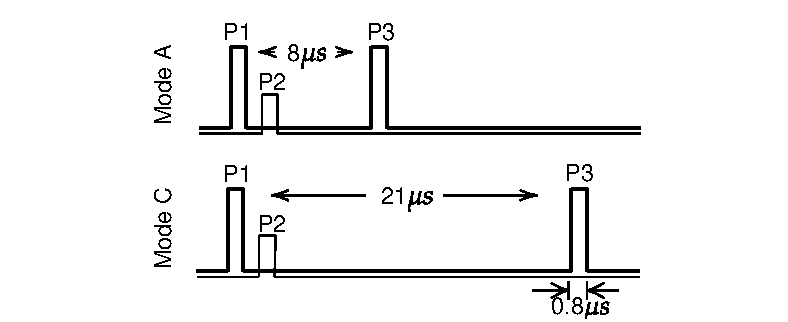
\includegraphics[scale=0.8]{figures/intro/mode_ac_uplink_pulses.pdf}
  \caption{Mode~A/C interrogation pulses}
  \label{fig:mode_ac_uplink_pulses}
\end{figure}

The pulses are about 0.8 microseconds wide. P1 and P3 are the two main pulses sent by the directional antenna. They are separated by 8 microseconds and 21 microseconds respectively for Mode~A and C. P2 is a pulse sent by the omnidirectional antenna right after P1. Pulse P2 is introduced for sidelobe suppression. When the aircraft is close to the radar, the power of P2 can be higher than P1. In this case, the interrogation is likely generated by the side lobes of the directional antenna and should be ignored by the aircraft.

In Figure \ref{fig:mode_ac_downlink_pulses}, an example of a Mode~A/C reply is shown. Each reply consists of two persistent pulses separated by 20.3 microseconds (F1 and F2). Within this period, either the identity code or the altitude code is encoded using 13 0.45 microseconds pulses. The pulses are separated by gaps of one microsecond. The pulse at the center serves as a verification pulse and is always absent. The presence or absence of any other 12 pulses represents a 1 or 0 bit. When required by air traffic controllers for identification purposes, a special purpose identification (SPI) may follow F2 after two absent pulses.

\begin{figure}[ht]
  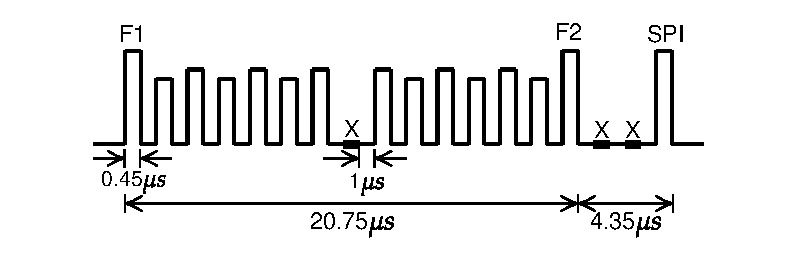
\includegraphics[scale=0.8]{figures/intro/mode_ac_downlink_pulses.pdf}
  \caption{Mode~A/C interrogation pulses}
  \label{fig:mode_ac_downlink_pulses}
\end{figure}

The response type (A or C) cannot be identified based on the reply signal itself. The SSR determines the content based on the synchronization with interrogations. This design of ATCRBS works sufficiently well with low-density air traffic, but it cannot efficiently cope with higher flight densities since all aircraft replies are transmitted on the same frequency. When several aircraft are in the same direction of the radar beam, reply signals can overlap and introduce errors for decoding. This is known as synchronous garbling.

When there are multiply secondary radars in the vicinity, replies originated by other radars may be considered as valid responses of one radar, which in turn, causes errors and confusion. This syndrome is called FRUIT (False Replies Unsynchronized In Time).

Though some of the garbling and the FRUIT problem can be mitigated with the reduction of interrogation frequency and improvements in signal processing ability, the information transmitted in Mode~A and Mode~C is still very limited. The number of identity codes available in Mode~A communication is limited to a maximum of 4096 unique codes, which poses another clear limitation.

Hence, more advanced communication protocols needed to be developed to acquire more information from a large number of aircraft.



\section{Mode~S}

Mode~S (Mode~Select Beacon System) was designed by Lincoln Laboratory at Massachusetts Institute of Technology in the 1970s. Based on different iterations of hardware and software design in the 1980s, the implementation of Mode~S in air traffic control began in the 1990s. Since then, Mode~S has become one of the main sources for aircraft surveillance.

The main characteristic of Mode~S is its selective interrogation, which allows the SSR to interrogate different information from different aircraft separately. By using selective interrogation, it largely mitigated the problem of garbling in Mode~A/C and thus greatly improved the capacity of the communication channel.

Unlike the limited number (4096) of unique identification codes in Mode~A communication, the Mode~S transponder is identified by a 24-bit transponder code, which can support up to 16,777,216 ($2^{24}$) unique addresses. In addition to these two major advantages, the Mode~S protocol introduced many different types of information that could be interrogated and downlinked.

\subsection{Mode~S interrogations}
The Mode~S uplink signal contains parameters that indicate which information is desired by the air traffic controller. There are two types of Mode~S interrogations, which are shown in Figure \ref{fig:mode_s_uplink_pulses}. The short interrogation has 56 bits of information contained in the data block, while the long interrogation contains 112 bits of information. The P2 pulse acts as the sidelobe suppression for Mode~A/C transponders so that they will ignore the rest of the interrogation pulses. Information in the Mode~S interrogation data block is uses the Differential Phase-Shift Keying (DPSK) modulation \cite{mazda2014}.

\begin{figure}[ht]
  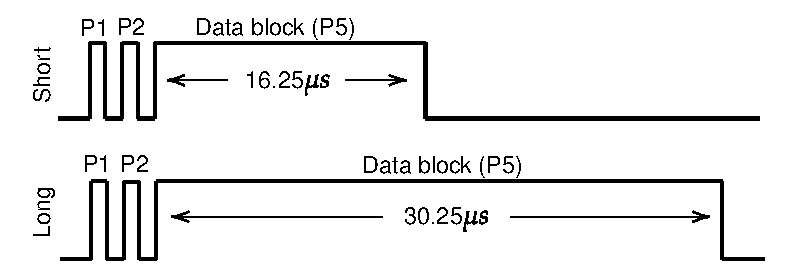
\includegraphics[scale=0.8]{figures/intro/mode_s_uplink_pulses.pdf}
  \caption{Mode~S uplink pulses}
  \label{fig:mode_s_uplink_pulses}
\end{figure}


\subsection{Mode~S replies}
There two types of Mode~S downlink signals, short reply and long reply, which correspond to the short and long interrogations from the SSR. For each microsecond, two bits are transmitted. All Mode~S replies start with an 8-microsecond fixed preamble and continue with 56 or 122 microseconds for the data block. The structure of the downlink message is shown in Figure \ref{fig:mode_s_downlink_pulses}.

\begin{figure}[ht]
  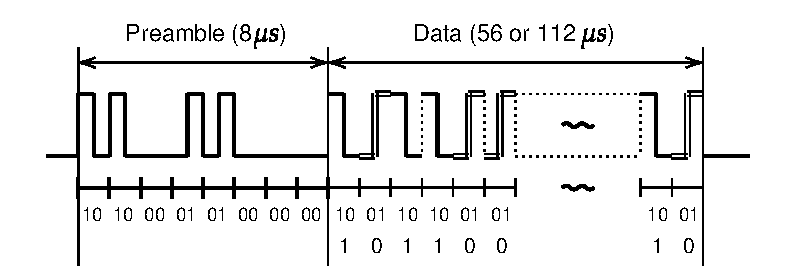
\includegraphics[scale=0.8]{figures/intro/mode_s_downlink_pulses.pdf}
  \caption{An example of Mode~S reply message}
  \label{fig:mode_s_downlink_pulses}
\end{figure}

The 16-bit fix preamble can be represented as \texttt{1010000101000000} in binary. The information contained in the data block is modulated using the Pulse Position Modulation (PPM), which is a type of amplitude modulation. In PPM, the \1 bit is represented by a 0.5-microsecond of pulse followed by a 0.5-microsecond flat signal. The \0 bit is reversed compared to the \1 bit. It is represented by a 0.5-microsecond flat signal and followed by a 0.5-microsecond pulse.

\begin{notebox}{Note}
  Mode~S uplink and downlink signals use different modulation methods. The uplink uses phase modulation, while the downlink uses amplitude modulation. Phase modulation requires slightly more complicated hardware implementation but has a better performance in terms of error tolerance. 
\end{notebox}

\subsection{Compatibility with Mode~A/C}

Similar to Mode~A/C, Mode~S SSR can send \emph{All-Call} interrogations to all aircraft in the vicinity. The All-Call interrogations are designed to be compatible with Mode~A/C transponders. In Figure \ref{fig:mode_s_all_call}, the All-Call interrogation is shown. There is an 8 or 21 microseconds between P1 and P3, which is the same as Mode~A/C. P4 is a wider pulse lasting for 1.6 microseconds.

\begin{figure}[ht]
  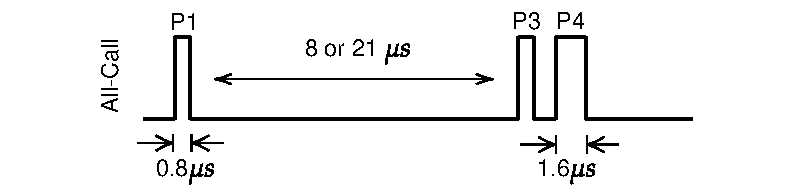
\includegraphics[scale=0.8]{figures/intro/mode_acs_all_call.pdf}
  \caption{Mode~A/C/S All-Call interrogation}
  \label{fig:mode_s_all_call}
\end{figure}

When a Mode~A/C transponder receives this interrogation, the last pulse P4 is ignored. Hence, a normal Mode~A or Mode~C reply is replied. A Mode~S transponder would detect P4, and thus, produce a Mode~S All-Call reply. The Mode~A/C/S All-Call reply is designed for SSR to identify which aircraft are in the vicinity, including Mode~A/C only aircraft.

This is one of the several different interrogation pulse patterns from a Mode~A/C compatible Mode~S radar. Most current SSRs can perform both Mode~A/C and Mode~S interrogations. In Figure \ref{fig:mode_s_inter_mode}, the interrogation pulses and replies from aircraft transponders are summarized.

\begin{figure}[ht]
  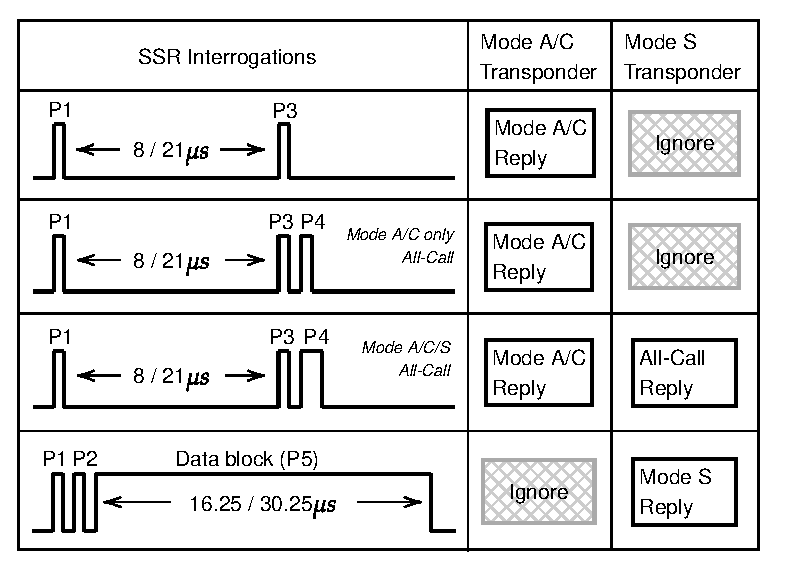
\includegraphics[scale=0.8]{figures/intro/mode_s_inter_mode.pdf}
  \caption{SSR interrogations pulses and transponder replies}
  \label{fig:mode_s_inter_mode}
\end{figure}

We can see that:

\begin{itemize}
  \item Mode~A/C transponders respond to all interrogations with P1 and P3.
  \item When P4 is not present or a shorter P4 is used (as shown in the first and second patterns), Mode~S transponders will ignore the interrogations.
  \item Mode~S transponders will produce an All-Call reply to interrogations with a long P4. This interrogation is used to acquire all aircraft with either Mode~A/C or Mode~S capability.
  \item Finally, all Mode~S interrogation is designed to be ignored by Mode~A/C transponders due to the presence of P2 (as shown in the last pattern), which is considered as a side lobe suppression mechanism for Mode~A/C transponders.
\end{itemize}


\begin{notebox}{Note}
  Mode~S SSR is also able to produce a Mode~S only All-Call interrogation using the standard Mode~S uplink (with uplink format 11).
\end{notebox}


\subsection{Mode~S format}

The Mode~S communication protocol is designed to handle different types of uplink and downlink message formats. The first 5 bits of the uplink or downlink message define the uplink format (UF) or downlink format (DF) number of the message. Based on the UF/DF number, different structures of the data block are defined. In Table \ref{tb:mode_s_formats}, all available Mode~S formats are shown. Currently, 11 Mode~S formats are being used. Numbers not in this table are reserved for future use.

\begin{table}[ht]
\centering
\footnotesize
\caption{Mode~S uplink and downlink formats}
\label{tb:mode_s_formats}
\begin{tabular}{|l|l|l|l|}
\hline
\textbf{UF/DF} & \textbf{Bits} & \textbf{Uplink type} & \textbf{Downlink type} \\ \hline\hline
0 & 56 & Short air-air surveillance (ACAS) & Short air-air surveillance (ACAS) \\ \hline
4 & 56 & Surveillance, altitude request & Surveillance, altitude reply \\ \hline
5 & 56 & Surveillance, identity request & Surveillance, identity reply \\ \hline
11 & 56 & Mode~S All-Call & All-Call reply \\ \hline
\hline
16 & 112 & Long air-air surveillance (ACAS) & Long air-air surveillance (ACAS) \\ \hline
17 & 112 & - & Extended squitter \\ \hline
18 & 112 & - & Extended squitter / non transponder \\ \hline
19 & 112 & - & Military extended squitter \\ \hline
20 & 112 & Comm-A, altitude request & Comm-B, altitude reply \\ \hline
21 & 112 & Comm-A, identity request & Comm-B, identity reply \\ \hline
24 & 112 & Comm-C (ELM) & Comm-D (ELM) \\ \hline
\end{tabular}
\end{table}


\begin{notebox}{Note}
  Format number 24 is an exception. It is identified using only the first two bits, which must be \texttt{11}. All following bits are used for encoding other information.
\end{notebox}


We can see that the short 56-bit data block is used to encode messages with format numbers from 0 to 11. Messages with format numbers above 16 are encoded with the long 112-bit data block. Among all uplink formats, UF 17, 18, and 19 are not used. This is because the corresponding downlink messages (extended squitter messages) are designed to be broadcast automatically without the need for SSR interrogations. 

One of the most common applications for the extended squitter is the Automatic Dependent Surveillance-Broadcast service, which is also commonly known as ADS-B.


\section{ADS-B}

Automatic Dependent Surveillance-Broadcast (ADS-B) is a surveillance technology designed to allow aircraft to broadcast their flight state periodically without the need for interrogation. The word \emph{automatic} refers to the fact that no inputs from controllers or pilots are required. The word \emph{dependent} indicates this technology depends on information from other onboard systems, such as air data systems and navigation systems.

Common aircraft state parameters included in ADS-B are position, altitude, and speed. The position is determined by Global Navigation Satellite Systems (GNSS). The velocity is derived from the GNSS position and the inertial measurement system. The altitude information includes both barometric altitude and GNSS altitude. The barometric altitude is provided by the air data system. In addition to these primary state parameters, ADS-B also allows other information to be broadcast, for example, aircraft call-sign, accuracy indicators, integrity indicators, and operational status.

Different types of ADS-B messages are identified by Type Codes. The structures of these messages are all defined in ICAO documents, such as in \cite{icao9871v1} and \cite{rtca2011mops}. In Part I of this book, we will explain how these different types of ADS-B messages can be decoded.

\begin{notebox}{Note}
Originally, there were three candidates to build ADS-B: Mode~S Extended Squitter, VHF Data Link - Mode~4 (VDL4), and Universal Access Transceiver (UAT). Different specifications are designed for these frequency channels \cite{rtca2011mops, rtca2002uat}. However, the Mode~S extended squitter implementation of ADS-B is the most adopted one among all candidates. UAT is only partially implemented in some countries like the USA, while VDL4 did not go beyond the test phase.
\end{notebox}


\section{Other Mode~S services}

The most common data format number used in Mode~S for information downlink are 4, 5, 20, and 21. Format 4 and 5 are short messages designed to acquire aircraft altitude and identity (similar to Mode~A/C messages). Downlink messages with format 20 or 21, as known as Comm-B messages, contain other information desired by air traffic controllers, in addition to altitude and identity.

In theory, up to 255 different message types are supported by the Mode~S Comm-B. A new parameter, Comm-B Data Selector (BDS), is designed to identify which additional information is included in Mode~S messages. It functions similarly to the Type Code of ADS-B message. In practice, not all 255 BDS codes are defined or used. 

A subgroup of these codes is commonly interrogated by air traffic controllers. By combining different BDS codes into groups, several Mode~S services are defined. The two most used services are Mode~S Elementary Surveillance (ELS) and Mode~S Enhanced Surveillance (EHS) \cite{grappel2008}. For example, in the European airspace, aircraft above certain take-off weight category are required to have these capabilities enabled.

The Mode~S Elementary Surveillance (ELS) consists of four BDS codes (10, 17, 20, and 30). It provides basic information such as Mode~S capabilities, identification (callsign), and ACAS resolution advisory, in addition to the altitude or identity (squawk code) information. 

The Mode~S Enhanced Surveillance consists of three BDS codes (40, 50, and 60). It provides much more additional information on aircraft states, such as selected altitudes, true airspeed, indicated airspeed, Mach number, bank angle, and turn rate.

In addition to the common ELS and EHS, the meteorological routine air report (MRAR), and the meteorological hazard report (MHR) are also interrogated in some controlled airspaces. These reports provide weather-related information such as wind and temperature that are measured by the aircraft sensors.


\section{Summary}

In Figure \ref{fig:mode_s_services}, all aforementioned Mode~S services and their relationships with Mode~S downlink formats are illustrated.

\begin{figure}[ht]
  \centering
  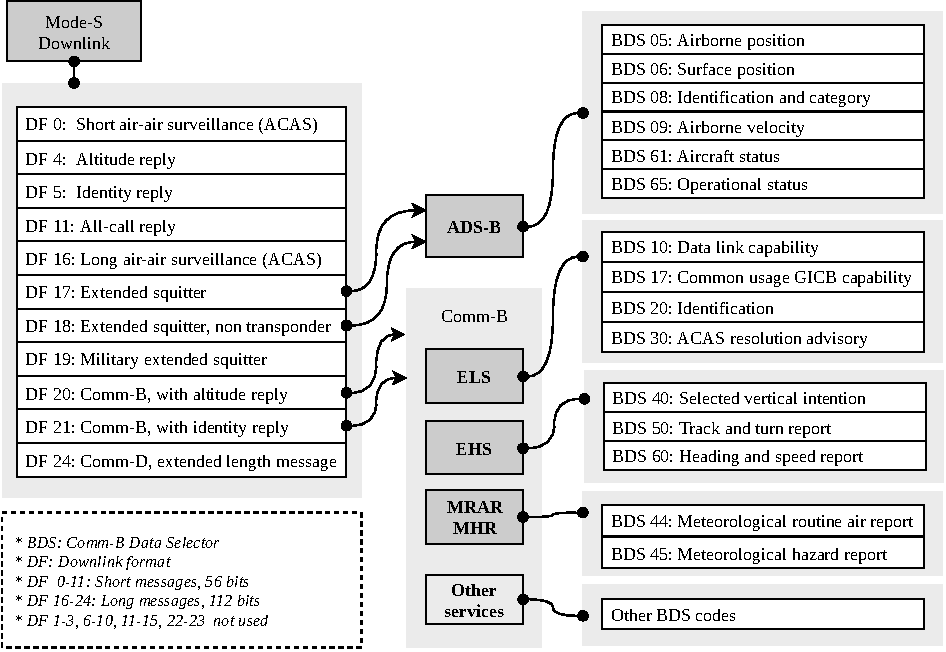
\includegraphics[width=\textwidth]{figures/intro/mode_s_services.pdf}
  \caption{Relationship between Mode~S downlink formats and different services}
  \label{fig:mode_s_services}
\end{figure}

In the rest of this book, the details of these services are discussed in different chapters. In chapter 2 (the rest of Part I), common hardware and software setups are shown. In chapter 3 to 10 (Part II), the focus is on ADS-B messages. Detailed guides on how to decode different types of messages are presented. In chapter 11 to 19 (Part III), the focus is on Mode~S ELS, EHS, and meteorological services. Accordingly, the decoding and inference of the messages are provided.

\chapter{Quick Start: Hardware and Software to Receive Mode~S Signals}
\label{chap:quickstart}

Chapter 1 introduced several fundamental concepts about Mode~S communication. This chapter focuses on the practical aspects of Mode~S data, specifically, how to receive and obtain information that is transmitted in Mode~S downlink communications. Mode~S signals are transmitted using 1090 MHz radio waves. Hence, the receiver and antenna have to be designed to work with this frequency. Nowadays, all necessary components required to obtain the Mode~S data can be easily made with low-cost off-the-shelf components. Several open-source software tools are available to support the extraction and decoding of data from Mode~S signals. In this chapter, we explain how to step up a functional hardware and software system to receive Mode~S data.

\section{Range}
Since Mode~S uses L band signals that follow the line-of-sight propagation, any obstructions between the transmitter and receiver can cause a significant amount of signals to be blocked. Assuming that no obstacle exists between the aircraft and the receiver, and the transmitter has a sufficient amount of power, the maximum range of the receiver is determined by the curvature of the earth. Figure \ref{fig:max_range} illustrates how the maximum range of the receiver can be obtained.

\begin{figure}[ht]
\centering
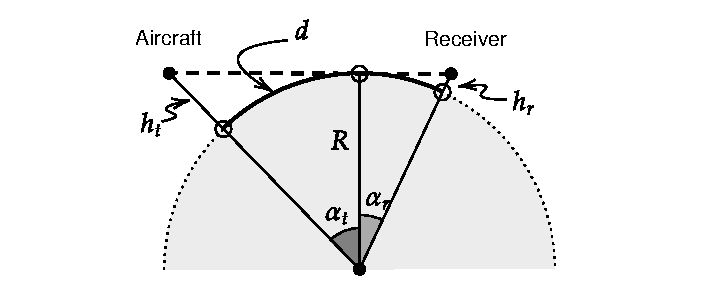
\includegraphics[scale=0.9]{figures/quickstart/max_range.pdf}
\caption{Maximum receiver range}
\label{fig:max_range}
\end{figure}


Knowing the altitude of the receiver antenna, it is possible to determine the maximum range ($d$) of a Mode~S receiver as:

\begin{align}
  d &= (\alpha_r + \alpha_t) R \\
  & = \left( \arccos \frac{R}{R+h_r} + \arccos \frac{R}{R+h_t} \right) R
\end{align}

\noindent where $R$ is the radius of the earth, while $h_t$ and $h_r$ are the height of the aircraft and receiver above the sea level. Using this equation, we can calculate the maximum receiving range for aircraft flying at different altitudes. Figure \ref{fig:max_range_curve} shows the maximum range curves calculated using several receiver heights.

\begin{figure}[ht]
  \centering
  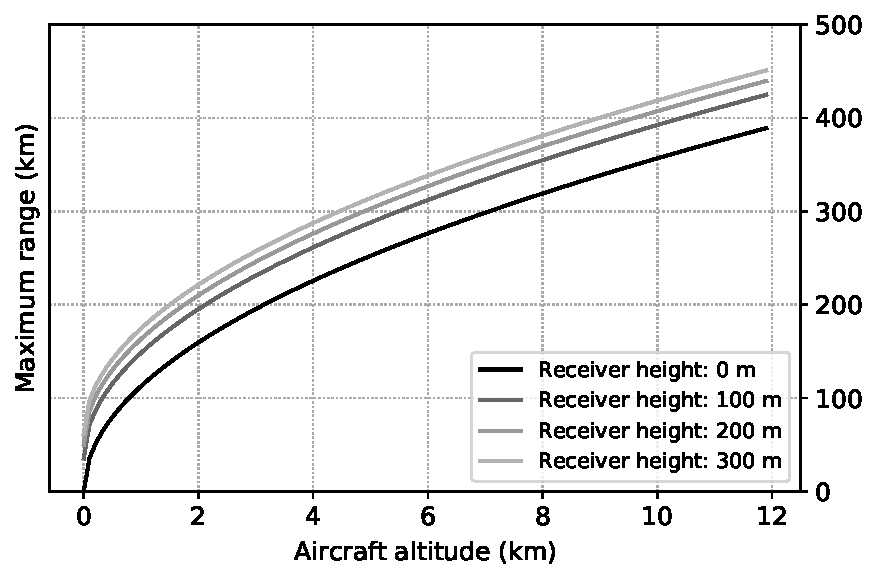
\includegraphics[scale=0.65]{figures/quickstart/max_range_curve.pdf}
  \caption{Maximum receiver range curve}
  \label{fig:max_range_curve}
\end{figure}


It should be noted that this figure shows the maximum radio range due to the curvature of the Earth. However, in real-life applications, Mode~S signal follows the Friis transmission model, which states that the maximum distance also depends on the power of the transmitter, as well as the directivities of the transmission and receiving antennas. When considering these factors, the actual radio range for the receiver is typically lower than the theoretical values shown in the previous figure.

\section{Antenna}
In principle, any antenna designed for the radio frequency around 1 GHz can be used for receiving Mode~S signals. A large variety of commercial off-the-shelf antennas can be found nowadays. 

However, it is not difficult to design your own antenna. The carrier frequency of Mode~S is 1090 MHz, which corresponds to the wavelength of 27.5 centimeters. In order to have an antenna that is tuned to this specific frequency, one can design the antenna simply using a piece of a conductor (metal wire) and a coaxial feeder cable. Figure \ref{fig:antennas} shows a few common antenna designs.

\begin{figure}[ht]
  \centering
  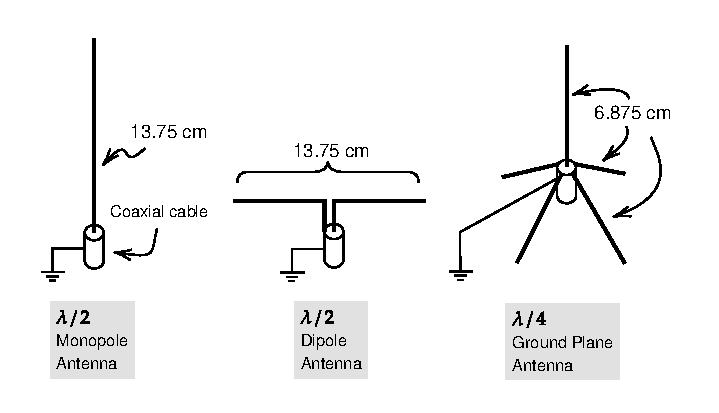
\includegraphics[scale=0.95]{figures/quickstart/antennas.pdf}
  \caption{Common antenna designs}
  \label{fig:antennas}
\end{figure}

The monopole antenna and the dipole antenna both are half-wavelength ($\lambda/2$) antennas with a total conductor length of 13.75 cm. The ground plane antenna is a quarter-wavelength ($\lambda/4$) antenna, where the main pole is 6.875 cm.

All these previous antennas are omnidirectional. Some time is also desirable to make use of directional antennas (such a Yagi antenna), for example, to receive messages coming from the airport direction with a higher receiving gain.

For a remote installation where the antenna is far from the receiver (i.e., long coaxial cable between the antenna and receiver), the high-frequency signal of Mode~S can attenuate quickly. When the signal has arrived at the receiver end, the signal-to-noise ratio can become quite high. To overcome this limitation, an active antenna may be used.

The active antenna (see Figure \ref{fig:biastee_active_antenna}) has a low-noise amplifier integrated on the antenna side. Sometimes, it also includes a band-pass filter that is designed for 1090 MHz. The active antenna requires additional powering. Power is commonly supplied through a bias-tee device connected at the receiver end, which is on the left-hand side of the diagram. On the right-hand side, the radio frequency is mixed with the DC component, which allows the electronic circuit to be powered close to the receiver end.

\begin{figure}[ht]
  \centering
  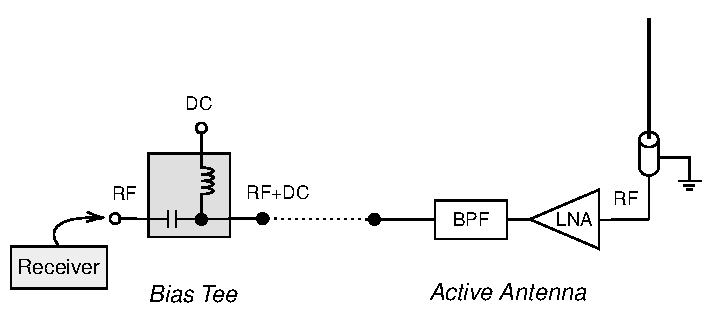
\includegraphics[scale=0.9]{figures/quickstart/biastee_active_antenna.pdf}
  \caption{Diagram of an active antenna powered through a bias-tee}
  \label{fig:biastee_active_antenna}
\end{figure}


\section{Receiver}

Many modern Mode~S receivers are built using software-defined radio (SDR). An SDR usually can be tuned to a wide range of radio frequencies. The user can conveniently select the center frequency of the receiver and the sampling rate, as well as defined the bandwidth of the onboard low-pass filter if it is supported.

For receiving ADS-B (and other types of Mode~S message), a RTL-SDR is the most common type of low-cost receiver to choose. Many different brands of RTL-SDR receivers exist; they are often built with the Realtek RTL2832U chipset. It can work with radio frequencies from 24 to 1766 MHz. The maximum sampling rate is 2.8 million samples per second (MSPS). Given that a Mode~S bit consists of a pulse cycle of 0.5 {\textmu}s (see Figure \ref{fig:mode_s_uplink_pulses}), the minimum SDR sampling rate required for Mode~S is 2 MSPS. RLT-SDR devices just barely manage to meet this requirement.

\begin{notebox}{Note}
  The maximum frequency range of RTL-SDR can be from 0 to 2220 MHz. However, the sensitivity drops off significantly outside the 24 -- 1766 MHz range. The sampling rate can actually go up to a maximum of 3.2 million samples per second, but some samples may be dropped at this sampling rate. So, it is not stable.
\end{notebox}

SDRs that offer a higher performance also exist. They often support a larger frequency range with higher sampling rates. Some offer multiple transmitting (TX) and receiving (RX) channels. Table \ref{tb:sdr} lists a few examples of common SDR devices. The performance of RTL-SDR is listed as a comparison.

\begin{table}[ht]
  \footnotesize
  \caption{Examples of common software defined radio devices}
  \label{tb:sdr}
  \begin{tabular}{|l|l|l|l|l|l|}
  \hline
   & \textbf{RTL-SDR} & \textbf{AirSpy R2} & \textbf{HackRF 1} & \textbf{LimeSDR} & \textbf{BladeRF 2} \\ \hline
  \textbf{Frequency (from)} & 24 MHz & 24 MHz & 1 MHz & 100 KHz & 47 MHz \\ \hline
  \textbf{Frequency (to)} & 1766 MHz & 1700 MHz & 6000 MHz & 3800 MHz & 6000 MHz \\ \hline
  \textbf{Max sample rate} & 2.8 MSPS & 10 MSPS & 20 MSPS & 61.44 MSPS & 61.44 MSPS \\ \hline
  \textbf{RX channels} & 1 & 1 & 1 & 2 & 2 \\ \hline
  \textbf{TX channels} & 0 & 1 & 1 & 2 & 2 \\ \hline
  \textbf{Open hardware} & No & Partially & Full & Full & Partially \\ \hline
  \end{tabular}
\end{table}

\section{Software tools}

Several software tools are also available to work with some of these SDR devices and decode Mode~S and ADS-B signals directly. In this section, we explain how to use two open-source tools, which are \texttt{dump1090} and \texttt{pyModeS}.

\subsection{dump1090}

\texttt{dump1090} is the most well-known open-source Mode~S decoder currently available. The software is written in C programming language and was originally developed by Salvatore Sanfilippo \footnote{https://github.com/antirez/dump1090} under the BSD-3-Clause license.

Since its release in 2013, the repository has been forked and extended intensively on GitHub, creating more than 900 forks so far. Many of the branched versions contain different variations, such as support for additional hardware, additional decoded Mode~S messages, and additional output format. Currently, one of the most comprehensive forks is the repository maintained by FlightAware.\footnote{https://github.com/flightaware/dump1090} The following examples will be based on the FlightAware version of \texttt{dump1090}, using a Debian-based Linux system.

\subsubsection{Installation of dump1090}
The latest version of \texttt{dump1090} source code can download as follows:

\begin{verbatim}
$ git checkout https://github.com/flightaware/dump1090.git
\end{verbatim}

Before compiling the code, following dependencies must be installed:

\begin{verbatim}
sudo apt-get install build-essential debhelper librtlsdr-dev \
  pkg-config dh-systemd libncurses5-dev libbladerf-dev
\end{verbatim}

Next, we can compile the source code as:

\begin{verbatim}
$ cd dump1090
$ make
\end{verbatim}

It is worth noting that the FlightAware version of \texttt{dump1090} supports both RTL-SDR and BladeRF devices by default.

\subsubsection{Default usage of dump1090}

Once it is compiled and the RTL-SDR receiver is connected, we can run the following command to start receiving and decoding signals:

\begin{verbatim}
$ ./dump1090
\end{verbatim}

With the default option, Mode~S messages and decoded information are displayed in the terminal. For example:

\begin{verbatim}
*8d451dbd9905b5018004005979c5;
CRC: 000000
RSSI: -20.6 dBFS
Score: 1800
Time: 9214131.08us
DF:17 AA:451DBD CA:5 ME:9905B501800400
 Extended Squitter Airborne velocity over ground, subsonic (19/1)
  ICAO Address:  451DBD (Mode~S / ADS-B)
  Air/Ground:    airborne
  Ground track   271.4
  Groundspeed:   436.1 kt
  Geom rate:     0 ft/min
  NACv:          0
\end{verbatim}

\subsubsection{Raw Mode~S messages}

If we only want to display the  raw messages, the \texttt{----raw} option can be provided, as follows:

\begin{verbatim}
$ ./dump1090 --raw
\end{verbatim}

In this case, the terminal output will only contain the raw messages, for example:

\begin{verbatim}
*5d4074358ad00c;
*8d407435990dbd01900484f66c3c;
*8d40743558af828cd326fe0c2fe9;
*a80011b1e0da112fe0140060939f;
*a00015b8c2680030a80000318667;
*5d4074358ad030;
*5d4074358ad030;
\end{verbatim}

\subsubsection{Interactive mode}

\texttt{dump1090} can also provide a live view of all aircraft seen by the receiver through the use of the \texttt{----interactive} option:

\begin{verbatim}
$ ./dump1090 --interactive
\end{verbatim}

An example of the terminal output is shown in Figure \ref{fig:dump1090}.

\begin{figure}[ht]
  \centering
  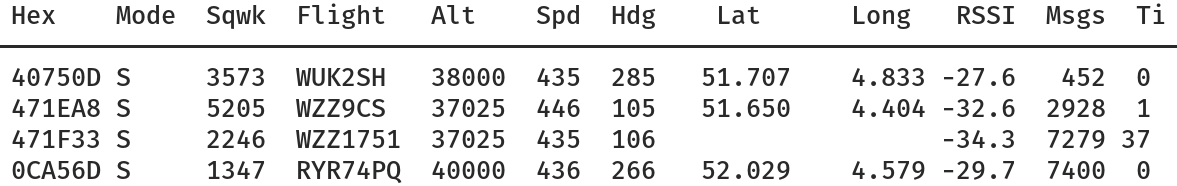
\includegraphics[scale=0.33]{figures/quickstart/dump1090.png}
  \caption{Example of a dump1090 interactive output}
  \label{fig:dump1090}
\end{figure}


% An example of the terminal output for the interactive view is shown as follows:

% \begin{verbatim}
% Hex    Mode~Sqwk Flight  Alt    Spd  Hdg   Lat    Long   RSSI   Msgs  Ti
% ------------------------------------------------------------------------
% 40750D S    3572 WUK2SH  38000  435  285  51.707  4.833  -27.6   452   0
% 471EA8 S    5205 WZZ9CS  37025  446  105  51.650  4.404  -32.6  2928   1
% 471F33 S    2246 WZZ1751 37025  435  106                 -34.3  7279  37
% 0CA56D S    1347 RYR74PQ 40000  436  266  52.029  4.579  -29.7  7400   0
% \end{verbatim}
  


\subsection{pyModeS}
\texttt{pyModeS} is an open-source Mode~S decoder project that I started in 2015. It is a library that was originally designed to focus on lower level inference and decoding of individual raw Mode~S messages. Later on, hardware support and live decoding were added, which made it more akin to \texttt{dump1090} of late.

\begin{notebox}{Note}
  Some technical terms related to ADS-B and Mode~S are used in this section. They will be explained in detail in later chapters.
\end{notebox}

\subsubsection{Installation of pyModeS}

As a Python library, it is possible to install the most recent stable version of \texttt{pyModeS} as:

\begin{verbatim}
pip install --upgrade pyModeS
\end{verbatim}

The latest development version for the GitHub can be installed as:

\begin{verbatim}
pip install --upgrade git+https://github.com/junzis/pyModeS
\end{verbatim}


\subsubsection{Live traffic view}

\texttt{pyModeS} provides the possibility to view live traffic through the \texttt{modeslive} command. The usage of this command is shown as follows:

\begin{verbatim}
$ modeslive [-h] --source SOURCE [--connect SERVER PORT DATAYPE]
            [--latlon LAT LON] [--show-uncertainty] [--dumpto DUMPTO]

arguments:
 -h, --help            Show this help message and exit
 --source SOURCE       Choose data source, "rtlsdr" or "net"
 --connect SERVER PORT DATATYPE
                       Define server, port and data type. Supported data
                       types are: ['raw', 'beast', 'skysense']
 --latlon LAT LON      Receiver latitude and longitude, needed for the surface
                       position, default none
 --show-uncertainty    Display uncertainty values, default off
 --dumpto DUMPTO       Folder to dump decoded output, default none
\end{verbatim}

When an RTL-SDR device is connected, the following command can be used to display live traffic:

\begin{verbatim}
$ modeslive --source rtlsdr
\end{verbatim}

Data source can also be supplied through the network (for example, from \texttt{dump1090} TCP output stream) as:



\begin{verbatim}
$ dump1090 --net --quiet
$ modeslive --source net --connect localhost 30002 raw
\end{verbatim}

An example of the live view is shown in Figure \ref{fig:modeslive}.

\begin{figure}[ht]
  \centering
  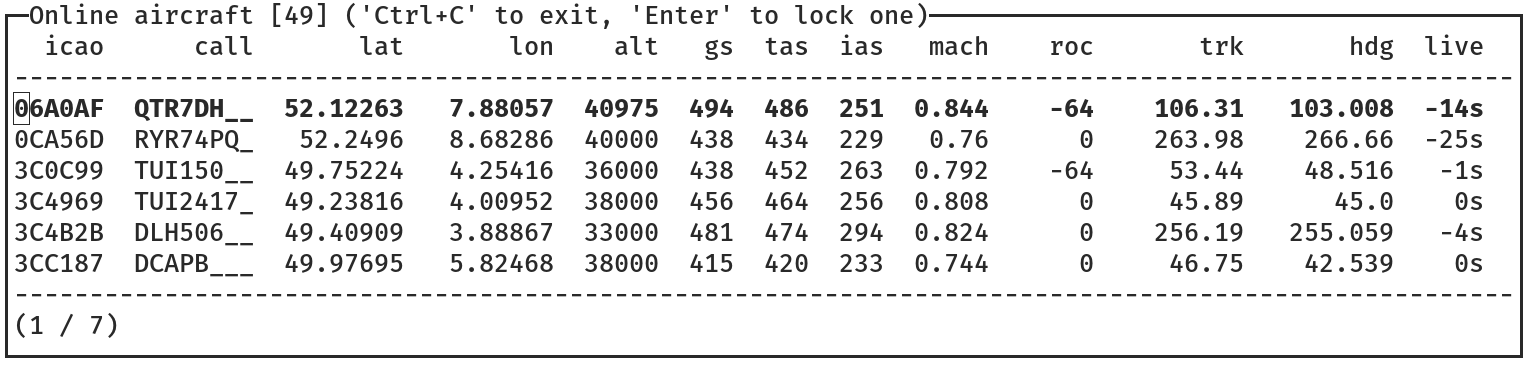
\includegraphics[scale=0.3]{figures/quickstart/modeslive.png}
  \caption{Example of a live view of \texttt{modeslive} from \texttt{pyModeS}}
  \label{fig:modeslive}
\end{figure}

Real-time flight states are shown, including, for example, ICAO transponder code, call sign, position,  altitude, ground speed, true airspeed, indicated airspeed, Mach number, rate of climb, track angle, and heading.

\subsubsection{Programming interface}

Since \texttt{pyModeS} is originally designed as a library aimed for research, and thanks to the use of Python programming language, one can easily make use of its low-level decoding functionalities.

For example, core functions of \texttt{pyModeS} can be used to decode Downlink Format, ICAO address, ADS-B Type Code, as well as to perform parity check:

\begin{verbatim}
import pyModeS as pms

pms.df(msg)         # Downlink Format
pms.icao(msg)       # Infer the ICAO address from the message
pms.crc(msg)        # Perform parity check
pms.typecode(msg)   # Obtain ADS-B message Type Code
\end{verbatim}


ADS-B related functions allow information such as identity, position, and velocities to be decoded. For example:

\begin{verbatim}
# position messages
pms.adsb.position(msg_even, msg_odd, t_even, t_odd)
pms.adsb.altitude(msg)

# velocity messages
pms.adsb.velocity(msg)
\end{verbatim}

There are also a number of functions designed to infer and decode Mode~S downlink messages. For example:

\begin{verbatim}
# Mode S altitude code (DF=4/20)
pms.common.altcode(msg)

# Mode S squwak code (DF=5/21)
pms.common.idcode(msg)

# Infer Modes S BDS code
pms.bds.infer(msg)

# BDS 4,0
pms.commb.selalt40mcp(msg)  # MCP/FCU selected altitude (ft)
pms.commb.selalt40fms(msg)  # FMS selected altitude (ft)
pms.commb.p40baro(msg)      # Barometric pressure setting (mb)

# BDS 5,0
pms.commb.roll50(msg)       # Roll angle (deg)
pms.commb.trk50(msg)        # True track angle (deg)
pms.commb.gs50(msg)         # Ground speed (kt)
pms.commb.rtrk50(msg)       # Track angle rate (deg/sec)
pms.commb.tas50(msg)        # True airspeed (kt)

# BDS 6,0
pms.commb.hdg60(msg)        # Magnetic heading (deg)
pms.commb.ias60(msg)        # Indicated airspeed (kt)
pms.commb.mach60(msg)       # Mach number (-)
pms.commb.vr60baro(msg)     # Barometric altitude rate (ft/min)
pms.commb.vr60ins(msg)      # Inertial vertical speed (ft/min)
\end{verbatim}

These are commonly used functions related to Mode~S decoding. A complete list of the APIs can be found in the \texttt{pyModeS} library API documentation. In the rest of this book, most of the decoding details are explained, which will often involving the use of \texttt{pyModeS} and reflect its source code.


\part{Decoding ADS-B}
\chapter{ADS-B Basics} \label{chap:adsb-basic}
ADS-B is short for Automatic Dependent Surveillance-Broadcast. It is a satellite-based surveillance system. Parameters such as position, velocity, and identification are transmitted through Mode~S Extended Squitter (1090 MHz). Nowadays, the majority of the aircraft are broadcasting ADS-B messages constantly.

\section{Message structure}

An ADS-B frame is 112 bits long and consists of 5 main parts, as follows:

\begin{verbatim}
+----------+----------+-------------+------------------------+-----------+
|  DF (5)  |  CA (3)  |  ICAO (24)  |         ME (56)        |  PI (24)  |
+----------+----------+-------------+------------------------+-----------+
\end{verbatim}

Any ADS-B message must start with the Downlink Format 17. In case of a TIS-B message, the Downlink Format is 18. They correspond to 10001 or 10010 in binary for the first 5 bits. Bits 6-8 are used as an additional identifier, which presents different meanings within each ADS-B subtype.

In Table \ref{tb:adsb-structure}, the key information of an ADS-B message is listed.

\begin{table}[!ht]
\centering
\caption{Structure of ADS-B frame}
\label{tb:adsb-structure}
\begin{tabular}{|l|l|l|l|}
\hline
\textbf{Bit} & \textbf{No. bits} & \textbf{Abbreviation} & \textbf{Information} \\ \hline\hline
1-5 & 5 & DF & Downlink Format \\ \hline
6-8 & 3 & CA & Transponder capability \\ \hline
9-32 & 24 & ICAO & ICAO aircraft address \\ \hline
33-88 & 56 & ME & Payload message \\
(33-37) & (5) & (TC) & (Type code) \\ \hline
89-112 & 24 & PI & Parity/Interrogator ID \\ \hline
\end{tabular}
\end{table}

It is worth noting that the ADS-B Extended Squitter sent from a Mode~S transponder uses Downlink Format 17 (\texttt{DF=17}). Non-Transponder-Based ADS-B Transmitting Subsystems and TIS-B Transmitting equipment use Downlink Format 18 (\texttt{DF=18}). By using \texttt{DF=18} instead of \texttt{DF=17}, an ADS-B/TIS-B Receiving Subsystem will know that the message comes from equipment that cannot be interrogated.

\section{Capability}

The second field consists of three bits that indicate the transponder level. The capability value can be between 0 and 7. The definitions of these values are shown in Table \ref{tb:transponder_capability}.

\begin{table}[!ht]
\centering
\caption{Mode~S transponder capability (CA)}
\label{tb:transponder_capability}
\begin{tabular}{|l|p{10cm}|}
\hline
\textbf{CA} & \textbf{Definition} \\ \hline
0 & Level 1 transponder \\ \hline
1-3 & Reserved \\ \hline
4 & \makecell*{Level 2+ transponder, \\ with ability to set CA to 7, \\ on-ground} \\ \hline
5 & \makecell*{Level 2+ transponder, \\ with ability to set CA to 7, \\ airborne} \\ \hline
6 & \makecell*{Level 2+ transponder, \\ with ability to set CA to 7, \\ either on-ground or airborne} \\ \hline
7 & \makecell*{Signifies the Downlink Request value is 0, \\ or the Flight Status is 2, 3, 4 or 5, \\ either airborne or on the ground} \\ \hline
\end{tabular}
\end{table}

\section{ICAO address}

In each ADS-B message, the sender (originating aircraft) can be identified using the Mode~S transponder address assigned accordingly ICAO regulations. Very often this is referred as ICAO address. 

The ICAO address is located from 9 to 32 bits in binary (or 3 to 8 in hexadecimal positions). A unique ICAO address is assigned to each Mode~S transponder of an aircraft and serves as the unique identifier for each aircraft.


\section{ADS-B message types}

To identify what information is contained in an ADS-B message, we need to take a look at the Type Code of the message, indicated at bits 33 - 37 (or first 5 bits of the \texttt{ME} segment).

In following Table \ref{tb:adsb-tc}, the relationships between each Type Code and its information contained in the \texttt{ME} segment are shown.

\begin{table}[ht]
\centering
\caption{ADS-B Type Code and content}
\label{tb:adsb-tc}
\begin{tabular}{|l|l|}
\hline
\textbf{Type Code} & \textbf{Data frame content} \\  \hline \hline
1 - 4     & Aircraft identification              \\  \hline
5 - 8     & Surface position                     \\  \hline
9 - 18    & Airborne position (w/ Baro Altitude) \\  \hline
19        & Airborne velocities                  \\  \hline
20 - 22   & Airborne position (w/ GNSS Height)   \\  \hline
23 - 27   & Reserved                             \\  \hline
28        & Aircraft status                      \\  \hline
29        & Target state and status information  \\  \hline
31        & Aircraft operation status            \\  \hline
\end{tabular}
\end{table}


\section{Example of ADS-B message structure}

Let us use an example to illustrate the decoding process. First, a raw message is received, which is represented in hexadecimal format:

\begin{verbatim}
8D4840D6202CC371C32CE0576098
\end{verbatim}

It can be converted into binary conveniently. The structure of the binary message is shown as follows:

\begin{verbatim}
+-----+------------+--------------+----------------------+--------------+
| HEX | 8D         | 4840D6       | 202CC371C32CE0       | 576098       |
+-----+------------+--------------+----------------------+--------------+
| BIN | 10001  101 | 010010000100 | [00100]0000010110011 | 010101110110 |
|     |            | 000011010110 | 00001101110001110000 | 000010011000 |
|     |            |              | 110010110011100000   |              |
+-----+------------+--------------+----------------------+--------------+
| DEC |  17    5   |              | [4] ...............  |              |
+-----+------------+--------------+----------------------+--------------+
|     |  DF    CA  |   ICAO       |          ME          | PI           |
|     |            |              | [TC] ..............  |              |
+-----+------------+--------------+----------------------+--------------+
\end{verbatim}

The first five bits show that the downlink format is \texttt{17} (or \texttt{10001} in binary), which indicates the message is an ADS-B message. The first five bits of the \texttt{ME} field shows that the type code is \texttt{4} (or binary \texttt{00100}), which indicates the message is an identification message.

In the example above, The ICAO address is \texttt{4840D6} (or \texttt{010010000100} in binary format). Various online tools can be used to find out more about the aircraft with a given ICAO address.\footnote{For example, an online database from OpenSky can be used:\\ https://opensky-network.org/aircraft-database} For instance, using the previous ICAO \texttt{4840D6} example, it will return the result of a \texttt{Fokker\ 70} with the registration of \texttt{PH-KZD}.


\begin{notebox}{Try it out}
  Using \texttt{pyModeS}, we can find out what information is contained in this ADS-B message:

\begin{verbatim}
import pyModeS as pms
pms.tell("8D4840D6202CC371C32CE0576098")
\end{verbatim}

Output:

\begin{verbatim}
         Message: 8D4840D6202CC371C32CE0576098 
    ICAO address: 4840D6 
 Downlink Format: 17 
        Protocol: Mode~S Extended Squitter (ADS-B) 
            Type: Identitification and category 
        Callsign: KLM1023_ 
\end{verbatim}
  

\end{notebox}



\section{Availability and transmission rate}

Different ADS-B messages have different transmission rates. The update frequency also differs depending on if the aircraft is on-ground or airborne, as well as if the aircraft is still or moving when on the ground.

In Table \ref{tb:adsb-transmission-rate}, the transmission rate of these messages are indicated.

\begin{table}[ht]
  \footnotesize
  \centering
  \caption{ADS-B message transmission rates}
  \label{tb:adsb-transmission-rate}
  \begin{tabular}{|l|l|l|l|l|}
  \hline
  \textbf{Messages} & \textbf{TC} & \textbf{Ground (still)} & \textbf{Ground (moving)} & \textbf{Airborne} \\ \hline
  Aircraft identification & 1-4 & 0.1 Hz & 0.2 Hz & 0.2 Hz \\ \hline
  Surface position & 5-8 & 0.2 Hz & 2 Hz & - \\ \hline
  Airborne position & 9-18, 20-22 & - & - & 2 Hz \\ \hline
  Airborne velocity & 19 & - & - & 2 Hz \\ \hline
  \multirow{2}{*}{Aircraft status} & \multirow{2}{*}{28} & \multicolumn{3}{l|}{0.2 Hz (\textit{no TCAS RA and Squawk Code change})} \\ \cline{3-5} 
   &  & \multicolumn{3}{l|}{1.25 Hz (\textit{change in TCAS RA or Squawk Code})} \\ \hline
  Target states & 29 & - & - & 0.8 Hz \\ \hline
  \multirow{2}{*}{Operational status} & \multirow{2}{*}{31} & \multirow{2}{*}{0.2 Hz} & \multicolumn{2}{l|}{0.4 Hz (\textit{no NIC/NAC/SIL change})} \\ \cline{4-5} 
   &  &  & \multicolumn{2}{l|}{1.25 Hz (\textit{change in NIC/NAC/SIL})} \\ \hline
  \end{tabular}
\end{table}

For Target states and Operational status messages, when there is a change in some key parameters, the transmission is changed to a higher rate for approximately 24 seconds.



\section{ADS-B versions}

In this section, we are going to look into different versions and the evolution of ADS-B.

Since start of ADS-B until now, there have been three different implementation versions. The major reason for these updates is to include more information (types of data) in ADS-B. The documentation available on these versions and differences is quite far from user friendly and generally presented in a very scattered fashion. Even the official \texttt{ICAO\_9871} document is confusing to read. Here, I am going to put the pieces of scattered information together.

There are three versions implemented so far, starting from version 0, then version 1 around 2008, and version 2 around 2012. Major changes in version 1 and version 2 are listed as follows:

\subsection{From version 0 to 1}

The changes introduced in version 1 are summarized as follows:

\begin{itemize}
  \item Added Type Code 28 and 31 messages.

  \begin{itemize}
    \item \texttt{TC=28}: Aircraft status - Emergency/priority status and ACAS RA Broadcast.
    \item \texttt{TC=31}: Operational status.
  \end{itemize}

  \item Removed the \emph{Navigational uncertainty categories} (NUC). Introduced the \emph{Navigation integrity category} (NIC) and \emph{Surveillance integrity level} (SIL).

  \begin{itemize}
    \item Type Code and a NIC Supplement bit (NICs) are used to define the NIC.
    \item NIC Supplement bit included in operation status message (\texttt{TC=31}).
  \end{itemize}

  \item The ADS-B version number is now indicated in operation status message (\texttt{TC=31}).
\end{itemize}

\subsection{From version 1 to 2}

The changes introduced in version 2 are summarized as follows:

\begin{itemize}
\item
  Re-defined the structure and content of \texttt{TC=28} and \texttt{TC=31} messages.
\item
  Introduced two additional NIC supplement bits.
\item
  \texttt{NICa} is defined in operational status messages.
  (\texttt{TC=31})
\item
  \texttt{NICb} is defined in airborne position messages.
  (\texttt{TC=9-18})
\item
  \texttt{NICc} is defined in operational status messages.
  (\texttt{TC=31})
\item
  Introduced an additional \emph{Horizontal Containment Radius} (Rc) level within \texttt{NIC=6} of the airborne position message (\texttt{TC=13}).
\end{itemize}

\subsection{Identification of the ADS-B Version}

There are two steps to check the ADS-B version. This is because ADS-B \texttt{Version\ 0} is not included in any message.

\begin{enumerate}
\def\labelenumi{\arabic{enumi}.}
\item
  Step 1: Check whether an aircraft is broadcasting ADS-B messages with   \texttt{TC=31} at all. If no message is ever reported, it is safe to assume that the version is \texttt{Version\ 0}.
\item
  Step 2: If messages with \texttt{TC=31} are received, check the version numbers located in the 41-43 bit of the payload (or 73-75 bit of the message).
\end{enumerate}

After identifying the correct ADS-B version for an aircraft (which does not change often), one can decode related \texttt{TC=28} and \texttt{TC=31} messages accordingly.


\chapter{Aircraft identification and category}

Within the group of ADS-B messages, the \emph{Aircraft Identification and Category} message is designed to broadcast the identification (also known as the \emph{callsign}), and the wake vortex category of the aircraft.

In this message, the Type Code can be from 1 to 4. The 56-bit message payload consists of 10 parts and is structured as follows:

\begin{verbatim}
+------+------+------+------+------+------+------+------+------+------+
| TC,5 | CA,3 | C1,6 | C2,6 | C3,6 | C4,6 | C5,6 | C6,6 | C7,6 | C8,6 |
+------+------+------+------+------+------+------+------+------+------+

TC: Type code
CA: Aircraft category
C*: A character
\end{verbatim}

Here, number 6 represents the number of bits used to encode each of the characters.

\section{Identification (call sign)}
The aircraft identification included in the message is the callsign. Be aware that callsign is not a unique identifier of an aircraft, since different aircraft flying the same route at different times would share the same callsign.

The last 8 fields in the previous structure diagram represent the callsign characters. In order to decode each character, a lookup table is needed to map the corresponding decimal number (represented in binary code) to each character.

The character mapping is shown as follows:

\begin{verbatim}
#ABCDEFGHIJKLMNOPQRSTUVWXYZ##### ###############0123456789######
\end{verbatim}

Firstly, the \texttt{\#} symbols represent characters that are not used. In summary, characters and their decimal representations are as follows, where  \texttt{␣} symbol refers to a space character. 

\begin{verbatim}
A - Z :   1 - 26
0 - 9 :  48 - 57
    ␣ :  32
\end{verbatim}


If you are familiar with the ASCII (American Standard Code for Information Interchange) code, it is easy to identify that a callsign character is encoded using the lower 6 bits of the same character in ASCII.

\section{Wake vortex category}
The \texttt{CA} value in combination with \texttt{TC} value defines the wake vortex category of the aircraft. Note ADS-B has its own definition of wake categories, which is different from the common ICAO wake turbulence category definition. In Table \ref{tb:adsb_id_wake_category}, the definitions and related \texttt{TC} and \texttt{CA} codes are indicated.

\begin{table}[ht]
\caption{Wake vortex in ADS-B identification and category message}
\label{tb:adsb_id_wake_category}
\begin{tabular}{|l|l|l|}
\hline
\textbf{TC} & \textbf{CA} & \textbf{Category} \\ \hline\hline
1 & ANY & Reserved \\ \hline\hline
ANY & 0 & No category information \\ \hline\hline
2 & 1 & Surface emergency vehicle \\ \hline
2 & 3 & Surface service vehicle \\ \hline
2 & 4 - 7 & Ground obstruction \\ \hline\hline
3 & 1 & Glider, sailplane \\ \hline
3 & 2 & Lighter-than-air \\ \hline
3 & 3 & Parachutist, skydiver \\ \hline
3 & 4 & Ultralight, hang-glider, paraglider \\ \hline
3 & 5 & Reserved \\ \hline
3 & 6 & Unmanned aerial vehicle \\ \hline
3 & 7 & Space or transatmospheric vehicle \\ \hline\hline
4 & 1 & Light (less than 7000 kg) \\ \hline
4 & 2 & Medium 1 (between 7000 kg and 34000 kg) \\ \hline
4 & 3 & Medium 2 (between 34000 kg to 136000 kg) \\ \hline
4 & 4 & High vortex aircraft \\ \hline
4 & 5 & Heavy (larger than 136000 kg) \\ \hline
4 & 6 & High performance (\textgreater 5 g acceleration) and high speed (\textgreater 400 kt) \\ \hline
4 & 7 & Rotocraft \\ \hline
\end{tabular}
\end{table}


\section{Example}

Let us use the following raw message as an example for decoding:

\begin{verbatim}
8D4840D6202CC371C32CE0576098
\end{verbatim}

The message payload is:

\begin{verbatim}
HEX: 202CC371C32CE0
BIN: 00100000001011001100001101110001110000110010110011100000
\end{verbatim}

The structure of the payload can be decomposed as follows:

\begin{verbatim}
+-----+---+------+------+------+------+------+------+------+------+
|00100|000|001011|001100|001101|110001|110000|110010|110011|100000|
+-----+---+------+------+------+------+------+------+------+------+
|TC   |CA |11    |12    |13    |49    |48    |50    |51    |32    |
+-----+---+------+------+------+------+------+------+------+------+
|4    |0  |K     |L     |M     |1     |0     |2     |3     |_     |
+-----+---+------+------+------+------+------+------+------+------+
\end{verbatim}

With \texttt{TC=4}, we can confirm it is an identification and category message. The decoded identity (callsign) of the aircraft is \texttt{KLM1023} (with the tailing space ignored). With \texttt{CA=0}, we can see that the aircraft did not transmit any information on the wake vortex category.

\begin{notebox}{Try it out}
Using \texttt{pyModeS}, we can decode the callsign as follows:

\begin{verbatim}
import pyModeS as pms

category = pms.adsb.category("8D4840D6202CC371C32CE0576098")
callsign = pms.adsb.callsign("8D4840D6202CC371C32CE0576098")
\end{verbatim}

\end{notebox}
 
  
\chapter{Airborne position} \label{chap:airborn-position}

The aircraft airborne position message is used to broadcast the position and altitude of the aircraft. It has the Type Code from 9 to 18 or from 20 to 22. When Type Code is from 9 to 18, the encoded altitude represents the barometric altitude of the aircraft. When the Type Code is from 20 to 22, the encoded altitude contains the GNSS altitude of the aircraft. The Type Code value is related to the uncertainties in the position, which will be discussed in a later chapter.

The structure of the ADS-B airborne position message ME field is shown as follows:

\begin{verbatim}
+-------+-------+--------+---------+------+------+-------------+-------------+
| TC, 5 | SS, 2 | SAF, 1 | ALT, 12 | T, 1 | F, 1 | LAT-CPR, 17 | LON-CPR, 17 |
+-------+-------+--------+---------+------+------+-------------+-------------+
\end{verbatim}

There are eight fields, and the details of all fields are listed in Table \ref{tb:adsb-air-pos-fields}.

\begin{table}[ht]
\caption{Airborne position message structure}
\label{tb:adsb-air-pos-fields}
\begin{tabular}{|l|l|l|l|l|}
\hline
\textbf{FIELD} & \textbf{} & \textbf{MSG} & \textbf{ME} & \textbf{BITS} \\ \hline
Type Code  & TC & 33--37 & 1--5 & 5 \\ 
~~9--18: with barometric altitude  & & & &\\ 
~~20--22: with GNSS altitude  & & & &\\ \hline
Surveillance status  & SS & 38--39 & 6--7 & 2\\
~~0: No condition & & & &\\ 
~~1: Permanent alert & & & &\\ 
~~2: Temporary alert & & & &\\ 
~~3: SPI condition & & & & \\ \hline
Single antenna flag & SAF & 40 & 8 & 1 \\ \hline
Encoded altitude & ALT & 41--52 & 9--20 & 12 \\ \hline
Time & T & 53 & 21 & 1 \\ \hline
CPR Format  & F & 54 & 22 & 1 \\
~~0: even frame & & & &\\
~~1: odd frame  & & & &\\ \hline
Encoded latitude & LAT-CPR & 55--71 & 23--39 & 17 \\ \hline
Encoded longitude & LON-CPR & 72--88 & 40--56 & 17 \\ \hline
\end{tabular}
\end{table}

It is important to emphasize that the encoded latitude and longitude are not the actual latitude and longitude values. Instead, the position information is encoded in a Compact Position Reporting (CPR) format, which requires fewer bits to encode positions with higher resolution. The CPR offers a trade-off between global position ambiguity and local position accuracy. Two types of position messages (identified by the odd and even frame flag) are broadcast alternately. There are two different ways to decode an airborne position based on these messages:

\begin{enumerate}
\item \textbf{Globally unambiguous position decoding}: Without a known position to start with, using both types of messages to decode the position.
\item \textbf{Locally unambiguous position decoding}: Knowing a reference position from previous sets of messages, using only one message for the decoding.
\end{enumerate}


\section{An over-simplified example}
First of all, we will use a simple example to explain the basic ideas behind the CPR position encoding. CPR divides 2D space into two different grids. Two message types are used to encode the positions with different grids.

In the following simple example, we want to encode position $(9, 7)$ in a $16\times16$ discrete world. Normally, this would require four bits each to encode the $x$ and $y$ coordinates, which is $(1001, 0111)$.

For this simplified algorithm, we first define two different grids. The even grid has a size of $4\times4$, while the odd grid has a size of $5\times5$. This is illustrated in Figure \ref{fig:cpr_simple_1}.


\begin{figure}[!ht]
  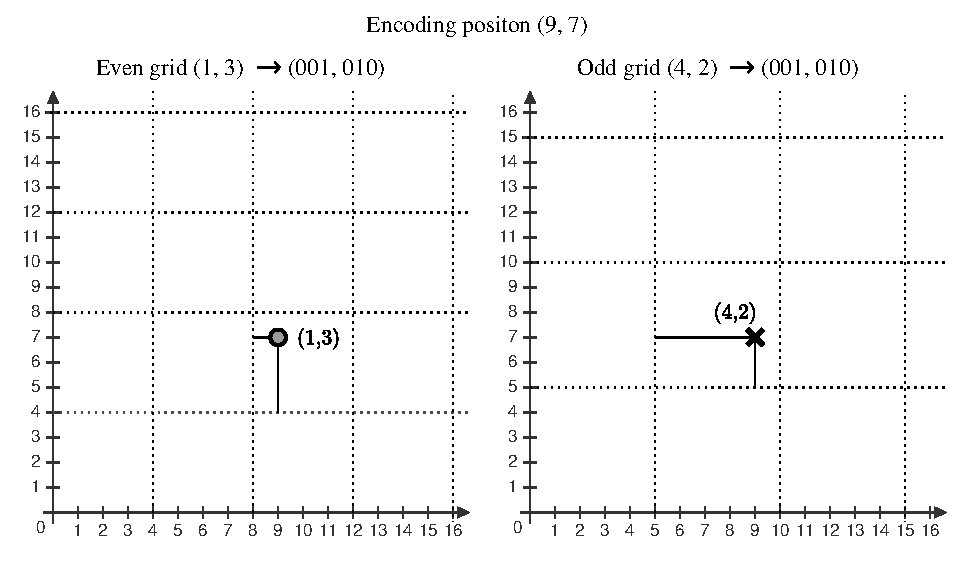
\includegraphics[width=0.9\linewidth]{figures/adsb/cpr_simple_1.pdf}
  \caption{Simplified CPR position coding (encoding)}
  \label{fig:cpr_simple_1}
\end{figure}

With these two grids, we can encode the local positions within each grid systems, which are $(1,3)$ and $(4,2)$, respectively. Now, the position can be encoded only using three bits. 

When the odd and even messages are received, each message alone has different possible global positions, which are shown in Figure \ref{fig:cpr_simple_2}.

\begin{figure}[!ht]
  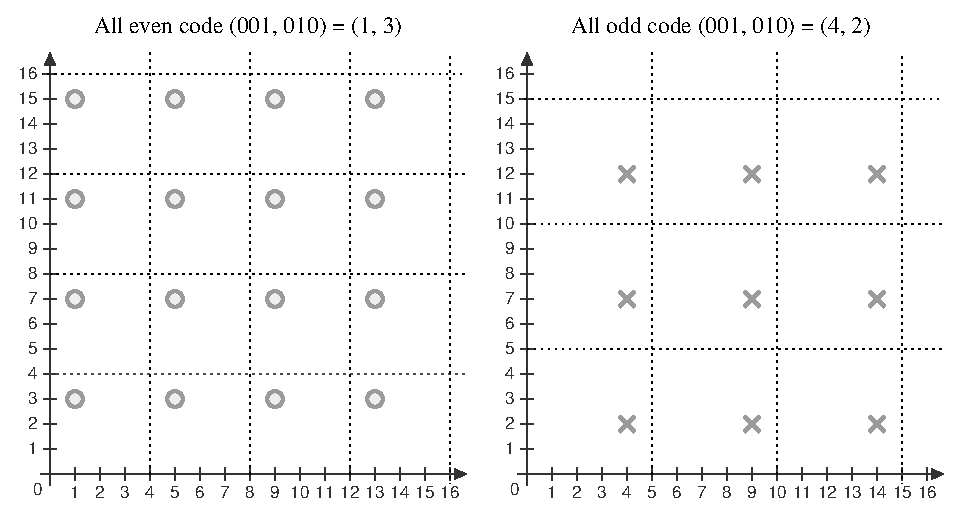
\includegraphics[width=0.9\linewidth]{figures/adsb/cpr_simple_2.pdf}
  \caption{Simplified CPR position coding (all position possiilities)}
  \label{fig:cpr_simple_2}
\end{figure}

Combining the possible positions from both even and odd messages, we can recover the global position where the solutions from both grids overlap with each other. This is shown in Figure \ref{fig:cpr_simple_3}.

\begin{figure}[!ht]
  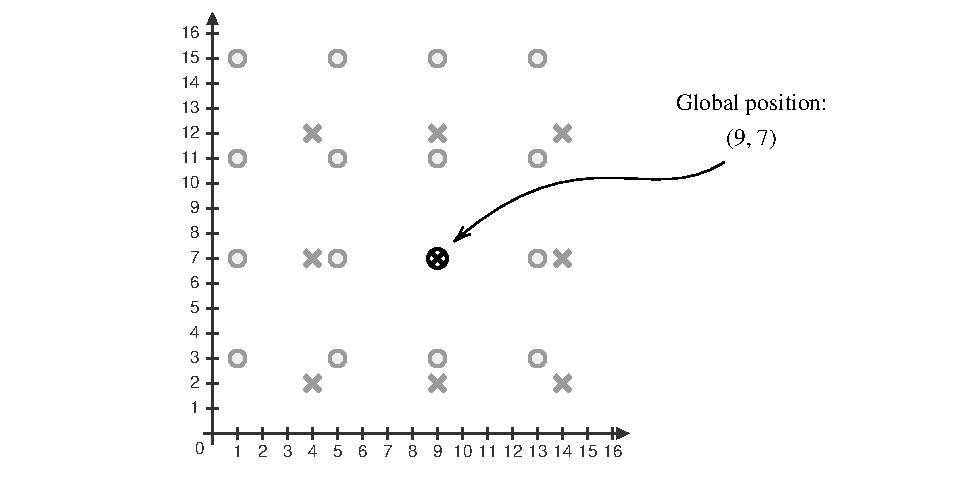
\includegraphics[width=0.9\linewidth]{figures/adsb/cpr_simple_3.pdf}
  \caption{Simplified CPR position coding (final global position)}
  \label{fig:cpr_simple_3}
\end{figure}

\newpage

\section{Compact position reporting}

\subsection{CPR zones}
The actual CPR algorithm is more sophisticated. First of all, more zones are defined. There are 15 latitude zones defined for each hemisphere. Up to 59 longitude zones are used, and the number of longitude zones is different at different altitudes.

Figure \ref{fig:cpr_lat_zones} illustrates the latitude zones. The solid and dashed lines represent the latitude zone size of even and odd messages.

\begin{figure}
  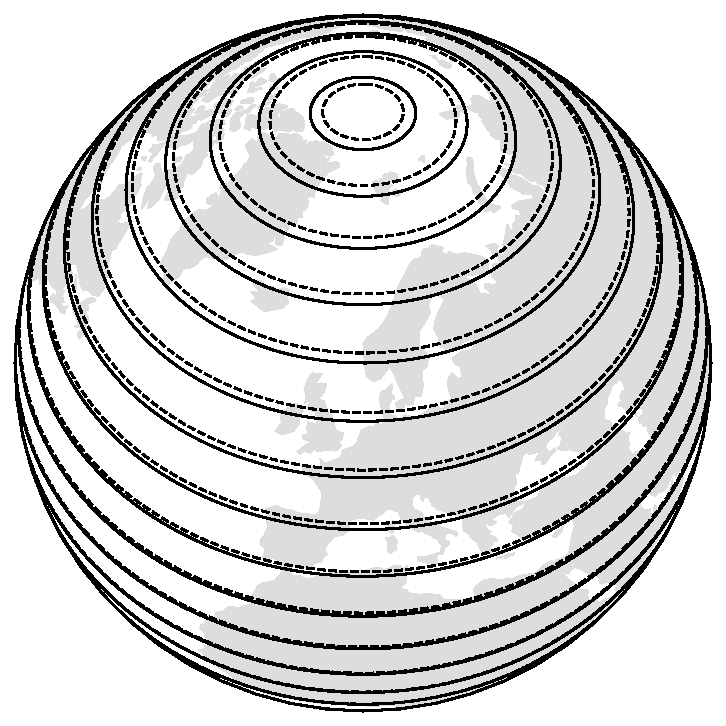
\includegraphics[width=0.7\linewidth]{figures/adsb/cpr_lat_zone_high.pdf} 
  \\
  \vspace{0.5cm}
  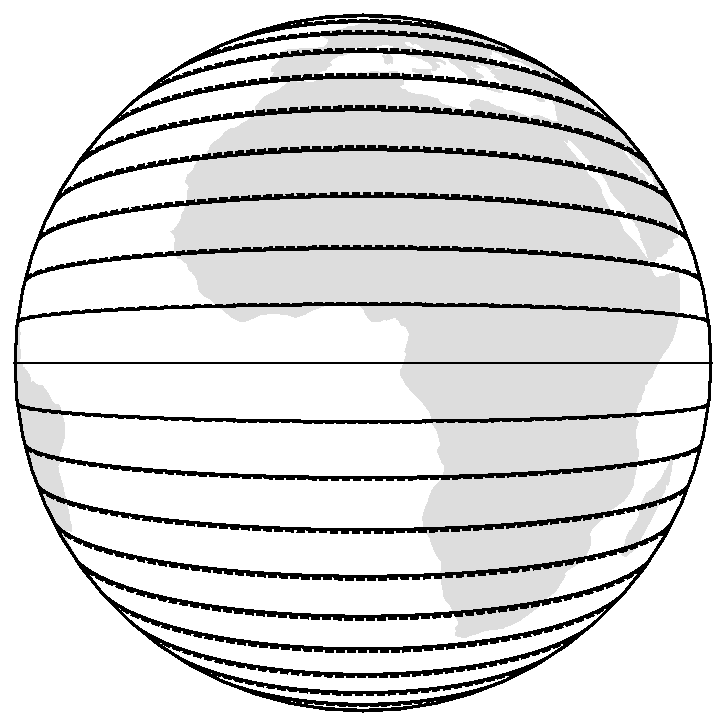
\includegraphics[width=0.7\linewidth]{figures/adsb/cpr_lat_zone_low.pdf}
  \caption{Latitude zones in compact position reporting, from different view points.}
  \label{fig:cpr_lat_zones}
\end{figure}

Figure \ref{fig:cpr_lon_zones} illustrates the latitude zones. The second plot of the figure is a zoomed-in view of the grid of northern Europe. The black and gray lines represent the longitude zone size of even and odd messages respectively. We can see that the number of longitude zones (and the sizes) also differs depending on the latitude.

\begin{figure}
  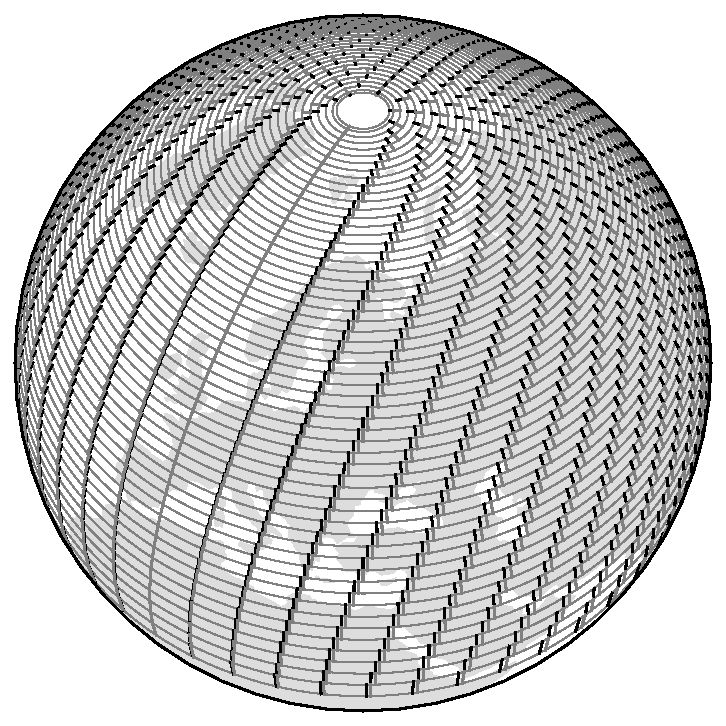
\includegraphics[width=0.7\linewidth]{figures/adsb/cpr_lon_zone_full.pdf}
  \\
  \vspace{0.5cm}
  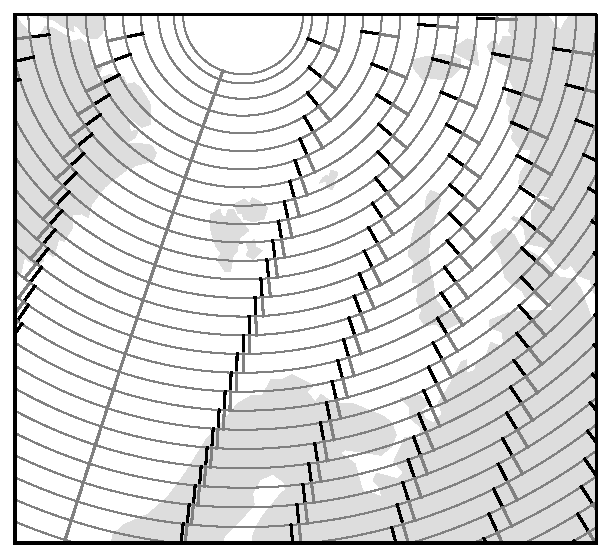
\includegraphics[width=0.7\linewidth]{figures/adsb/cpr_lon_zone_zoom.pdf}
  \caption{Longitude zones in position reporting}
  \label{fig:cpr_lon_zones}
\end{figure}

To report a position, the fractions of latitude and longitude in the respective zones are encoded using 17 bits. These bits are transmitted in the position messages.


\subsection{Core functions and parameters}
To decode the CPR positions, we first introduce relevant parameters and common functions.

\subsubsection{Nz}

$N_Z$ represents the number of latitude zones between the equator and a pole. In Mode~S, $N_Z$ is defined to be 15.

\subsubsection{floor(x)}

The floor function $floor(x)$ returns the greatest integer value $k$, where $k \le x$. For example:

\begin{equation}
  \begin{split}
    floor(5.6) &= 5 \\
    floor(-5.6) &= -6
  \end{split}
\end{equation}

\subsubsection{mod(x, y)}

The modulo function is defined as:

\begin{equation}
  mod(x,y) = x - y \cdot floor \left( \frac{x}{y} \right), \qquad y \ne 0
\end{equation}

\subsubsection{NL(lat) - Longitude zone number}

Given the latitude, this function yields the number of longitude zones between 1 and 59. The function is expressed as:

\begin{equation}
  \mathrm{NL}(\mathrm{lat}) = floor \left\{ \dfrac{2 \pi}{\arccos \left[ 1 - \dfrac{1-\cos \left( \dfrac{\pi}{2~N_Z} \right)}{\cos^2\left(\dfrac{\pi}{180} \cdot \mathrm{lat} \right)} \right] } \right\}
\end{equation}

For latitudes that are close to the equator or the poles, one of following values is returned:

\begin{verbatim}
lat = 0     ->    NL = 59
lat = +87   ->    NL = 2
lat = -87   ->    NL = 2
lat > +87   ->    NL = 1
lat < -87   ->    NL = 1
\end{verbatim}


\section{Globally unambiguous position decoding} 

\subsection{Calculation of latitude} \label{sec:cpr_airborne_global_lat}

In each position message, bit 54 determines whether it is an odd or even type. \0 indicates an even message, while \1 indicates an odd message.

Bits 55--71 and bits 72--88 represent the fractions of the latitude and longitude within the latitude and longitude grid, denoted as $\mathrm{lat}_\mathrm{cpr}$ and $\mathrm{lon}_\mathrm{cpr}$:

\begin{equation}
  \begin{split}
      \mathrm{lat}_\mathrm{cpr} &= \frac{N_{cpr,lat}}{2^{17}} \\
    \mathrm{lon}_\mathrm{cpr} &= \frac{N_{cpr,lon}}{2^{17}}
  \end{split}
\end{equation}


For even and odd messages, the latitude zone sizes are defined as follows:

\begin{equation}
\begin{split}
  \mathrm{dLat}_\mathrm{even} &= \frac{360^\circ}{4 N_Z} \\
  \mathrm{dLat}_\mathrm{odd} &= \frac{360^\circ}{4 N_Z - 1}
\end{split}
\end{equation}


To decode the latitude, first, use the following equation to calculate the latitude zone index, denoted as $j$:

\begin{equation}
  j = floor \left( 59 \cdot \mathrm{lat}_\mathrm{cpr, even} - 60 \cdot \mathrm{lat}_\mathrm{cpr,odd} + \frac{1}{2}  \right)
\end{equation}


Based on both even and odd frames, two latitudes are computed as follows:

\begin{equation}
  \begin{split}
    \mathrm{lat}_\mathrm{even} &= \mathrm{dLat}_\mathrm{even} \Big( mod(j, 60) + \mathrm{lat}_\mathrm{cpr, even} \Big) \\
    \mathrm{lat}_\mathrm{odd} &= \mathrm{dLat}_\mathrm{odd} \Big( mod(j, 59) + \mathrm{lat}_\mathrm{cpr,odd} \Big)
  \end{split}
\end{equation}


For the southern hemisphere, values returned from previous equations range from 270 to 360 degrees. Hence, we need to make sure the latitude is within the range of $[-90, +90]$ by applying the following equations:

\begin{equation}
  \begin{split}
    \mathrm{lat}_\mathrm{even} = \mathrm{lat}_\mathrm{even} - 360,  \quad &\text{if}~\mathrm{lat}_\mathrm{even} \ge 270 \\
    \mathrm{lat}_\mathrm{odd} = \mathrm{lat}_\mathrm{odd} - 360,  \quad &\text{if}~\mathrm{lat}_\mathrm{odd} \ge 270
  \end{split}
\end{equation}


Before proceeding to the longitude calculation, we need to compute $\mathrm{NL}(\mathrm{lat}_\mathrm{even})$ and $\mathrm{NL}(\mathrm{lat}_\mathrm{odd})$ to check if both values are the same. If not, this means the pair of messages are from different longitude zones, and it is not possible to compute the correct global position.

In this case, decoding should be stopped, and it is necessary to wait for a pair of messages that are from the same latitude zone. This situation happens when aircraft are flying across the boundaries of longitude zones.


The final latitude is chosen according to the time stamps of the messages as:

\begin{equation}
  \mathrm{lat} =
  \begin{cases}
   \mathrm{lat}_\mathrm{even}     & \text{if}~T_\mathrm{even} \ge T_\mathrm{odd} \\
   \mathrm{lat}_\mathrm{odd}     & \text{otherwise}
  \end{cases}
\end{equation}

where the current latitude is the more recent of these two latitudes.

\subsection{Calculation of longitude} \label{sec:cpr_airborne_global_lon}

First, the longitude index, $m$, can be calculated as:

\begin{equation}
  m = floor \left( \mathrm{lon}_\mathrm{cpr, even} \cdot \Big[ \mathrm{NL}(\mathrm{lat})-1 \Big] - \mathrm{lon}_\mathrm{cpr,odd} \cdot \mathrm{NL}(\mathrm{lat}) + \frac{1}{2}  \right)
\end{equation}


We also need to calculate the longitude zone size, which is dependent on the latitude. For even and odd messages, the number of longitude zones is defined as:

\begin{equation}
\begin{split}
  n_\mathrm{even} &= max[\mathrm{NL}(\mathrm{lat}), 1] \\
  n_\mathrm{odd} &= max[\mathrm{NL}(\mathrm{lat}-1), 1]
\end{split}
\end{equation}


The longitude zone sizes are defined as follows:

\begin{equation}
\begin{split}
  \mathrm{dLon}_\mathrm{even} &= \frac{360^\circ}{n_\mathrm{even}} \\
  \mathrm{dLon}_\mathrm{odd} &= \frac{360^\circ}{n_\mathrm{odd}}
\end{split}
\end{equation}


Then, the longitude is calculated as:

\begin{equation}
\begin{split}
  \mathrm{lon}_\mathrm{even} &= \mathrm{dLon}_\mathrm{even} \Big[ mod(m, n_\mathrm{even}) + \mathrm{lon}_\mathrm{cpr,even} \Big] \\
  \mathrm{lon}_\mathrm{odd} &= \mathrm{dLon}_\mathrm{odd} \Big[ mod(m, n_\mathrm{odd}) + \mathrm{lon}_\mathrm{cpr,odd} \Big]
  \end{split}
\end{equation}


Similarly, the final longitude is chosen according to the timestamps of the messages as:

\begin{equation}
  \mathrm{lon} =
  \begin{cases}
   \mathrm{lon}_\mathrm{even}     & \text{if}~T_\mathrm{even} \ge T_\mathrm{odd} \\
   \mathrm{lon}_\mathrm{odd}     & \text{otherwise}
  \end{cases}
\end{equation}


It is worth noting that the longitudes in position messages are between 0 and 360 degrees. We often need to convert them to the range between -180 and 180 degrees, which is consistent with aviation conventions. We can convert them as:

\begin{equation}
  \mathrm{lon} = \mathrm{lon} - 360,  \quad \text{if}~\mathrm{lon} \ge 180.
\end{equation}

\subsection{Decoding example}

The example contains two position messages that are received within 10 seconds. The first message is the most recent position message transmitted by the aircraft.

\begin{verbatim}
8D40621D58C382D690C8AC2863A7   (most recent)
8D40621D58C386435CC412692AD6
\end{verbatim}

Following the common ADS-B message structure, we can identify the ICAO address and ME field as follows:

\begin{verbatim}
+----+--------+----------------+--------+
|    | ICAO   |       ME       |  PI    |
+----+--------+----------------+--------+
| 8D | 40621D | 58C382D690C8AC | 2863A7 |
| 8D | 40621D | 58C386435CC412 | 692AD6 |
+----+--------+----------------+--------+
\end{verbatim}

We can covert the message data into binary format:

\begin{verbatim}
+-------+-----+--------------+---+---+-------------------+-------------------+
| TC    |     | ALT          | T | F | CPR-LAT           | CPR-LON           |
+-------+-----+--------------+---+---+-------------------+-------------------+
| 01011 | 000 | 110000111000 | 0 | 0 | 10110101101001000 | 01100100010101100 |
| 01011 | 000 | 110000111000 | 0 | 1 | 10010000110101110 | 01100010000010010 |
+-------+-----+--------------+---+---+-------------------+-------------------+
\end{verbatim}

It is possible to extract the encoded CPR latitude and longitude binary and convert them to decimal format. Then, these values are divided by the $2^{17}$, representing the fractions of the positions within the latitude and longitude grids:

\begin{equation}
  \begin{split}
    \mathrm{lat}_\mathrm{cpr,even} &= \frac{93000}{2^{17}} \\
    \mathrm{lon}_\mathrm{cpr,even} &= \frac{51372}{2^{17}} \\
    \mathrm{lat}_\mathrm{cpr,odd} &=  \frac{74158}{2^{17}} \\
    \mathrm{lon}_\mathrm{cpr,odd} &=  \frac{50194}{2^{17}}
  \end{split}
\end{equation}

We can calculate the latitude index, $j$, as:

\begin{equation}
  j = floor \left( 59 \times \frac{93000}{2^{17}} - 60 \times \frac{51372}{2^{17}} + \frac{1}{2}  \right) = 8
\end{equation}

Then, we can decode the latitudes from both even and odd messages:

\begin{equation}
  \begin{split}
    \mathrm{lat}_\mathrm{even} &= \frac{360}{4 \times 15} \Big[ mod(8, 60) + \frac{93000}{2^{17}} \Big] = 52.25720214843750 \\
    \mathrm{lat}_\mathrm{odd} &= \frac{360}{4 \times 15 - 1} \Big[ mod(8, 59) + \frac{74158}{2^{17}} \Big] = 52.26578017412606
  \end{split}
\end{equation}

After validating the longitude zone of both messages:

\begin{equation}
  \begin{split}
    \mathrm{NL}(\mathrm{lat}_\mathrm{even}) &= \mathrm{NL}(52.25720214843750) = 36 \\
    \mathrm{NL}(\mathrm{lat}_\mathrm{odd}) &= \mathrm{NL}(52.26578017412606) = 36
  \end{split}
\end{equation}

we can continue to calculate the global position. Since the even message is the most recent message, the latitude is:

\begin{equation}
  \mathrm{lat} = \mathrm{lat}_\mathrm{even} = 52.25720214843750
\end{equation}

The final longitude (based on the even message) is calculated as:

\begin{align}
  m &= floor \left( \frac{51372}{2^{17}} \times (36-1) - \frac{50194}{2^{17}} \times 36 + \frac{1}{2}  \right) = 0\\
  n &= max \Big( 36-0, 1 \Big) = 36\\
    \mathrm{lon} &= \frac{360}{36} \Big[ mod(0, 36) + \frac{51372}{2^{17}} \Big] = 3.91937255859375
\end{align}

\begin{notebox}{Try it out}
Using pyModeS, we can perform the previous calculation of globally unambiguous position as: 

\begin{verbatim}
import pyModeS as pms

msg0 = "8D40621D58C382D690C8AC2863A7"
msg1 = "8D40621D58C386435CC412692AD6"
t0 = 1457996402
t1 = 1457996400

pms.adsb.position(msg0, msg1, t0, t1)
\end{verbatim}

Output: 

\begin{verbatim}
(52.2572, 3.91937)
\end{verbatim}

\end{notebox}



\section{Locally unambiguous position decoding}

Previously, a globally unambiguous position was decoded using a pair of odd and even messages. In this part, we will discuss how to decode the ADS-B position with one message and a previous reference position that is obtained using globally unambiguous decoding.

This method offers the possibility to continuous decode aircraft using only one message. It computes the latitude index (j) and the longitude index (m) based on this existing reference position and can be applied to both odd and even messages.

\subsection{The reference position}

The reference position should be close to the actual position, which must be within a 180 NM range. For example, this can be the position of the aircraft that has been decoded in the previous update. The range limitation is to ensure the consistency of the latitude and longitude zones between the reference position and the decoding position. The reference position is denoted as ($\mathrm{lat}_\mathrm{ref}$, $\mathrm{lon}_\mathrm{ref}$).

\subsection{Calculation of latitude}

Denote $i$ as the value dependent on the type of the message:

\begin{equation}
  i =
  \begin{cases}
    0, \quad \text{even message} \\
    1, \quad \text{odd message}
  \end{cases}
\end{equation}

\noindent The latitude zone size is different depending on the message type:

\begin{equation}
  \mathrm{dLat} = \frac{360}{4n_z-i}
\end{equation}

Then, the latitude zone index, $j$, is calculated as:

\begin{equation}
  j = floor \left( \frac{\mathrm{lat}_\mathrm{ref}}{\mathrm{dLat}} \right) + floor \left[ \frac{mod(\mathrm{lat}_\mathrm{ref}, \mathrm{dLat})}{\mathrm{dLat}}  - \mathrm{lat}_\mathrm{cpr}  + \frac{1}{2} \right]
\end{equation}

Knowing the latitude zone index, the latitude of the new position is:

\begin{equation}
  \mathrm{lat} = \mathrm{dLat} \cdot (j + \mathrm{lat}_\mathrm{cpr})
\end{equation}


\subsection{Calculation of longitude}

Next, we can calculate the increment of the longitude per zone based on the decoded latitude, which is dependent on both message type and latitude:

\begin{equation}
  \mathrm{dLon} = \frac{360}{max\Big( \mathrm{NL}(\mathrm{lat})-i, 1 \Big)}
\end{equation}


Then, the longitude zone index, $m$, is calculated as:

\begin{equation}
  m = floor \left( \frac{\mathrm{lon}_\mathrm{ref}}{\mathrm{dLon}} \right) + floor \left( \frac{mod(\mathrm{lon}_\mathrm{ref}, \mathrm{dLon})}{\mathrm{dLon}}  - \mathrm{lon}_\mathrm{cpr}  + \frac{1}{2}  \right)
\end{equation}

Knowing the longitude zone index, the longitude of the new position is:

\begin{equation}
  \mathrm{lon} = \mathrm{dLon} \cdot (m + \mathrm{lon}_\mathrm{cpr})
\end{equation}


\subsection{Decoding example}

Next, we illustrate the decoding process of the messages from the previous example with a reference position. The message and the reference position are as follows:

\begin{verbatim}
Message:   8D40621D58C382D690C8AC2863A7
ME (data):         58C382D690C8AC

Reference position: (52.258, 3.918)
\end{verbatim}

We can easily convert the message data to binary format as:

\begin{verbatim}
+-------+-----+--------------+-----------------------------------------------+
| TC    |     | ALT          | T | F | CPR-LAT           | CPR-LON           |
|-------+-----+--------------+---+---+-------------------+-------------------|
| 01011 | 000 | 110000111000 | 0 | 0 | 10110101101001000 | 01100100010101100 |
+-------+-----+--------------+---+---+-------------------+-------------------+
|       |     |              |   |   | 93000             | 51372             |
+-------+-----+--------------+---+---+-------------------+-------------------+
\end{verbatim}

First, since this is an even message ($i=0$), we can calculate the latitude as follows:

\begin{align}
  \mathrm{dLat} &= \frac{360}{4 \times 15 - 0} = 6 \\
  j &= floor \left( \frac{52.258}{6} \right) + floor \left[ \frac{mod(52.258, 6)}{6} - \frac{93000}{2^{17}}  + \frac{1}{2} \right] = 8 \\
  \mathrm{lat} &= 6 \times \left( 8 + \frac{93000}{2^{17}} \right) = 52.2572021484375
\end{align}

Next, the longitude can be calculated as follows:

\begin{align}
  \mathrm{dLon} &= \frac{360}{max \Big( \mathrm{NL}(\mathrm{lat}_\mathrm{even})-0, 1 \Big)} = \frac{360}{max(36, 1)} = 10 \\
  m &= floor \left( \frac{3.918}{10} \right) + floor \left( \frac{mod(3.918, 10)}{10} - \frac{51372}{2^{17}}  + \frac{1}{2}  \right) = 0 \\
  \mathrm{lon} &= 10 \times \left(0 + \frac{51372}{2^{17}} \right) = 3.91937255859375
\end{align}

%
% d_lat:  6
% j:      8
% lat:    52.25720
% m:      0
% d_lon:  10
% lon:    3.91937

\begin{notebox}{Try it out}
Using pyModeS, we can perform the previous locally unambiguous position calculation as: 

\begin{verbatim}
import pyModeS as pms

msg = "8D40621D58C382D690C8AC2863A7"
lat_ref = 52.258
lon_ref = 3.918

pms.adsb.position_with_ref(msg, lat_ref, lon_ref)
\end{verbatim}

Output: 

\begin{verbatim}
(52.2572, 3.91937)
\end{verbatim}

\end{notebox}


\section{Altitude decoding}

The altitude of the aircraft can be decoded with one position message, regardless of it being an even or odd type. However, depending on the type code of the messages, the altitudes are decoded differently. Table \ref{tb:adsb-tc} from Chapter \ref{chap:adsb-basic} shows two different types of altitudes. They are:

\begin{itemize}
\item \textbf{TC=9--18}: Airborne position, with barometric altitude encoded (in feet)
\item \textbf{TC=20--22}: Airborne position, with GNSS Height encoded (in meters)
\end{itemize}

\subsection{Barometric altitude}
For barometric altitude (TC between 9 and 18), the 8th bit of the 12-bit altitude field is the \emph{Q bit}. It indicates whether the altitude is encoded with an increment of 25 feet or 100 feet.

When $Q=1$, the altitude is encoded with a 25 feet increment. Removing the Q-bit, the altitude shall be the multiple of 25 feet minus 1000 feet:

\begin{equation}
  h = 25 ~ N - 1000 \quad \text{(ft)}
\end{equation}

For example, based the example message in the previous section, the 12 bits in the altitude field can be read as follows:

\begin{verbatim}
1100001 1 1000
        ^
       Q-bit
\end{verbatim}

Once the Q-bit is removed, the decimal representation of the remaining bits is 1560:

\begin{verbatim}
11000011000 -> 1560
\end{verbatim}

The altitude of the aircraft becomes:

\begin{equation}
1560 \times 25 - 1000 = 38000 \quad \text{(ft)}
\end{equation}

In the case where the altitude is higher than 50175 feet, a 100 feet increment is used. In this situation, the Q bit is set to \0, and the rest of the bits are encoded using Gray code \cite{doran2007}. It is worth noting that it is possible for all altitude bits to be zeros,which indicates that the altitude information is not available.


\subsection{GNSS height}

When the position message has the Type Code from 20 to 22, the 12-bit altitude field is used for the encoding of the GNSS height. The GNSS height is derived from the global positioning satellites, and the decimal value of all 12 bits translates into the height of aircraft in meters.

\begin{notebox}{Try it out}
Using pyModeS, we can perform the altitude decoding as: 

\begin{verbatim}
import pyModeS as pms

msg = "8D40621D58C382D690C8AC2863A7"

pms.adsb.altitude(msg)
\end{verbatim}

Output (altitude in feet): 

\begin{verbatim}
38000
\end{verbatim}
\end{notebox}



\section{Verification of decoded positions}

It is recommended to perform a so-called \emph{reasonable test} to validate the decoded position. There are a couple of ways to perform such test to examine the plausibility of decoded positions:

\begin{enumerate}
  \item The first approach is to use the receiver position. The decoded position should not exceed the coverage of the receiver. See Chapter \ref{chap:quickstart}, Figure \ref{fig:max_range_curve}.

  \item A further test is to use more than one pair of different messages to produce multiple globally unambiguous positions. Then, the distance between these positions can be used to examine whether the decoded positions are reasonable.
\end{enumerate}

If the decoded position fails the reasonable tests, it should be discarded.

\chapter{Surface position}

When an aircraft is on the ground, a different type of message is used to broadcast its position information. Unlike the airborne position message, the surface position message also includes the speed of the aircraft. Since no altitude information needs to be transmitted, this provides extra bits for extra information, such as speed and track angle.

The surface position message has the Type Code from 5 to 8, which also represents the level of uncertainties in the position. And the structure of the surface position message payload is shown as follows:


\begin{verbatim}
+-------+--------+------+--------+------+------+-------------+-------------+
| TC, 5 | MOV, 7 | S, 1 | TRK, 7 | T, 1 | F, 1 | LAT-CPR, 17 | LON-CPR, 17 |
+-------+--------+------+--------+------+------+-------------+-------------+
\end{verbatim}

We can see that the fields are defined similarly to the ones from airborne messages, except that the surveillance status and altitude bits are replaced by movement and ground track. The details of the fields are shown in Table \ref{tb:adsb-surf-pos-fields}

\begin{table}[ht]
\caption{Surface position message structure}
\label{tb:adsb-surf-pos-fields}
\begin{tabular}{|l|l|l|l|l|}
\hline
\textbf{FIELD} & \textbf{} & \textbf{MSG} & \textbf{MB} & \textbf{BITS} \\ \hline
Type Code & TC & 33-37 & 1-5 & 5 \\ \hline
Movement & MOV & 38-44 & 6-12 & 7 \\ \hline
Status for ground track & S & 45 & 13 & 1\\
~~0: Invalid & & & &\\
~~1: Valid & & & &\\ \hline
Ground track & TRK & 46-52 & 14-20 & 7 \\ \hline
Time & T & 53 & 21 & 1 \\ \hline
CPR Format  & F & 54 & 22 & 1\\
~~0: even frame & & & &\\
~~1: odd frame & & & &\\ \hline
Encoded latitude & LAR-CPR & 55-71 & 23-39 & 17 \\ \hline
Encoded longitude & LON-CPR & 72-88 & 40-56 & 17 \\ \hline
\end{tabular}
\end{table}

\section{Movement}

The movement field encodes the aircraft ground speed. The ground speed of the aircraft is encoded non-linearly and with different quantizations. This is to ensure that a lower speed can be encoded with a improved precision than a higher speed. Different levels of quantizations are defined in Table \ref{tb:adsb-surf-pos-mov}.

\begin{table}[ht]
\caption{Surface position movement (ground speed) decoding}
\label{tb:adsb-surf-pos-mov}
\begin{tabular}{|l|l|l|}
\hline
\textbf{Encoded speed} & \textbf{Ground speed range} & \textbf{Quantization} \\ \hline
0 & Speed not available &  \\ \hline
1 & Stopped (v $<$ 0.125 kt) &  \\ \hline
2 - 8 & 0.125 $\leq$ v $<$ 1 kt & 0.125 kt steps \\ \hline
9 - 12 & 1 kt $\leq$ v $<$ 2 kt & 0.25 kt steps \\ \hline
13 - 38 & 2 kt $\leq$ v $<$ 15 kt & 0.5 kt steps \\ \hline
39 - 93 & 15 kt $\leq$ v $<$ 70 kt & 1 kt steps \\ \hline
94 - 108 & 70 kt $\leq$ v $<$ 100 kt & 2 kt steps \\ \hline
109 - 123 & 100 kt $\leq$ v $<$ 175 kt & 5 kt steps \\ \hline
124 & v $\ge$ 175 kt &  \\ \hline
125 - 127 & Reserved &  \\ \hline
\end{tabular}
\end{table}


\section{Ground track}

The ground track is encoded with a precision of (and rounded to) 360/128 degrees. Zero degrees represents an aircraft ground track that is aligned with the true north. Based on the encoded value ($n$), the ground track ($\chi$) is calculated as:

\begin{equation}
    \chi = \frac{360~n}{128} \quad \text{(degrees)}
\end{equation}

When the status for the ground track field is set to 0, the information contained in the ground track fields should be considered as invalid.

\section{Position}

Like coordinates from airborne messages, the surface latitude and longitude are also encoded in the Compact Position Reporting (CPR) format. CPR format bit indicates whether the message is a \emph{even} or \emph{odd} message. There are only a few slight differences in decoding the surface position positions. 

First, the latitude zone size is four times smaller, which is defined as:

\begin{equation}
\begin{split}
    \mathrm{dLat}_\mathrm{even} &= \frac{90^\circ}{4 N_Z} \\
    \mathrm{dLat}_\mathrm{odd} &= \frac{90^\circ}{4 N_Z - 1}
\end{split}
\end{equation}

Similarly, the longitude zone size is also smaller, which is:

\begin{equation}
\begin{split}
    \mathrm{dLon}_\mathrm{even} &= \frac{90^\circ}{n_\mathrm{even}} \\
    \mathrm{dLon}_\mathrm{odd} &= \frac{90^\circ}{n_\mathrm{odd}}
\end{split}
\end{equation}

The algorithm used to encode the position is essentially the same as the one used for encoding airborne position. All the other equations from chapter \ref{chap:airborn-position} can be used to decode surface position.

The main difference, when compared to the airborne position, is that the original number of bits used for encoding surface coordinates is 19 instead of 17. However in the message, only the lower-order 17 bits are included and transmitted in the surface message. Thus, there can be multiple solutions for a pair of odd and even messages, even when globally unambiguous decoding is used. To identify the correct solution, a reference position needs to be given. This can be the position of the receiver or the location of the airfield.

When employing locally unambiguous decoding, the reference position needs to be within 45 nautical miles of the actual location. Commonly, the positions of the airport is used.

With the equations from section \ref{sec:cpr_airborne_global_lat}, the solution refers to the latitude located at the northern hemisphere. We need to compute a southern hemisphere solution by subtracting this value with 90 degrees. The final correct latitude is the one that is closet to the reference position.

Similarly, with the equations from section \ref{sec:cpr_airborne_global_lon}, the solution refers only the longitude in the 0 to 90 degrees quadrant. We need to compute the other three possible solutions by adding 90, 180, and 270 degrees. The final correct longitude is also the one that is closet to the reference position.




\section{Example}

\subsection{Globally unambiguous decoding}

First, we decode the location using globally unambiguous decoding. The following example contains an even/odd pair of surface position messages: 

\begin{verbatim}
8C4841753AAB238733C8CD4020B1
8C4841753A8A35323FAEBDAC702D    (most recent)
\end{verbatim}

Based on the ADS-B message structure, we can identify the ICAO address and message payload data as follows:

\begin{verbatim}
+----+--------+----------------+--------+
|    | ICAO   |      Data      |  PI    |
+----+--------+----------------+--------+
| 8C | 484175 | 3AAB238733C8CD | 4020B1 |
| 8C | 484175 | 3A8A35323FAEBD | AC702D |
+----+--------+----------------+--------+
\end{verbatim}

We can covert the message data into binary format:

\begin{verbatim}
+-------+---------+---+---------+---+---+-------------------+-------------------+
| TC    | MOV     | S | TRK     | T | F | CPR-LAT           | CPR-LON           |
+-------+---------+-------------+---+---+-------------------+-------------------+
| 00111 | 0101010 | 1 | 0110010 | 0 | 0 | 11100001110011001 | 11100100011001101 |
| 00111 | 0101000 | 1 | 0100011 | 0 | 1 | 01001100100011111 | 11010111010111101 |
+-------+---------+---+---------+---+---+-------------------+-------------------+
\end{verbatim}


Knowing the receiver location:

\begin{verbatim}
reference latitude: 51.990
reference longitude: 4.375
\end{verbatim}


it is possible to extract the encoded CPR latitude and longitude binary and convert them to decimal format. Then, they are divided by the $2^{17}$, representing the fractions of the positions within the latitude and longitude grids:

\begin{equation}
  \begin{split}
    \mathrm{lat}_\mathrm{cpr,even} &= \frac{115609}{2^{17}} \\
    \mathrm{lon}_\mathrm{cpr,even} &= \frac{116941}{2^{17}} \\
    \mathrm{lat}_\mathrm{cpr,odd} &=  \frac{39199}{2^{17}} \\
    \mathrm{lon}_\mathrm{cpr,odd} &=  \frac{110269}{2^{17}}
  \end{split}
\end{equation}

We can calculate the latitude index, $j$, as:

\begin{equation}
  j = floor \left( 59 \times \frac{115609}{2^{17}} - 60 \times \frac{39199}{2^{17}} + \frac{1}{2}  \right) = 34
\end{equation}

Then, we can decode the latitudes from both even and odd messages:

\begin{equation}
  \begin{split}
    \mathrm{lat}_\mathrm{even} &= \frac{90}{4 \times 15} \Big[ mod(34, 60) + \frac{115609}{2^{17}} \Big] = 52.323040008544920 \\
    \mathrm{lat}_\mathrm{odd} &= \frac{90}{4 \times 15 - 1} \Big[ mod(34, 59) + \frac{39199}{2^{17}} \Big] = 52.320607072215964
  \end{split}
\end{equation}

After validating the longitude zone of both messages are the same:

\begin{equation}
  \begin{split}
    \mathrm{NL}(\mathrm{lat}_\mathrm{even}) &= \mathrm{NL}(52.323040008544920) = 36 \\
    \mathrm{NL}(\mathrm{lat}_\mathrm{odd}) &= \mathrm{NL}(52.320607072215964) = 36
  \end{split}
\end{equation}


we can continue to calculate the global position. Since the even message is the most recent message, the northern hemisphere latitude solution is:

\begin{equation}
  \mathrm{lat}_N = \mathrm{lat}_\mathrm{odd} = 52.320607072215964
\end{equation}


The southern hemisphere latitude solution is:

\begin{equation}
    \mathrm{lat}_S = 52.320607072215964 - 90 = -37.679392927784036
\end{equation}
  
By comparing the result with the reference latitude (51.990), the final latitude value is the one located in the northern hemisphere.

\begin{equation}
    \mathrm{lat} = \mathrm{lat}_N = 52.320607072215964
\end{equation}
  

The longitude solution in the first quadrant of 0 to 90 degress is calculated based on the most recent (odd) message:

\begin{align}
  m &= floor \left( \frac{116941}{2^{17}} \times (36-1) - \frac{110269}{2^{17}} \times 36 + \frac{1}{2}  \right) = 1\\
  n &= max \Big( 36-1, 1 \Big) = 35\\
    \mathrm{lon}_1 &= \frac{90}{35} \Big[ mod(1, 36-1) + \frac{110269}{2^{17}} \Big] = 4.734734671456474
\end{align}

The three other possible solutions are:

\begin{equation}
\begin{split}
    \mathrm{lon}_2 &= \mathrm{lon}_1 + 90 = 94.734734671456474 \\
    \mathrm{lon}_3 &= \mathrm{lon}_1 + 180 = 184.734734671456474 \\
    \mathrm{lon}_4 &= \mathrm{lon}_1 + 270 = 274.734734671456474 \\
\end{split}
\end{equation}

By comparing with the reference longitude (4.375), the final longitude is the one located in the first quadrant. Combining the result of previously obtained latitude, the final decoded coordinates (rounded up to 6 decimal position) are:


\begin{verbatim}
latitude: 52.320607
longitude: 4.734735
\end{verbatim}

\begin{notebox}{Try it out}
Using \texttt{pyModeS}, we can perform the decoding of this globally unambiguous surface position as: 

\begin{verbatim}
import pyModeS as pms

msg0 = "8C4841753AAB238733C8CD4020B1"
msg1 = "8C4841753A8A35323FAEBDAC702D"
t0 = 1457996410
t1 = 1457996412
lat_ref = 51.990
lon_ref = 4.375

position = pms.adsb.position(msg0, msg1, t0, t1, lat_ref, lon_ref)
\end{verbatim}

Note that the reference coordinates are needed for decoding the surface position. In this case the reference is the coordinates of the airfield. 

\end{notebox}



\subsection{Locally unambiguous decoding}

Secondly, we decode the location using locally unambiguous decoding. In this case, we want to use the position obtained previously as the reference.

The new message received is:

\begin{verbatim}
8C4841753A9A153237AEF0F275BE
\end{verbatim}

The structure of the ADS-B message is:

\begin{verbatim}
+----+--------+----------------+--------+
|    | ICAO   |      Data      |  PI    |
+----+--------+----------------+--------+
| 8C | 484175 | 3A9A153237AEF0 | F275BE |
+----+--------+----------------+--------+
\end{verbatim}

We can covert the message data into binary format:

\begin{verbatim}
+-------+---------+---+---------+---+---+-------------------+-------------------+
| TC    | MOV     | S | TRK     | T | F | CPR-LAT           | CPR-LON           |
+-------+---------+-------------+---+---+-------------------+-------------------+
| 00111 | 0101001 | 1 | 0100001 | 0 | 1 | 01001100100011011 | 11010111011110000 |
+-------+---------+---+---------+---+---+-------------------+-------------------+
\end{verbatim}


\begin{align}
    \mathrm{dLat} &= \frac{90}{4 \times 15 - 1} = \frac{90}{59} \\
    j &= floor \left( \frac{52.320607}{90/59} \right) + floor \left[ \frac{mod(52.320607, 90/59)}{90/59} - \frac{39195}{2^{17}}  + \frac{1}{2} \right] = 34 \\
    \mathrm{lat} &= \mathrm{lat}_\mathrm{odd} = \frac{90}{59} \times \left( 34 + \frac{39195}{2^{17}} \right) = 52.32056051997815
\end{align}
  
Next, the longitude can be calculated as follows:
  
\begin{align}
    \mathrm{dLon} &= \frac{90}{max \Big( \mathrm{NL}(\mathrm{lat}_\mathrm{odd})-1, 1 \Big)} = \frac{90}{max(36-1, 1)} = \frac{90}{35} \\
    m &= floor \left( \frac{4.734735}{90/35} \right) + floor \left( \frac{mod(4.734735, 90/35)}{90/35} - \frac{110320}{2^{17}}  + \frac{1}{2}  \right) = 1 \\
    \mathrm{lon} &= \frac{90}{35} \times \left(1 + \frac{110320}{2^{17}} \right) = 4.735735212053571
\end{align}


The final decoded coordinates (rounded up to 6 decimal positions) are:

\begin{verbatim}
latitude: 52.320561
longitude: 4.735735
\end{verbatim}

\begin{notebox}{Try it out}
Using \texttt{pyModeS}, we can perform the decoding of this locally unambiguous surface position as: 

\begin{verbatim}
import pyModeS as pms

msg = "8C4841753A9A153237AEF0F275BE"
lat_ref = 51.990
lon_ref = 4.375

position = pms.adsb.position_with_ref(msg, lat_ref, lon_ref)
\end{verbatim}

\end{notebox}


\subsection{Movement and track}

As a continuation of the previous example, we can also calculate the speed and track angle from the movement and track fields.

The decimal value of movement \texttt{0101001} is \texttt{41}. Based on Table \ref{tb:adsb-surf-pos-mov}, the speed is encoded using 1 kt steps. Thus, the speed of aircraft is:

\begin{equation}
  15 + (42 - 39) \times 1 = 17 kt
\end{equation}

The decimal value of track angle \texttt{0100001} is \texttt{33}. The track angle can be calculated as:

\begin{equation}
  \frac{360^\circ}{128} \times 33 = 92.8125 ^\circ
\end{equation}

\begin{notebox}{Try it out}
Using \texttt{pyModeS}, we can perform the decoding aircraft speed and track angle as: 

\begin{verbatim}
import pyModeS as pms

msg = "8C4841753A9A153237AEF0F275BE"

spd, trk, vs, tag = pms.adsb.velocity(msg)
\end{verbatim}

Note that the last two parameters returned by the previous function are vertical speed and a tag indicate whether the speed is ground speed (GS) or airspeed (IAS/TAS).

\end{notebox}

\chapter{Airborne velocity}

Airborne velocities are all transmitted with Type Code 19 (\texttt{TC=19}). Four different subtypes are defined with bit 6 to 8 in the message payload bits. With subtypes 1 and 2, ground speeds of aircraft are reported. With subtypes 3 and 4, aircraft true airspeed or indicated airspeed are included. Reporting of airspeed in ADS-B only occurs when aircraft position can not be determined based on the GNSS system.\footnote{In the real world, subtype 3 messages are very rare.}

Among all four different sub-types, sub-type 2 and 4 are designed for supersonic aircraft. Their message structures are identical to subtypes 1 and 3, but with the speed resolution of 4 kt instead of 1 kt. However, since there are no operational supersonic airliners currently, there is no ADS-B airborne velocity message with sub-type 2 and 4.

These messages contain more information than just horizontal and vertical velocity. Two other significant types of information are the navigation uncertainty category for velocity, and the difference between the GNSS height and barometric altitude. For instance, the study in \cite{stone2015} has made use of the later information to better model the air temperature at higher altitudes.

All sub-types share a similar overall message structure, with the different definitions from message bits 14 to 35 (or frame bits 46 to 67). The general structure of the message is shown in Table \ref{tb:adsb-velocity-bits}. 

\begin{table}[]
\caption{Airborne velocity message structure}
\label{tb:adsb-velocity-bits}
\footnotesize
\begin{tabular}{|l|l|c|c|c|}
\hline
\textbf{FIELD} & & \textbf{MSG} & \textbf{ME} & \textbf{BITS} \\ \hline
\hline
\textbf{Type Code} & TC & 33-37 & 1-5 & 5\\
~~TC=19 {[}Binary: 10011{]} &&&& \\ \hline
\textbf{Sub-type} & ST & 38-40 & 6-8 & 3\\
~~1: Subsonic &&&&\\
~~2: Supersonic &&&& \\ \hline
\textbf{Intent change flag} & IC & 41 & 9 & 1 \\ \hline
\textbf{IFR capability flag} & IFR & 42 & 10 & 1 \\ \hline
\textbf{Navigation uncertainty category for velocity} & & 43-45 & 11-13 & 3\\
~~ADS-B version 0 & NUCr &&&\\
~~ADS-B version 1-2 & NUCv &&&\\ \hline
\hline
\textbf{Sub-type specific fields} & & 46-67 & 14-35 & 22\\
~~Refer to Table \ref{tb:adsb-velocity-bits-14-35-gs} and Table \ref{tb:adsb-velocity-bits-14-35-as} &&&& \\ \hline
\hline
\textbf{Source bit for vertical rate} & VrSrc & 38 & 36 & 1 \\
~~0: GNSS, 1: Barometer &&&&\\ \hline
\textbf{Sign bit for vertical rate}  & Svr & 69 & 37 & 1 \\
~~0: Up, 1: Down &&&& \\ \hline
\textbf{Vertical rate} & VR & 70-78 & 38-46 & 9\\
~~All zeros: no information &&&&\\
~~LSB: 64 ft/min &&&&\\
~~VR = 64 x (Decimal value - 1) &&&& \\ \hline
\textbf{Reserved} &  & 79-80 & 47-48 & 2 \\ \hline
\textbf{Sign bit for GNSS and Baro altitudes difference} & SDif & 81 & 49 & 1\\
~~0: GNSS alt above Baro alt &&&& \\
~~1: GNSS alt below Baro alt &&&& \\ \hline
\textbf{Difference between GNSS and Baro altitudes} & dAlt & 82-88 & 50-56 & 7\\
~~All zeros: no information &&&&\\
~~LSB: 25 ft &&&& \\ \hline
\end{tabular}
\end{table}

Comparing to position messages, the decoding of velocity messages is more straight forward since there is no complicated encoding scheme. In this chapter, we are going to explain the decoding process.

\section{Example messages}

Throughout this chapter, we will use two example messages to illustrate the decoding process:

\begin{verbatim}
Message A:  8D485020994409940838175B284F (sub-type 1)
Message B:  8DA05F219B06B6AF189400CBC33F (sub-type 3)
\end{verbatim}

By decomposing the messages, the downlink format, ICAO address, message payload, and CRC remainder are shown as follows:

\begin{verbatim}
Message A (sub-type 1):
+----+--------+----------------+--------+
| DF | ICAO   | ME             |  CRC   |
+----+--------+----------------+--------+
| 8D | 485020 | 99440994083817 | 5B284F |
+----+--------+----------------+--------+
\end{verbatim}

\begin{verbatim}
Message B (sub-type 3):
+----+--------+----------------+--------+
|    | ICAO   | ME             |  CRC   |
+----+--------+----------------+--------+
| 8D | A05F21 | 9B06B6AF189400 | CBC33F |
+----+--------+----------------+--------+
\end{verbatim}

Next, we can convert both message payloads (ME fields) into binary and decompose the structure further as follows:

\begin{verbatim}
Message A (sub-type 1):
+-----+---+--+---+---+-----------+-----+---+---------+----+----+-------+
|TC   |ST |IC|IFR|NUC|           |VrSrc|Svr|VR       |RESV|SDif|DAlt   |
+-----+---+--+---+---+-----------+-----+---+---------+----+----+-------+
|10011|001|0 |1  |000|10000001001|0    |1  |000001110|00  |0   |0010111|
|     |   |  |   |   |10010100000|     |   |         |    |    |       |
+-----+---+--+---+---+-----------+-----+---+---------+----+----+-------+
|19   |1  |0 |1  |0  |           |0    |1  |14       |0   |0   |23     |
+-----+---+--+---+---+-----------+-----+---+---------+----+----+-------+
\end{verbatim}

\begin{verbatim}
Message B (sub-type 3):
+-----+---+--+---+---+-----------+-----+---+---------+----+----+-------+
|TC   |ST |IC|IFR|NUC|           |VrSrc|Svr|VR       |RESV|SDif|DAlt   |
+-----+---+--+---+---+-----------+-----+---+---------+----+----+-------+
|10011|011|0 |0  |000|11010110110|1    |1  |000100101|00  |0   |0000000|
|     |   |  |   |   |10101111000|     |   |         |    |    |       | 
+-----+---+--+---+---+-----------+-----+---+---------+----+----+-------+
|5    |3  |0 |0  |0  |           |1    |1  |37       |0   |0   |0      |
+-----+---+--+---+---+-----------+-----+---+---------+----+----+-------+
\end{verbatim}

Here, the second rows and third rows of the messages are binary and decimal values respectively.


\section{Vertical rate}

The method for decoding vertical rate and its related parameters are the same among all different sub-types of the messages.

First of all, the vertical rate source bit \texttt{VrSrc} (payload bit 36) indicates the source of the altitude measurements. In the case of \0, the GNSS altitude is encoded. In the case of \1, the barometer altitude is encoded.

The direction of vertical movement of aircraft can be read from \texttt{Svr} bit (payload bit 37), with \0 and \1 referring to climb and descent respectively. The encoded vertical rate value \texttt{VR} can be computed using message payload bits 38 to 46. If the 9-bit block contains all zeros, the vertical rate information is not available.

The final vertical rate ($\mathrm{VS}$) is calculated as:

\begin{equation}
  \mathrm{VS} = (2S_{vr} - 1) \cdot 64 \cdot (V_R - 1)
\end{equation}

where the final vertical speed has the unit of ft/min.

Based on the example \texttt{Message A}, the vertical speed is calculated as:

\begin{equation}
  \mathrm{VS}_A = (2 \times 0 - 1) \times 64 \times (37 -1) = -832 ~\text{ft/min}
\end{equation}

which indicates that the aircraft A is descending with a vertical speed of 832 ft/min.

Based on the example \texttt{Message B}, the vertical speed is calculated as:

\begin{equation}
  \mathrm{VS}_B = (2 \times 0 - 1) \times 64 \times (14 -1) = -2304 ~\text{ft/min}
\end{equation}

which indicates that the aircraft B is descending with a vertical speed of 2304 ft/min.


\section{GNSS and barometric altitudes difference}

The last 8 bits of the ME filed contain the difference between the barometric and GNSS altitudes. 

Within these 8 bits, the first bit indicates the sign for the value in the last 7 bits. When it is \1, the value is negative. This means the GNSS altitude is below the barometric altitude.

The value is encoded with the increment of 25 ft, and the equation to calculate the altitude difference is:

\begin{equation}
  \Delta h = s (n - 1) \times 25
\end{equation}

where $s$ is the sign and $n$ is the decimal value of the encoded difference.

Based on the example \texttt{Message A}, the difference between GNSS and barometric altitude is:

\begin{equation}
  \Delta h = 1 (23 - 1) \times 25 = 550 ~\text{ft}
\end{equation}

When all the bits are zeros (as shown in \texttt{Message B}) or ones, the information is not available.


\section{Sub-type 1 and 2: ground speed decoding}

The velocity information fields of subtype 1 and 2 messages consist of the East-West velocity component and the North-South velocity component, as well as the signs for these two values. The structure of message payload bits 14 to 35 is shown in Table \ref{tb:adsb-velocity-bits-14-35-gs}.


\begin{table}[ht]
\caption{Velocity fields of sub-type 1 and 2 (message payload bit 14 to 35)}
\label{tb:adsb-velocity-bits-14-35-gs}
\footnotesize
\begin{tabular}{|l|l|c|c|c|}
\hline
\textbf{FIELD} & & \textbf{MSG} & \textbf{ME} & \textbf{BITS} \\ \hline
\textbf{Direction for E-W velocity component} & Dew & 46 & 14 & 1\\
~~0: from West to East &&&&\\
~~1: from East to West &&&& \\ \hline
\textbf{East-West velocity component} & Vew & 47-56 & 15-24 & 10\\
~~All zeros: no information available &&&& \\
~~Sub-type 1: Speed = Decimal value - 1 &&&& \\
~~Sub-type 2: Speed = 4 x (Decimal value - 1) &&&& \\
~~Unit: knots &&&& \\ \hline
\textbf{Direction for N-S velocity component} & Dns & 57 & 25 & 1 \\
~~0: from South to North &&&& \\
~~1: from North to South &&&& \\ \hline
\textbf{North-South velocity component} & Vns & 58-67 & 26-35 & 10\\
~~All zeros: no information available &&&&\\
~~Sub-type 1: Speed = Decimal value - 1 &&&&\\
~~Sub-type 2: Speed = 4 x (Decimal value - 1) &&&&\\
~~Unit: knots &&&& \\ \hline
\end{tabular}
\end{table}

Here, we can see that message payload bit 14 and 25 are sign bits indicating the directions of each component. Each 10-bit block following these sign bits encodes a velocity component. It is important to point out that when any of the 10-bit blocks contains only zeros, no velocity information is available. For supersonic velocity (sub-type 2), the final velocity components are multiplied by a factor of 4.

To calculate the velocity, four values are needed: \texttt{Sew}, \texttt{Vew},  \texttt{Sns}, \texttt{Vns}. In aviation, it is commonly considers the West-East and South-North components as positive values, which are denoted as $V_x$ and $V_y$. The formulas for sub-type 1 (subsonic) and sub-type 2 (supersonic) differ by a factor of 4.

For subsonic speed (sub-type 1), the speed components can be computed as:

\begin{align}
  V_x &= (-2S_{ew} + 1) (V_{ew} - 1) \\
  V_y &= (-2S_{ns} + 1) (V_{ns} - 1)
\end{align}

For supersonic speed (sub-type 2), the speed components can be computed as:

\begin{align}
  V_x &= 4 \cdot (-2S_{ew} + 1) (V_{ew} - 1)\\
  V_y &= 4 \cdot (-2S_{ns} + 1) (V_{ns} - 1)
\end{align}


The final ground speed ($V$) of aircraft is:

\begin{equation}
  V = \sqrt{V_x^2 + V_y^2}
\end{equation}

With these two speed components, the ground track angle ($\lambda$) of the aircraft can also be calculated conveniently:

\begin{align}
  \lambda &= arctan2 \left( V_x, V_y \right) \cdot \frac{360}{2\pi} \\
  \lambda &= mod(\lambda, 360) \label{eq:ground_track_mod_360}
\end{align}

where Equation \ref{eq:ground_track_mod_360} ensures the track angle range of [0, 360] degree, with North at 0 degrees, which is the case for most aviation applications and studies.

Base on the example message A given earlier:

\begin{verbatim}
Message A, payload bit 14-35
+-----+------------+-----+------------+-------+
| Sew | Vew        | Sns | Vns        | VrSrc |
+-----+------------+-----+------------+-------+
| 1   | 0000001001 | 1   | 0010100000 | 0     |
+-----+------------+-----+------------+-------+
| 1   | 9          | 1   | 160        | 0     |
+-----+------------+-----+------------+-------+
\end{verbatim}

The final aircraft speed and track angle are calculated as:

\begin{align}
  V_x &= (-2 \times 1 + 1) \times (9 - 1)  = -8 \\
  V_y &= (-2 \times 1 + 1) \times (160 - 1) = -159 \\
  V &= \sqrt{(-9)^2+ (-160)^2} = 159.20 \\
  \lambda &= arctan2(-9, -160) \times \frac{360}{2\pi} = 182.88
\end{align}

where the aircraft speed is 159.20 kt and the track angle is 182.88 degrees.


\section{Subtype 3 and 4: airspeed decoding}

ADS-B velocity messages with sub-type 3 or 4 are broadcast when the ground speed of the aircraft is not known. This could happen when, for example, aircraft positions cannot be obtained due to the low availability of GNSS satellites.

Previously, we see the ground speeds in sub-type 1 and 2 are encoded as the East-West and North-South components. We then convert these two components to speed and track angle. In sub-type 3 or 4, the speed and heading directly encoded. The details on related fields are described in Table \ref{tb:adsb-velocity-bits-14-35-as}.

\begin{table}[ht]
\caption{Velocity fields of sub-type 3 and 4 (message payload bit 14 to 35)}
\label{tb:adsb-velocity-bits-14-35-as}
\footnotesize
\begin{tabular}{|l|l|c|c|c|}
\hline
\textbf{FIELD} & & \textbf{MSG} & \textbf{ME} & \textbf{BITS} \\ \hline
\textbf{Status bit for magnetic heading}  & SH & 46 & 14 & 1\\
~~0: not available &&&& \\
~~1: available &&&& \\ \hline
\textbf{Magnetic heading} & HDG & 47-56 & 15-24 & 10 \\
~~LSB: 360/1024 degrees &&&& \\
~~Heading = Decimal value x 360 / 1024 &&&& \\ \hline
\textbf{Airspeed type} & T & 57 & 25 & 1\\
~~0: Indicated airspeed (IAS) &&&& \\
~~1: True airspeed (TAS) &&&& \\ \hline
\textbf{Airspeed} & AS & 58-67 & 26-35 & 10 \\
~~All zeros: no information available &&&& \\
~~Sub-type 1: Speed = Decimal value - 1 &&&& \\
~~Sub-type 2: Speed = 4 x (Decimal value - 1) &&&& \\
~~Unit: knots &&&& \\ \hline
\end{tabular}
\end{table}


The magnetic heading ($\phi$) of the aircraft is calculated as:

\begin{equation}
  \phi = \mathrm{HDG} \cdot \frac{360}{1024}  \quad \text{degrees}
\end{equation}

The speed calculations also differ between sub-type 3 and 4. For sub-type 3, the airspeed can be computed as:

\begin{equation}
  V_{as} = \mathrm{AS} - 1
\end{equation}

While for sub-type 4, the airspeed is computed as:

\begin{equation}
  V_{as} = 4 \cdot (\mathrm{AS} - 1)
\end{equation}

Note that the airspeed type bit \texttt{T} represents whether the value is the indicated airspeed (IAS, \texttt{T=0}) or true airspeed (TAS, \texttt{T=1}).

Now, let us reflect on our previous example \texttt{Message B}:

\begin{verbatim}
Message B, payload bit 14-35
+----+------------+---+------------+
| SH | HDG        | T | AS         |
+----+------------+---+------------+
| 1  | 1010110110 | 1 | 0101111000 |
+----+------------+---+------------+
| 1  | 694        | 1 | 376        |
+----+------------+---+------------+
\end{verbatim}

With heading status \texttt{SH=1}, we know that the magnetic heading information is available. Thus, the heading and airspeed can be derived as:

\begin{align}
  \phi &= 694 \times \frac{360}{1024} = 243.98 \\
  V_{as} &= 376 - 1 = 375
\end{align}

With airspeed type \texttt{T=1}, we can also determine that the speed refers to the true airspeed of the aircraft.


\begin{notebox}{Try it out}
Using \texttt{pyModeS}, we can perform the decoding the airborne velocities messages as follows: 

\begin{verbatim}
import pyModeS as pms

msgA = "8D485020994409940838175B284F"
msgB = "8DA05F219B06B6AF189400CBC33F"

vA = pms.adsb.velocity(msgA)
vB = pms.adsb.velocity(msgB)
\end{verbatim}

We have the following decoded values.

\begin{verbatim}
vA: (159, 182.88, -832, 'GS')
vB: (375, 243.98, -2304, 'TAS')
\end{verbatim}

Note that the parameters returned by the \texttt{velocity()} function are speed, track angle (or heading), vertical speed, and speed type.

\end{notebox}
  
\chapter{Aircraft operation status}\label{aircraft-operation-status}

The aircraft operational status message is designed to provide various information on an aircraft. It is transmitted with Type Code 31 (\texttt{TC=31}). The structures of this message type differ significantly over different ADS-B versions. The message has been defined in all ADS-B versions. But in practice, it is not implemented in ADS-B version 0. From version 1 onward, the operational status includes more information, such as ADS-B version, accuracy, and integrity indicators. 


\section{Version 0}

In version 0, the structure of the message is shown in Table \ref{tb:adsb-operational-status-v0}. Two main blocks contain the status information, which includes operational capabilities (16 bits) and operational status (16 bits). Each block contains 4 parameters, and each parameter is encoded with 4 bits.

\begin{table}[ht]
\caption{Aircraft operational status (Version 0)}
\label{tb:adsb-operational-status-v0}
\footnotesize
\begin{tabular}{|l|c|c|c|c|}
\hline
\textbf{FIELD} &  & \textbf{MSG} & \textbf{ME} & \textbf{BITS} \\ \hline
Type code = 31 (Binary: 11111) & TC & 33-37 & 1-5 & 5 \\ \hline
Sub-type code = 0 (Binary: 000) & ST & 38-40 & 6-8 & 3 \\ \hline
Enroute operational capabilities & CC4 & 41-44 & 9-12 & 4\\
Terminal area operational capabilities & CC3 & 45-48 & 13-16 & 4\\
Approach/landing operational capabilities & CC2 & 49-52 & 17-21 & 4\\
Surface operational capabilities & CC1 & 53-56 & 22-24 & 4 \\ \hline
Enroute operational status & OM4 & 57-60 & 25-28 & 4\\
Terminal area operational status & OM3 & 61-64 & 29-32 & 4\\
Approach/landing operational status & OM2 & 65-68 & 33-36 & 4 \\
Surface operational status  & OM1 & 69-72 & 36-39 & 4\\ \hline
Reserved & & 73-88 & 41-56 & 16 \\ \hline
\end{tabular}
\end{table}

However, even though all the parameter fields are defined, all 
\texttt{CC} and \text{OM} bits are reserved in the third and fourth blocks according to \cite{icao9871v1}, which eventually made the definitions unusable for version 0 transponders. As version 0 transponders do not transmit any operation status messages, the absence of TC=31 messages can help identify transponder version 0, which is discussed in chapter \ref{chap:adsb-basic}.

\section{Version 1}

From version 1 onward, the operational status report is implemented and broadcast by the transponder. Table \ref{tb:adsb-operational-status-v1} lists the structure of operational message in version 1.

\begin{table}[ht]
\caption{Aircraft operational status (Version 1)}
\label{tb:adsb-operational-status-v1}
\footnotesize
\begin{tabular}{|l|c|c|c|c|}
\hline
\textbf{FIELD} &  & \textbf{MSG} & \textbf{ME} & \textbf{BITS} \\ \hline \hline
\textbf{Type code = 31} (Binary: 11111) & TC & 33-37 & 1-5 & 5 \\ \hline
\textbf{Sub-type code} & ST & 38-40 & 6-8 & 3\\
0: airborne, 1: surface, 2-7: reserved &&&&  \\ \hline
\textbf{Capacity class codes} & CC & 41-56 & 9-24 & 16 \\
ST=0: Airborne capacity class codes (16 bits) &&&& \\
ST=1: Surface capacity codes (12 bits) &&&& \\
\quad\qquad+ Length/width code (4 bits) &&&& \\ \hline
\textbf{Operational mode codes} & OM & 57-72 & 25-40 & 16 \\ \hline
\textbf{ADS-B version number} & Ver & 73-75 & 41-43 & 3\\ 
0: Comply with DOC 9871, Appendix A &&&& \\
1: Comply with DOC 9871, Appendix B &&&& \\
2-7: Reserved &&&& \\ \hline
\textbf{NIC supplement} & NICs & 76 & 44 & 1 \\ \hline
\textbf{Navigational accuracy category - position} & NACp & 77-80 & 45-48 & 4 \\ \hline
\textbf{ST=0: Barometric altitude quality} & BAQ & 81-82 & 49-50 & 2\\
\textbf{ST=1: Reserved} &&&& \\ \hline
\textbf{Surveillance integrity level} & SIL & 83-84 & 51-52 & 2 \\ \hline
\textbf{ST=0: Barometric altitude integrity} & & 85 & 53 & 1\\
\textbf{ST=1: Track angle or heading} & & & &  \\ \hline
\textbf{Horizontal reference direction} & HRD & 86 & 54 & 1 \\ \hline
\textbf{Reserved} & & 87-88 & 55-56 & 2 \\ \hline
\end{tabular}
\end{table}

Bits 73 to 86, which are unused in the previous version, are now defined with new parameters. These parameters include ADS-B version number and various indicators related to the accuracy of the state measurements broadcast by the aircraft in other types of ADS-B messages.

It is worth noting that the definition of sub-types for some fields allow us to differentiate between airborne status messages and surface status messages.


\section{Version 2}

Compared to the previous update, the changes in the operational status report from version 1 to 2 are minimal. Several fields are renamed and a SIL supplement bit is added to bit-87. The structure is shown in Table \ref{tb:adsb-operational-status-v2}.


\begin{table}[ht]
\caption{Aircraft operational status (Version 2)}
\label{tb:adsb-operational-status-v2}
\footnotesize
\begin{tabular}{|l|c|c|c|c|}
\hline
\textbf{FIELD} &  & \textbf{MSG} & \textbf{ME} & \textbf{BITS} \\ \hline
\textbf{Type code = 31} (Binary: 11111) & TC & 33-37 & 1-5 & 5 \\ \hline
\textbf{Sub-type code} & ST & 38-40 & 6-8 & 3 \\
0: Airborne status message &&&& \\
1: Surface status message &&&& \\ \hline
\textbf{Capacity class codes} & CC & 41-56 & 9-24 & 16 \\
ST=0: Airborne capacity class codes (16 bits) &&&& \\
ST=1: Surface capacity codes (12 bits) &&&& \\
\quad\qquad+ Length/width code (4 bits) &&&& \\ \hline
\textbf{Operational mode codes} & OM & 57-72 & 25-40 & 16 \\
\textbf{ST=0: Airborne operational mode codes} &&&&\\
\textbf{ST=1: Surface operational mode codes} &&&& \\ \hline
\textbf{ADS-B version number} & Ver & 73-75 & 41-43 & 3\\ 
0: Comply with DOC 9871, Appendix A &&&&\\ 
1: Comply with DOC 9871, Appendix B &&&&\\ 
2: Comply with DOC 9871, Appendix C &&&&\\ 
3-7: Reserved &&&& \\ \hline
\textbf{NIC supplement - A} & NICa & 76 & 44 &  \\ \hline
\textbf{Navigational accuracy category - position} & NACp & 77-80 & 45-48 & 4 \\ \hline
\textbf{ST=0: Geometric vertical accuracy} & GVA & 81-82 & 49-50 & 2\\
\textbf{ST=1: Reserved} &&&& \\ \hline
\textbf{Source integrity level} & SIL & 83-84 & 51-52 & 2 \\ \hline
\textbf{ST=0: Barometric altitude integrity} & & 85 & 53 & 1\\
\textbf{ST=1: Track angle or heading} &&&& \\ \hline
\textbf{Horizontal reference direction} & HRD & 86 & 54 & 1 \\ \hline
\textbf{SIL supplement} & SILs & 87 & 55 & 1 \\ \hline
\textbf{Reserved} &  & 88 & 56 & 1 \\ \hline
\end{tabular}
\end{table}

\chapter{Uncertainties in ADS-B} \label{chap:uncertainty}

There are many parameters in ADS-B that define the data quality of the position and velocity reports. With each evolution of the ADS-B versions, these parameters have been renamed and redefined. This creates a complicated landscape to understand and to analyze these indicators. This chapter is designed to give a better overview and mapping among data quality parameters across different ADS-B versions.

\section{Terminology}
In general, there are three types of data quality indicators:

\begin{itemize}
  \item \textbf{Uncertainty indicators}: These indicators are introduced in version 0. Parameter values indicate that at least 95\% of measurements are within the allowed uncertainty (accuracy) bounds.
  \item \textbf{Accuracy indicators}: These indicators are first introduced in version 1 and are intended to replace previous uncertainty indicators. Parameter values also indicate that at least 95\% of measurements are within the allowed accuracy bounds.
  \item \textbf{Integrity indicators}: These indicators are also first introduced in version 1. Each value corresponds to a probability of a measurement being outside of the expected accuracy/uncertainty bounds.
\end{itemize}

Commonly, two parameters are related to the position and velocity separately in each group of indicators. Table \ref{tb:measurement-quality-indicators} shows the six major uncertainty indicators related ADS-B versions and their value ranges.

\begin{table}[ht]
\caption{Data quality indicators}
\label{tb:measurement-quality-indicators}
\begin{tabular}{|l|l|l|l|}
\hline
\textbf{Indicator} & \textbf{Acronym} & \textbf{Version} & \textbf{Values} \\ \hline
Navigation uncertainty category - position & NUCp & 0 & 0 - 9 \\ \hline
Navigation uncertainty category - rate (velocity) & NUCr & 0 & 0 - 4 \\ \hline
Navigation accuracy category - position & NACp & 1, 2 & 0 - 11 \\ \hline
Navigation accuracy category - velocity & NACv & 1, 2 & 0 - 4 \\ \hline
Navigation integrity category & NIC & 1, 2 & 0 - 11 \\ \hline
Surveillance integrity level & SIL & 1, 2 & 0 - 3 \\ \hline
\end{tabular}
\end{table}

Each quality indicator also relates to a set of parameters that express the exact amount of uncertainties, errors, or probabilities. In Table \ref{tb:uncertainty-parameters}, these parameters are listed.


\begin{table}[ht]
\caption{Parameters related with uncertainty, accuracy, and integrity}
\label{tb:uncertainty-parameters}
\begin{tabular}{|l|l|l|}
\hline
\textbf{} & \textbf{Parameter} &  \\ \hline
\multirow{3}{*}{\makecell*{NUCp\\ (V0)}} & Horizontal protection limit & HPL \\ \cline{2-3}
 & 95\% containment radius on horizontal position error & RCxy \\ \cline{2-3}
 & 95\% containment radius on vertical position error & RCz \\ \hline
\multirow{2}{*}{\makecell*{NUCr\\ (V0)}} & Horizontal velocity error (95\%) & HVE \\ \cline{2-3}
 & Vertical velocity error (95\%) & VVE \\ \hline
\multirow{2}{*}{\makecell*{NACp\\ (V1,2)}} & \makecell*{Estimated position uncertainty \\ (95\% horizontal accuracy - p)\\ a.k.a. horizontal figure of merit (HFOM) in GNSS} & EPU \\ \cline{2-3}
 & \makecell*{Vertical estimated position uncertainty \\ (95\% vertical accuracy - p) \\ a.k.a. vertical figure of merit (VHPM) in GNSS} & VEPU \\ \hline
\multirow{2}{*}{\makecell*{NACv\\ (V1,2)}} & Horizontal figure of merit (95\% horizontal accuracy - v) & HFOMr \\ \cline{2-3}
 & Vertical figure of merit (95\% horizontal accuracy - v) & VFOMr \\ \hline
\multirow{2}{*}{\makecell*{NIC\\ (V1,2)}} & Horizontal containment radius limit & RC \\ \cline{2-3}
 & Vertical protection limit & VPL \\ \hline
\multirow{2}{*}{\makecell*{SIL\\ (V1,2)}} & Probability of exceeding horizontal containment radius & P-RC \\ \cline{2-3}
 & Probability of exceeding vertical integrity containment region & P-VPL \\ \hline
\end{tabular}
\end{table}

These parameters are identified by different bits from different messages. Due to the evolution of ADS-B versions, the definitions can also differ. In order to correctly obtain these parameters, the version of ADS-B transponder used must be identified. This can be based on the logic explained in chapter \ref{chap:adsb-basic}.

In the rest of this chapter, these parameters are explained in detail according to different ADS-B versions. The changes in the same parameters between different versions are also indicated.


\section{Version 0}

In ADS-B version 0, only uncertainties are defined. Two sets of parameters are related to the position and velocity (or rate) separately.

\subsection{Navigation uncertainty category - position (NUCp)}

NUCp is directly related to ADS-B Type Code with one-to-one mapping. The mapping between Type Code and NUCp in surface position messages and the two types of airborne position messages is shown in Table \ref{tb:tc-nucp-mapping}.


\begin{table}[ht]
\caption{Mapping between TC and NUCp}
\label{tb:tc-nucp-mapping}

\begin{subtable}[t]{0.7\linewidth}
\begin{tabular}{|l||l|l|l|l|l|}
\hline
 & \multicolumn{5}{l|}{Surface position}  \\ \hline
TC & 0 & 5 & 6 & 7 & 8 \\ \hline
NUCp & 0 & 9 & 8 & 7 & 6 \\ \hline
\end{tabular}
\end{subtable}

\vspace{0.2cm}

\begin{subtable}[t]{0.7\linewidth}
\begin{tabular}{|l||l|l|l|l|l|l|l|l|l|l|}
\hline
  & \multicolumn{10}{l|}{Airborne position (Barometric altitude)} \\ \hline
TC & 9 & 10 & 11 & 12 & 13 & 14 & 15 & 16 & 17 & 18 \\ \hline
NUCp & 9 & 8 & 7 & 6 & 5 & 4 & 3 & 2 & 1 & 0 \\ \hline
\end{tabular}
\end{subtable}

\vspace{0.2cm}

\begin{subtable}[t]{0.7\linewidth}
\begin{tabular}{|l||l|l|l|}
\hline
  & \multicolumn{3}{l|}{(GNSS altitude)} \\ \hline
TC & 20 & 21 & 22 \\ \hline
NUCp & 9 & 8 & 0 \\ \hline
\end{tabular}
\end{subtable}

\end{table}

In general, a higher NUCp number (lower TC number) represents higher confidence in the position measurement. When dealing with position uncertainty, the horizontal protection limit (HPL), the containment radius on horizontal position error (RCxy), and the containment radius on vertical position error (RCz) are used to quantify the uncertainties. All values are shown in Table \ref{tb:nucp-params}.

\begin{table}[!ht]
\caption{NUCp parameters and their values}
\label{tb:nucp-params}
\begin{tabular}{|l|l|l|l|l|}
\hline
\textbf{TC} & \textbf{NUCp} & \textbf{HPL} & \textbf{RCxy} & \textbf{RCz} \\ \hline \hline
0 & 0 & N/A & N/A & N/A \\ \hline
5 & 9 & \textless 7.5 m & \textless 3 m & N/A \\ \hline
6 & 8 & \textless 25 m & \textless 10 m & N/A \\ \hline
7 & 7 & \textless 0.1 NM (185 m) & \textless 0.05 NM (93 m) & N/A \\ \hline
8 & 6 & \textgreater 0.1 NM (185 m) & \textgreater 0.05 NM (93 m) & N/A \\ \hline
\hline
9 & 9 & \textless 7.5 m & \textless 3 m & N/A \\ \hline
10 & 8 & \textless 25 m & \textless 10 m & N/A \\ \hline
11 & 7 & \textless 0.1 NM (185 m) & \textless 0.05 NM (93 m) & N/A \\ \hline
12 & 6 & \textless 0.2 NM (370 m) & \textless 0.1 NM (185 m) & N/A \\ \hline
13 & 5 & \textless 0.5 NM (926 m) & \textless 0.25 NM (463 m) & N/A \\ \hline
14 & 4 & \textless 1 NM (1852 m) & \textless 0.5 NM (926 m) & N/A \\ \hline
15 & 3 & \textless 2 NM (3704 m) & \textless 1 NM (1852 m) & N/A \\ \hline
16 & 2 & \textless 10 NM (18520 m) & \textless 5 NM (9260 m) & N/A \\ \hline
17 & 1 & \textless 20 NM (37040 m) & \textless 10 NM (18520 m) & N/A \\ \hline
18 & 0 & \textgreater 20 NM (37040 m) & \textgreater 10 NM (18520 m) & N/A \\ \hline
\hline
20 & 9 & \textless 7.5 m & \textless 3 m & \textless 4 m \\ \hline
21 & 8 & \textless 25 m & \textless 10 m & \textless 15 m \\ \hline
22 & 0 & \textgreater 25 m & \textgreater 10 m & \textgreater 15 m \\ \hline
\end{tabular}
\end{table}

It is worth noting that, in the case of airborne position with GNSS height (\texttt{TC=20-22}), HPL and RCxy are defined with slight differences compared to other types of position messages. In addition, the containment radius for the vertical position (\texttt{RCv}) is also defined in this message. This is possible because the altitude is obtained from GNSS sources.


\subsection{Navigation uncertainty category - rate (NUCr)}

The Navigation Uncertainty Category - rate (NUCr) is used to indicate the uncertainty of the horizontal and vertical speeds. The bits representing NUCr can be found in the airborne velocity message (TC=19). The NUCr is located at message bit 43-45 (or payload bit 11-13), which defines the 95\% of the error in horizontal and vertical speed as shown in Table \ref{tb:nucr-params}.

\begin{table}[ht]
\caption{NUCr parameters and their values}
\label{tb:nucr-params}
\begin{tabular}{|l|l|l|}
\hline
\textbf{NUCp} & \textbf{HVE (95\%)} & \textbf{VVE (95\%)} \\ \hline
0 & N/A & N/A \\ \hline
1 & \textless 10 m/s & \textless 15.2 m/s (50 pfs) \\ \hline
2 & \textless 3 m/s & \textless 4.5 m/s (15 fps) \\ \hline
3 & \textless 1 m/s & \textless 1.5 m/s (5 fps) \\ \hline
4 & \textless 0.3 m/s & \textless 0.46 m/s (1.5 fps) \\ \hline
\end{tabular}
\end{table}



\section{Version 1}


In ADS-B version 1, the uncertainty category is removed, replaced by the accuracy category and the integrity category. Both NUCp and NUCr from version 0 do not exist in version 1. New indicators introduced in version 1 are NACp, NACv, NIC, and SIL.


\subsection{Navigation integrity category (NIC)}

NIC is designed to replace NUCp from version 0, but with more levels included. Like NUCp in version 0, the Navigation Integrity Category (NIC) is related to the Type Code. However, Type Code and NIC do not have a one-to-one mapping relationship. With more levels defined, a supplemental bit is required to distinguish two levels represented by some of the same Type Codes.

The NIC Supplement bit (NICs) is introduced in the operation status messages (TC=31) and located at the message bit 76 (or payload bit 44). The relationship between TC, NIC, and Rc are listed in Table \ref{tb:nic-params-v1}.

\begin{table}[!ht]
\caption{NIC parameters and their values (version 1)}
\label{tb:nic-params-v1}
\begin{tabular}{|l|l|l|l|l|}
\hline
\textbf{TC} & \textbf{NICs} & \textbf{NIC} & \textbf{RC} & \textbf{VPL} \\ \hline \hline
0 & N/A & N/A & N/A & N/A \\ \hline
5 & 0 & 11 & \textless 7.5 m & N/A \\ \hline
6 & 0 & 10 & \textless 25 m & N/A \\ \hline
\multirow{2}{*}{7} & 1 & 9 & \textless 75 m & N/A \\ \cline{2-5}
 & 0 & 8 & \textless 0.1 NM (185 m) & N/A \\ \hline
8 & 0 & 0 & \textgreater 0.1 NM or Unknown & N/A \\ \hline
\hline
9 & 0 & 11 & \textless 7.5 m & \textless 11 m \\ \hline
10 & 0 & 10 & \textless 25 m & \textless 37.5 m \\ \hline
\multirow{2}{*}{11} & 1 & 9 & \textless 75 m & \textless 112 m \\ \cline{2-5}
 & 0 & 8 & \textless 0.1 NM (185 m) & N/A \\ \hline
12 & 0 & 7 & \textless 0.2 NM (370 m) & N/A \\ \hline
\multirow{2}{*}{13} & 0 & \multirow{2}{*}{6} & \textless 0.5 NM (926 m) & N/A \\ \cline{2-2} \cline{4-5}
 & 1 &  & \textless 0.6 NM (1111 m) & N/A \\ \hline
14 & 0 & 5 & \textless 1.0 NM (1852 m) & N/A \\ \hline
15 & 0 & 4 & \textless 2 NM (3704 m) & N/A \\ \hline
\multirow{2}{*}{16} & 1 & 3 & \textless 4 NM (7408 m) & N/A \\ \cline{2-5}
 & 0 & 2 & \textless 8 NM (14.8 km) & N/A \\ \hline
17 & 0 & 1 & \textless 20 NM (37.0 km) & N/A \\ \hline
18 & 0 & 0 & \textgreater 20 NM or Unknown & N/A \\ \hline
\hline
20 & 0 & 11 & \textless 7.5 m & \textless 11 m \\ \hline
21 & 0 & 10 & \textless 25 m & \textless 37.5 m \\ \hline
22 & 0 & 0 & \textgreater 25 m & \textgreater 112 m \\ \hline
\end{tabular}
\end{table}

\subsection{Navigation accuracy category - position (NACp)}

NACp is introduced in ADS-B version 1 as a complementary indicator of NIC. The NACp can be obtained from the operational status message, message frame bits 77-80 (or payload bits 45-48).

With NACp, the 95\% horizontal and vertical accuracy bounds can be determined. They are the estimated position uncertainty (EPU) and the vertical estimated position uncertainty (EPU), which are also known as the horizontal figure of merit (HFOM) and the vertical figure of merit (VFOM) in GNSS. 

EPU and Rc in NIC have the following relationship:

\begin{equation}
  \begin{split}
    \mathrm{EPU} &\approx \mathrm{Rc} / 2.5   \qquad  \text{for NACp} \ge 9 \\
    \mathrm{EPU} &\approx \mathrm{Rc} / 2.0  \qquad  \text{for NACp} < 9
  \end{split}
\end{equation}

NACp and its related parameter values are defined in Table \ref{tb:nacp-params}.

\begin{table}[]
\caption{NACp parameters and their values}
\label{tb:nacp-params}
\begin{tabular}{|l|l|l|}
\hline
\textbf{NACp} & \textbf{EPU (or HFOM)} & \textbf{VEPU (or VFOM)} \\ \hline \hline
11 & \textless 3 m & \textless 4 m \\ \hline
10 & \textless 10 m & \textless 15 m \\ \hline
9 & \textless 30 m & \textless 45 m \\ \hline
8 & \textless 0.05 NM (93 m) & N/A \\ \hline
7 & \textless 0.1 NM (185 m) & N/A \\ \hline
6 & \textless 0.3 NM (556 m) & N/A \\ \hline
5 & \textless 0.5 NM (926 m) & N/A \\ \hline
4 & \textless 1.0 NM (1852 m) & N/A \\ \hline
3 & \textless 2 NM (3704 m) & N/A \\ \hline
2 & \textless 4 NM (7408 m) & N/A \\ \hline
1 & \textless 10 NM (18520 m) & N/A \\ \hline
0 & \textgreater 10 NM or Unknown & N/A \\ \hline
\end{tabular}
\end{table}



\subsection{Navigation accuracy category - velocity (NACv)}

NACv is introduced in version 1 to replace the NUCv from version 0. The bits are located at the same location and have the same definitions of values. These bits are contained in airborne velocity message (TC=19) message bits 43-45 (or ME bits 11-13). It defines the 95\% of the errors in horizontal and vertical speeds. The detailed definitions of the Horizontal Figure of Merit for rate (HFOMr) and Vertical Figure of Merit for rate (HFOMr) are shown in Table \ref{tb:nacv-params}.

\begin{table}[!ht]
\caption{NACv parameters and their values}
\label{tb:nacv-params}
\begin{tabular}{|l|l|l|}
\hline
\textbf{NACv} & \textbf{HFOMr} & \textbf{VFOMr} \\ \hline
0 & N/A & N/A \\ \hline
1 & \textless 10 m/s & \textless 15.2 m/s (50 pfs) \\ \hline
2 & \textless 3 m/s & \textless 4.5 m/s (15 fps) \\ \hline
3 & \textless 1 m/s & \textless 1.5 m/s (5 fps) \\ \hline
4 & \textless 0.3 m/s & \textless 0.46 m/s (1.5 fps) \\ \hline
\end{tabular}
\end{table}


\subsection{Surveillance integrity level (SIL)}

SIL is introduced in version 1 and used to indicate the probability of measurements exceeding the containment radius. The SIL value can also be found in the operational status message (TC=31), message bits 83-84 (or ME bits 51-52)

Each SIL value corresponds to two probabilities that describe the horizontal (P-RC) and vertical (P-VPL) components respectively. The definitions are as follows:

\begin{table}[!ht]
\caption{SIL parameters and their values}
\label{tb:sil-params}
\begin{tabular}{|l|l|l|}
\hline
SIL & P-RC & P-VPL \\ \hline
0 & unknown & unknown \\ \hline
1 & $< 1 \times 10^{-3}$ & $< 1 \times 10^{-3}$ \\ \hline
2 & $< 1 \times 10^{-5}$ & $< 1 \times 10^{-5}$ \\ \hline
3 & $< 1 \times 10^{-7}$ & $< 2 \times 10^{-7}$ \\ \hline
\end{tabular}
\end{table}

The unit for P-RCu and P-VPL can be per flight hour or per
sample, except when SIL=3, the unit for P-VPL becomes per 150 seconds per sample.



\section{Version 2}

There are fewer changes between version 1 and version 2 when compared to the earlier update. The major changes are the further refined NIC levels and minor updates of SIL parameters.

\subsection{Navigation integrity category (NIC)}

In version 2, NIC levels can be obtained with three additional supplement bits named NIC supplement bit A (NICa), NIC supplement bit B (NICb), and NIC supplement bit C (NICc). These bits can be found as follows:


\begin{itemize}
  \item NICa is located in the operational status message (TC=31) (message bit 76 or ME bit 44), which is the same as in ADS-B version 1.
  \item NICb is located in the airborne position message (TC=9-18), message bit 40 or payload bit 8), where the Single Antenna Flag was located in previous ADS-B versions.
  \item NICc is also located in the operational status message (TC=31) (message bit 52 or payload bit 20).
\end{itemize}

With these supplemental bits and the Type Code, the NIC value in version 2 can be calculated. NIC values and their related Rc values are shown in Table \ref{tb:nic-params-v2}.


\begin{table}[!ht]
\caption{NIC parameters and their values (version 2)}
\label{tb:nic-params-v2}
\begin{tabular}{|l|l|l|l|l|l|}
\hline
\textbf{TC} & \textbf{NICa} & \textbf{NICb} & \textbf{NICc} & \textbf{NIC} & \textbf{Rc} \\ \hline \hline
5 & 0 & N/A & 0 & 11 & \textless 7.5 m \\ \hline
6 & 0 & N/A & 0 & 10 & \textless 25 m \\ \hline
\multirow{2}{*}{7} & 1 & N/A & 0 & 9 & \textless 75 m \\ \cline{2-6}
 & 0 & N/A & 0 & 8 & \textless 0.1 NM (185 m) \\ \hline
\multirow{4}{*}{8} & 1 & N/A & 1 & 7 & \textless 0.2 NM (370 m) \\ \cline{2-6}
 & 1 & N/A & 0 & \multirow{2}{*}{6} & \textless 0.3 NM (556 m) \\ \cline{2-4} \cline{6-6}
 & 0 & N/A & 1 &  & \textless 0.6 NM (1111 m) \\ \cline{2-6}
 & 0 & N/A & 0 & 0 & \textgreater 0.6 NM or unknown \\ \hline
9 & 0 & 0 & N/A & 11 & \textless 7.5 m \\ \hline
10 & 0 & 0 & N/A & 10 & \textless 25 m \\ \hline
\multirow{2}{*}{11} & 1 & 1 & N/A & 9 & \textless 75 m \\ \cline{2-6}
 & 0 & 0 & N/A & 8 & \textless 0.1 NM (185 m) \\ \hline
12 & 0 & 0 & N/A & 7 & \textless 0.2 NM (370 m) \\ \hline
\multirow{3}{*}{13} & 0 & 1 & N/A & \multirow{3}{*}{6} & \textless 0.3 NM (556 m) \\ \cline{2-4} \cline{6-6}
 & 0 & 0 & N/A &  & \textless 0.5 NM (926 m) \\ \cline{2-4} \cline{6-6}
 & 1 & 1 & N/A &  & \textless 0.6 NM (1111 m) \\ \hline
14 & 0 & 0 & N/A & 5 & \textless 1.0 NM (1852 m) \\ \hline
15 & 0 & 0 & N/A & 4 & \textless 2 NM (3704 m) \\ \hline
\multirow{2}{*}{16} & 1 & 1 & N/A & 3 & \textless 4 NM (7408 m) \\ \cline{2-6}
 & 0 & 0 & N/A & 2 & \textless 8 NM (14.8 km) \\ \hline
17 & 0 & 0 & N/A & 1 & \textless 20 NM (37.0 km) \\ \hline
18 & 0 & 0 & N/A & 0 & \textgreater 20 NM or unknown \\ \hline
20 & N/A & N/A & N/A & 11 & \textless 7.5 m \\ \hline
21 & N/A & N/A & N/A & 10 & \textless 25 m \\ \hline
22 & N/A & N/A & N/A & 0 & \textgreater 25 m \\ \hline
\end{tabular}
\end{table}


\subsection{Surveillance integrity level (SIL)}

In version 2, an additional SIL supplement bit (SILs) is introduced to better distinguish whether the value has the unit of per flight hour or per sample. The SILs bit can also be found in the operational status message, message bit 87 (or ME bit 55). The definitions are:

\begin{itemize}
  \item SILs=0: probability is \emph{per hour} based
  \item SILs=1: probability is \emph{per sample} based
\end{itemize}


The values related to SIL remain the same as what is shown in Table \ref{tb:sil-params}.

\subsection{NACp and NACv}

NACp and NACv in version 2 remain the same as in version 1. Related parameters and definitions can be found in the previous Table \ref{tb:nacp-params} and Table \ref{tb:nacv-params} respectively.


% \section{Examples}
% \textcolor{red}{Add examples here.}
\chapter{Error control in ADS-B} \label{chap:adsb_parity}

In almost all digital telecommunications, error control is an essential capability. An adequate error control coding scheme in telecommunication allows a receiver to validate the correctness of the information that has been transmitted. Sometimes, it also provides the receiver with the ability to correct errors. Depending on the characteristics of the communication channel and the types of messages, different error control coding schemes can be adopted.

For error detection, three types of error control codes are broadly used, which are 1) parity, 2) checksum, and 3) cyclic redundancy check (CRC)\cite{grami2015}. Though there are similarities among these concepts, they should not be confused:

\begin{itemize}

 \item Parity is the simplest form of error detection. Commonly, the message is divided into segments of equal length. One parity bit is added to each segment and sent along with the message. The parity bit ensures either an even or odd number of \1 bits are contained in the segment. It guarantees the detection of at least one-bit errors. A two-dimensional parity check is also common, where additional parity bits are added to the same n-th bit in the segments.

 \item Checksum bits are longer and computed differently. The message is also first divided into segments of equal length. The checksum is generated by adding the segments using the \emph{ones' complements arithmetic} and sent along with the message. On the receiving side, the same arithmetic can be applied, where the complement of the sum should be zero.

 \item CRC is an algorithm based on binary polynomial arithmetic. A pre-defined divisor (also known as `generator') is used to compute the remainder using the binary polynomial division. The CRC remainder is appended to the message. The receiving side can run the same process on the entire message to check whether the remainder is zero. CRC is a much stronger method for error detection. It also offers the ability to correct errors \cite{mandel2009}.

\end{itemize}

\begin{notebox}{Note}
The CRC \emph{remainder} term is confusingly defined in Mode~S literature and standards. Many documents refer it as \emph{parity} or \emph{checksum}. To be consistent with Mode~S standards, such as \cite{icao9871v1, rtca2011mops}, parity, checksum, and CRC remainder are considered to be synonyms in this book. They all refer to the CRC remainder.
\end{notebox}

\section{CRC error control}

Mode~S communications (including ADS-B) use CRC error control coding. In all types of Mode~S downlink messages, the last 24 bits are reserved for the CRC remainder. In ADS-B, the CRC remainder is directly appended as the final 24 bits of the messages. However, in other types of Mode~S messages, those bits can be overlaid with other information (such as the ICAO address) using the \texttt{XOR} (\emph{exclusive disjunction}) operator before being appended to the message.

A basic CRC workflow is shown in Figure \ref{fig:crc_flow}. The diagram on the left-hand side shows how the CRC remainder is generated on the sender side. The diagram on the right-hand side shows how the same arithmetic can be used on the receiver side to validate the message.

\begin{figure}[ht]
  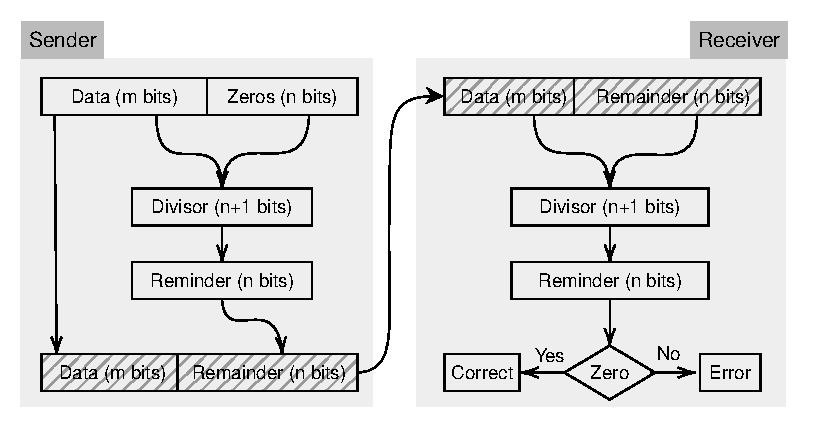
\includegraphics[scale=0.9]{figures/crc/crc_flow.pdf}
  \caption{The CRC error control processes}
  \label{fig:crc_flow}
\end{figure}


The binary polynomial falls in the finite field arithmetic \cite{carlitz1932}. The divisions of binary polynomials can essentially be considered as the \texttt{XOR} bitwise operations, which can be easily implemented and calculated by computers. Figure \ref{fig:crc_example} illustrates a CRC remainder calculation example.



\begin{figure}[ht]
  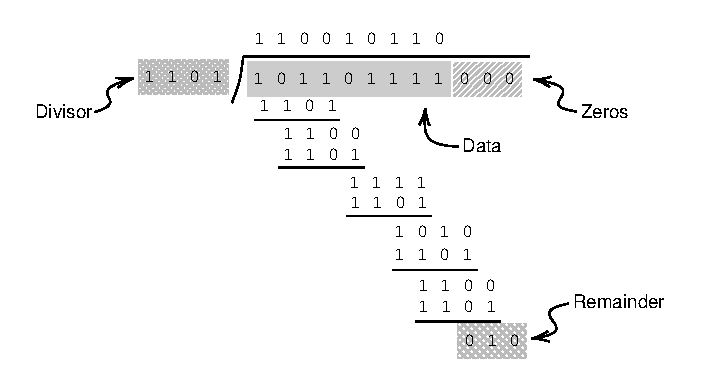
\includegraphics[scale=0.8]{figures/crc/crc_example.pdf}
  \caption{A CRC example with a 4-bit divisor and 3-bit remainder}
  \label{fig:crc_example}
\end{figure}


\section{ADS-B parity}

The polynomial form of the divisor (generator), $G(x)$, used for ADS-B (as well as other Mode~S messages) is \cite{gertz1984}:

\begin{equation}
  \begin{split}
  G(x) = &x^{24}+x^{23}+x^{22}+x^{21}+x^{20}+x^{19}+x^{18}+x^{17} \\
         &+x^{16}+x^{15}+x^{14}+x^{13}+x^{12}+x^{10}+x^{3}+1
  \end{split}
\end{equation}

This generator code was found by \cite{kasami1964}, which is known for its efficiency to correct burst errors. A 24-bit remainder is generated using this generator. It can also be written in different formats as:

\begin{verbatim}
Binary:   1111111111111010000001001
Decimal:  33551369
Octal:    177772011
HEX:      1FFF409
\end{verbatim}

Knowing the logic of CRC, the computation of the remainder and the verification of the error is fairly simple. Let  $x^{i}$ represent each bit of the message and $M(x)$ represent the polynomial corresponding to the ADS-B message, the CRC remainder (parity) $P(x)$ can thus be calculated as:

\begin{equation}
  \begin{split}
    M(x) &= \sum_{i=0}^{87} a_i x^i , \quad a_i \in (0, 1)\\
    P(x) &= M(x) ~ \% ~ G(x)
  \end{split}
\end{equation}

In the following pseudocode, the algorithm for computing the remainder of an ADS-B message is shown:

\begin{verbatim}
generator = 1111111111111010000001001

data_hex = 8D406B902015A678D4D220[000000]  # 11 + 3 zero bytes

data = 1000110101000000011010 1110010000001000000001  # 88 bits
       0101101001100111100011 0101001101001000100000
      [000000000000000000000000]  # append 24 zero bits

FOR i FROM 0 TO (112-24):
  IF data[i] IS 1:
    data[i:i+24] = data[i:i+24] XOR generator

remainder = data[-24:]

# final result: 101010100100101111011010, or AA4BDA in hexadecimal
\end{verbatim}

To check whether an error occurs in the message, replace the \texttt{data\_hex} in the previous example with the received message and run the same CRC process. The message is correct if all final 24 remainder bits are zeros.

\begin{notebox}{Try it out}
Using pyModeS, we can check the correctness of a ADS-B message as: 

\begin{verbatim}
import pyModeS as pms

msgA = "8D406B902015A678D4D220AA4BDA"
msgB = "8D4CA251204994B1C36E60A5343D"

remainderA = pms.crc(msgA)  # should be 0
remainderB = pms.crc(msgB)  # should be 16
\end{verbatim}

When the remainder is zero, the message is not corrupted. Otherwise, the error has occurred during the transmission.
\end{notebox}

\part{Decoding Mode~S}
\chapter{Basics of Mode S services} \label{chap:mode_s_basics}

In chapter \ref{chap:intro}, an overview of different Mode S services is given. Most of the services except the extended squitter are interrogations based, which means information is only transmitted upon request. The request, also known as \emph{uplink}, is transmitted using 1030 megahertz radio frequency. The reply (\emph{downlink}) signals are all transmitted using the 1090 megahertz radio frequency. Hence, all Mode S downlink messages can be intercepted using the same setup as ADS-B.

In the following chapters of this book, we are going to explain the interrogation based Mode S services in four groups, specifically:

\begin{enumerate}
  \item All-call reply (DF 11)
  \item ACAS short and long replies (DF 0/16)
  \item Altitude and identity replies (DF 4/5)
  \item Comm-B, with altitude and identity replies (DF 20/21)
    \begin{enumerate}
      \item Mode S elementary surveillance (ELS)
      \item Mode S enhanced surveillance (EHS)
      \item Meteorological information
    \end{enumerate}
\end{enumerate}

In this chapter, we discuss some of the common aspects regarding the decoding of Mode S messages. First of all, the structure of Mode S services is reviewed. Then, Mode S parity and ICAO address recovery are discussed. Finally, some common terminologies related to Comm-B messages are explained.


\section{Mode S message structures}

Based on Figure \ref{fig:mode_s_uplink_pulses} from the introduction chapter, we see that there are two types of Mode S messages in terms of message length. Table \ref{tb:mode_s_formats} indicates that among the current 11 different downlink formats, 4 are short messages consisting of 56 bits. The other 7 are long messages with 112 bits. All formats share the same structure of a header consisting of 5 bits format code and 24 bits parity at the end, as shown in the Figure \ref{fig:modes_msg_structures}.

\begin{figure}[!ht]
  \centering
  \scalebox{0.9}{
  \begin{tikzpicture}
    [
      graynode/.style={
        rectangle, draw=black!60, fill=black!5, thick, minimum size=6mm, font=\small
      },
      darkgraynode/.style={
        rectangle, draw=black!60, fill=black!15, thick, minimum size=6mm, font=\small
      },
    ]
   \node[darkgraynode] (df1) {DF:5};
   \node[graynode] (mb1) [right=-1pt of df1, minimum width=3cm] {27 bits};
   \node[darkgraynode] (pi1) [right=-1pt of mb1, minimum width=2.8cm] {Parity:24};

   \node[darkgraynode] (df2) [below=10pt of df1]{DF:5};
   \node[graynode] (mb2) [right=-1pt of df2, minimum width=9cm] {83 bits};
   \node[darkgraynode] (pi2) [right=-1pt of mb2, minimum width=2.8cm] {Parity:24};

  \end{tikzpicture}
  }
  \caption{The structures of Mode S short and long messages}
  \label{fig:modes_msg_structures}
\end{figure}




\section{Parity} \label{sec:parity}

Mode S uses three types of parity. The first one is what is used for ADS-B in the extended squitter (see chapter \ref{chap:adsb_parity}). The other two types of parities are Address Parity (AP) and Data Parity (DP).

For any type of Mode S messages, the parity can be calculated ass follows:

1) Let  $x^{i}$ represent each bit of the message and $M(x)$ represent the polynomial corresponding Mode S message, the parity $P(x)$ can thus be calculated as the CRC remainder:

\begin{equation} \label{eq:crc}
  \begin{split}
    M(x) &= \sum_{i=0}^{87~\mathrm{or}~32} a_i x^i , \quad a_i \in (0, 1)\\
    P(x) &= M(x) ~ \% ~ G(x)
  \end{split}
\end{equation}

2) For an extended squitter message, $P(x)$ is directly transmitted as the parity in the last 24 bits of the message. Errors can be detected by performing the same computation process at the receiving side when received parity differs from this newly computed remainder.

However, for other types of Mode S messages, \emph{Address Parity} (AP) is generated by overlaying the normal CRC remainder with the 24-bit transponder ICAO address. Thus, the final parity included in the message is not $P(x)$, but a new parity $P_A(x)$:

\begin{equation}
  P_A(x) = P(x) + A(x)
\end{equation}

\noindent where $A(x)$ is the polynomial representing the ICAO address of the transponder.

3) For some of the Downlink Format 20 and 21 Mode S messages, upon request of the SSR interrogation, another addition with the Comm-B Data Selector (BDS) number is performed \cite{gertz1984}. In this case, the \emph{Data Parity} (DP), is included in the last 24 bits of the Mode S message and transmitted.

When DP is in use, the parity is overlaid with the modified ICAO address, Modified AA (MA). The MA is calculated as the polynomial addition of ICAO address and BDS code (with 16 bits of zeros appended after), for example:

\begin{verbatim}
ICAO:         DD33AA      1101 1101 0011 0011 1010 1010
                                      XOR
BDS 4,4       440000      0100 0100 0000 0000 0000 0000
-------------------------------------------------------
Modified AA   9933AA      1001 1001 0011 0011 1010 1010
\end{verbatim}


Denote the modified address as $P_\mathrm{MA}(x)$ and the Data Parity as $P_D(x)$, the calculation is of $P_D(x)$ is:

\begin{equation}
  \begin{split}
    P_D(x) &= P(x) + P_\mathrm{MA}(x) \\
     &= P(x) + A(x) + D(x)
  \end{split}
\end{equation}

\noindent where $D(x)$ is the polynomial representing the BDS code of the Mode S Comm-B message.


\section{ICAO address recovery}

Since the interrogations are not known, information such as the transponder address is not known to third party receivers. The lack of this information makes error detection difficult.

For AP, the message parity field is produced by overlaying the direct parity with the transponder address. Hence, in order to recover the ICAO address, we can simply overlay the received parity (AP) with the parity calculated again from the payload data:

\begin{equation}
  A'(x) = P_A(x) + P(x)
\end{equation}

\noindent where $P_A(x)$ is the last 24-bit (assuming Address Parity) for the received message.

In order to demonstrate how to recover an ICAO address, we use the following example message:

\begin{verbatim}
Message:      A0001838CA380031440000F24177
------------------------------------------
Payload:      A0001838CA380031440000
------------------------------------------
Parity (AP):                        F24177
\end{verbatim}

In Figure \ref{fig:icao_revover}, the ICAO address recovering process is illustrated. We first use the Mode S CRC algorithm to compute the remainder (parity) from only the payload data \texttt{A0001838CA380031440000}. The remainder is found to be \texttt{CE2CA7}. Then, by performing the polynomial addition (XOR for bitwise operation) with the actual parity included in the message, the ICAO address can be computed as \texttt{3C6DD0}.

\begin{figure}[!ht]
  \centering
  \begin{tikzpicture}
    [
      datanode/.style={
        rectangle, draw=black!60, fill=black!10, thick, minimum size=6mm, font=\small, align=center
      },
      egnode/.style={
        rectangle, draw=black!60, fill=black!5, thick, minimum size=4mm, font=\footnotesize, align=center
      },
      operatornode/.style={
        draw=black!60, fill=black!20, thick, minimum size=6mm, font=\small, rounded corners=2mm
      },
    ]
   \node[datanode, text width=5cm] (msg) {Message without parity, $M(x)$};
   \node[egnode, text width=5cm] (msg-eg) [below=0pt of msg]{A0001838CA380031440000};

   \node[datanode, text width=2.5cm] (pi) [right=-1pt of msg] {Parity, $P_A(x)$};
   \node[egnode, text width=2.5cm] (pi-eg) [right=-1pt of msg-eg] {F24177};

   \node[operatornode] (crc) [below=15pt of msg-eg] {CRC, $M(x)\%G(x)$};
   \node[operatornode] (xor) [below=15pt of pi-eg] {+};

   \node[datanode, text width=3cm] (check) [below=50pt of msg-eg] {Remainder, $P(x)$};
   \node[egnode, text width=3cm] (check-eg) [below=0pt of check] {CE2CA7};

   \node[datanode, text width=2cm] (icao) [below=50pt of pi-eg] {ICAO, $A'(x)$};
   \node[egnode, text width=2cm] (icao-eg) [below=0pt of icao] {3C6DD0};

   \draw[->] (msg-eg) edge [thick, out=-90, in=90] (crc);
   \draw[->] (crc) edge [thick, out=-90, in=90] (check);
   \draw[->] (check) edge [thick, out=0, in=180] (xor);
   \draw[->] (pi-eg) edge [thick, out=-90, in=90] (xor);
   \draw[->] (xor) edge [thick, out=-90, in=90] (icao);

  \end{tikzpicture}

  \caption{The ICAO address recovery logic}
  \label{fig:icao_revover}
\end{figure}

For the cases of Data Parity, it is still possible to recover the transponder address using a similar process. However, we need to overlay again the previous result with the BDS code, assuming that the BDS code can be identified from the data:

\begin{equation}
  A'(x) = P_D(x) + P(x) + D(x)
\end{equation}


\noindent where $P_D(x)$ is the last 24-bit (assuming Data Parity) for the received message.

It is worth noting that in either case, the resulting $A'(x)$ is the same as the actual transponder address ($A(x)$) only if no error has occurred during the transmission. If the message is corrupted, the obtained address will be different from the actual one.

By combining with ICAO addresses obtained in ADS-B and other information independently decoded from Mode S message, this process can also be used for detecting Mode S errors as a third party observer. This method is described in \cite{sun2019pymodes}.

\begin{notebox}{Try it out}
Using \texttt{pyModeS}, we can obtain the ICAO address as: 

\begin{verbatim}
import pyModeS as pms

msg = "A0001838CA380031440000F24177"
icao = pms.icao(msg)
\end{verbatim}

\end{notebox}

\section{Two's complement coding} \label{sec:two_complement}

Two's complement coding is used for representing negative numbers in some Mode S messages, for example, heading and vertical rates in BDS 50 and BDS 60 messages. Every parameter in Mode S using two's complement coding include a 1-bit sign and n-bit value.

1) If the sign bit is \0, the result is simply the decimal representation of the value bits.

For example, we have the following representation of a signed parameter:

\begin{verbatim}
 sign    value
------------------
  0    111010011
\end{verbatim}

The result is the decimal representation of the last nine value bits, which is \texttt{467}.


2) If the sign bit is \1, we first calculate the decimal representation of the value bits ($x$) and then calculate the negative value as:

\begin{equation}
  x - 2^n
\end{equation}

For example, if we changed the signed bit in the previous example to \1, as follows:

\begin{verbatim}
 sign    value
------------------
  1    111010011
\end{verbatim}

since the sign bit is \1 and there are \texttt{9} value bits, the final value is calculated as:
\begin{equation}
  467 - 2^9 = -45
\end{equation}

\chapter{All-call reply}

Chapter \ref{chap:intro} shows that Mode~S all-call replies can be generated by Mode~S transponder to answer Mode~S-only all-call interrogations and Mode~A/C/S all-call interrogations.

Downlink format 11 is used for the all-call reply, and the length of the messages is 56 bits. The structure of an all-call reply message is quite simple. It only contains four fields, which are shown in Table \ref{tb:df11_structure}.

\begin{table}[ht]
\caption{All-call reply}
\label{tb:df11_structure}
\begin{tabular}{|l|l|l|l|}
\hline
\textbf{FIELD} & \textbf{} & \textbf{MSG} & \textbf{BITS} \\ \hline
Downlink format & DF & 1--5 & 5 \\ \hline
Capability & CA & 6--8 & 3 \\ \hline
Address announced & AA & 9--32 & 24 \\ \hline
Parity/interrogator identifier & PI & 33--56 & 24 \\ \hline
\end{tabular}
\end{table}

The fields can be decoded as follows:

\begin{itemize}
  \item The definition of transponder capability is the same as in ADS-B messages (Table \ref{tb:transponder_capability} in Chapter \ref{chap:adsb-basic}).

  \item The address refers to the 24-bit transponder address.

  \item The decoding of PI is similar to the decoding of ADS-B parity (Chapter \ref{chap:adsb_parity}). 
\end{itemize}

For a message with downlink format 11, PI is overlaid with the interrogator identifier.\footnote{In fact, PI in ADS-B is also overlaid with the interrogator identifier. However, since ADS-B is not interrogation-based, the identifier is set to 0. Thus, PI is always the same as the CRC remainder in ADS-B.} Hence, assuming there is no error in the data, the CRC will produce the interrogator identifier code for all-call replies.


A decoding example is shown as follows:

\begin{verbatim}
MSG HEX:  5D484FDEA248F5
MSG BIN:  01011   101    010010000100111111011110  101000100100100011110101
          [DF=11] [CA=5] [AA=484FDE]               [CRC=22]
\end{verbatim}

With the capability value (CA=5), we can see the aircraft has a Level 2+ transponder, with the ability to set CA to 7 and that it is airborne. The CRC remainder indicates the interrogator identifier code is 22.

\begin{notebox}{Try it out}
Using pyModeS, we can obtain the ICAO address as: 

\begin{verbatim}
import pyModeS as pms

msg = "5D484FDEA248F5"
pms.icao(msg)
\end{verbatim}

Output: 

\begin{verbatim}
484FDE
\end{verbatim}

\end{notebox}
\chapter{Surveillance replies} \label{chap:surv_reply}

Surveillance replies consist of short messages (56 bits) that respond to the selective interrogations of the secondary surveillance radar based on the 24-bit transponder addresses of the aircraft. Two types of information are transmitted: altitude (DF=4) and identity (DF=5).


\section{Message structure}

The structure of altitude and identity surveillance replies are similar, as shown in Tables \ref{tb:df_4_structure} and \ref{tb:df_5_structure}. The main difference is that bits 20 to 32 are used to encode either the altitude or the squawk code.

\begin{table}[ht]
  \centering
  \caption{Surveillance altitude reply (DF=4)}
  \label{tb:df_4_structure}
  \begin{tabular}[t]{|l|l|l|l|}
  \hline
  \textbf{FIELD} & \textbf{} & \textbf{MSG} & \textbf{BITS} \\ \hline
  Downlink format   & DF & 1-5    & 5   \\ \hline
  Flight status     & FS & 6-8    & 3   \\ \hline
  Downlink request  & DR & 9-13   & 5   \\ \hline
  Utility message   & UM & 14-19  & 6   \\ \hline
  Altitude code     & AC & 20-32  & 13  \\ \hline
  Address parity    & AP & 33-56  & 24  \\ \hline
  \end{tabular}
\end{table}

\begin{table}[ht]
  \centering
  \caption{Surveillance identity reply (DF=5)}
  \label{tb:df_5_structure}
  \begin{tabular}[t]{|l|l|l|l|}
  \hline
  \textbf{FIELD} & \textbf{} & \textbf{MSG} & \textbf{BITS} \\ \hline
  Downlink format   & DF & 1-5    & 5   \\ \hline
  Flight status     & FS & 6-8    & 3   \\ \hline
  Downlink request  & DR & 9-13   & 5   \\ \hline
  Utility message   & UM & 14-19  & 6   \\ \hline
  Identity code     & ID & 20-32  & 13  \\ \hline
  Address parity    & AP & 33-56  & 24  \\ \hline
  \end{tabular}
\end{table}
  

The definitions of the common fields are:

\begin{itemize}
  \item \emph{Flight status (FS)}: 3 bits, shows status of alert, special position pulse (SPI, in Mode~A only) and aircraft status (airborne or on-ground). The field is interpreted as:

  \begin{quote}
    \small
    \texttt{000}: no alert, no SPI, aircraft is airborne \\
    \texttt{001}: no alert, no SPI, aircraft is on-ground \\
    \texttt{010}: alert, no SPI, aircraft is airborne \\
    \texttt{011}: alert, no SPI, aircraft is on-ground \\
    \texttt{100}: alert, SPI, aircraft is airborne or on-ground \\
    \texttt{101}: no alert, SPI, aircraft is airborne or on-ground \\
    \texttt{110}: reserved \\
    \texttt{111}: not assigned
  \end{quote}

  \item \emph{Downlink request (DR)}: 5 bits, contains the type of request. In surveillance replies, only values 0, 1, 4, and 5 are used. The field can be decoded as:

  \begin{quote}
    \small
    \texttt{00000}: no downlink request \\
    \texttt{00001}: request to send Comm-B message \\
    \texttt{00100}: Comm-B broadcast message 1 available \\
    \texttt{00101}: Comm-B broadcast message 2 available
  \end{quote}

  \item \emph{Utility message (UM)}: 6 bits, contains transponder communication status information. 
  
  \begin{itemize}
    \item IIS: The first 4 bits of UM indicate the interrogator identifier code. 
    \item IDS: The last 2 bits indicate the type of reservation made by the interrogator.

    \begin{quote}
      \small
      \texttt{00}: no information \\
      \texttt{01}: IIS contains Comm-B interrogator identifier code \\
      \texttt{10}: IIS contains Comm-C interrogator identifier code \\
      \texttt{11}: IIS contains Comm-D interrogator identifier code \\
    \end{quote}
  
  \end{itemize}

  


\end{itemize}



\section{Altitude code} \label{sec:alt_code}

The 13-bit altitude code can be encoded in 25-ft increments, 100-ft increments, or in metric units (m). The 7th bit (MSG bit 28) is defined as the M bit. When the M bit is set to \0, the 9th bit (MSG bit 30) is defined as the Q bit.

The decoding rules are as follows:

\begin{itemize}
  \item When all bits are set to \0, altitude information is not available or invalid.

  \item When M=1, removing the M bit, the remaining 12 bits represent the altitude in meters.

  \item When M=0 and Q=1, removing the M and Q bits, the remaining 11 bits encode the altitude with 25 ft increments. Denote $N$ as the decimal value of the remaining 11 bits. The altitude is calculated as $25 \times N - 1000$ ft.

  \item When M=0 and Q=0, the remaining bits are defined as follows:

\begin{verbatim}
                                M        Q
+----+----+----+----+----+----+---+----+---+----+----+----+----+
| C1 | A1 | C2 | A2 | C4 | A4 | 0 | B1 | 0 | B2 | D2 | B4 | D4 |
+----+----+----+----+----+----+---+----+---+----+----+----+----+
\end{verbatim}

  This structure corresponds to the Mode~C altitude reply. This structure is used to encode altitudes above 50187.5 ft.

\end{itemize}

\begin{notebox}{Try it out}
Using \texttt{pyModeS}, we can calculate the altitude code as: 

\begin{verbatim}
import pyModeS as pms

msg = "2000171806A983"
altitude = pms.altcode(msg)  # 36000 (ft)
\end{verbatim}

\end{notebox}


\section{Identity code} \label{sec:id_code}

The 13-bit identity code encodes the 4 octal digit squawk code (from \texttt{0000} to \texttt{7777}). The structure of this field is shown as follows:

\begin{verbatim}
+----+----+----+----+----+----+---+----+----+----+----+----+----+
| C1 | A1 | C2 | A2 | C4 | A4 | X | B1 | D1 | B2 | D2 | B4 | D4 |
+----+----+----+----+----+----+---+----+----+----+----+----+----+
\end{verbatim}

The binary representation of the octal digit is:

\begin{verbatim}
A4 A2 A1 | B4 B2 B1 | C4 C2 C1 | D4 D2 D1
\end{verbatim}


Next, we will use an example to explain the decoding of the identity code. The example message is:

\begin{verbatim}
MSG HEX: 2A00516D492B80
MSG BIN: 00101 01000000000010 1000101101101 010010010010101110000000
         [DF=5]              [identity code]
\end{verbatim}

The binary identity code can be interpreted as follows:

\begin{verbatim}
C1 A1 C2 A2 C4 A4  X  B1 D1 B2 D2 B4 D4
1  0  0  0  1  0   1   1  0  1  1  0  1
\end{verbatim}

Rearranging the bits, we have three groups of binaries:
\begin{verbatim}
A4 A2 A1 | B4 B2 B1 | C4 C2 C1 | D4 D2 D1
0  0  0  | 0  1  1  | 1  0  1  | 1  1  0
\end{verbatim}

Finally, the four octal digit squawk code can be decoded from the binary groups as:
\begin{verbatim}
0 3 5 6
\end{verbatim}

\begin{notebox}{Try it out}
Using \texttt{pyModeS}, we can calculate the squawk code as: 

\begin{verbatim}
import pyModeS as pms

msg = "2A00516D492B80"
squawk = pms.idcode(msg)  # 0356
\end{verbatim}

\end{notebox}
\chapter{Airborne collision avoidance system}

\section{Background}

\emph{Airborne Collision Avoidance System} (ACAS) is a system to reduce the risk of mid-air collisions and near mid-air collisions between aircraft. There are three types of ACAS systems according to \cite{icaoA10V4}, which are:

\begin{itemize}
  \item ACAS I: Gives traffic advisories (TA), without recommending manoeuvres.
  \item ACAS II: Gives traffic advisories (TA) and resolution advisories (RA) only in vertical directions.
  \item ACAS III: Gives traffic advisories (TA) and resolution advisories (RA) in both horizontal and vertical directions. ACAS III is not currently implemented
\end{itemize}

This chapter will focus on ACAS II. The ACAS II is a system that utilizes the aircraft transponder, which interrogates the Mode~C and Mode~S transponders of nearby aircraft. When threats are detected, corresponding alerts are given to the pilots.

Currently, the most common implementation of ACAS II is \emph{Traffic alert and Collision Avoidance System} (TCAS) II version 7.1, which was initiated by EUROCONTROL. It has been mandatory for aircraft in Europe since 2015. ACAS II works independently of the navigation system, FMS, and ATC. No input from these systems is considered for producing the alerts.

In ACAS II, TA and RA are triggered when certain thresholds to the closest point of approach (CPA) are passed. The thresholds depend on the altitude, speed, and heading of the aircraft. The examples of the TA and RA regions are illustrated in Figure \ref{fig:acas_regions}.

\begin{figure}[ht]
  \centering
  

\tikzset{every picture/.style={line width=0.75pt}} %set default line width to 0.75pt        

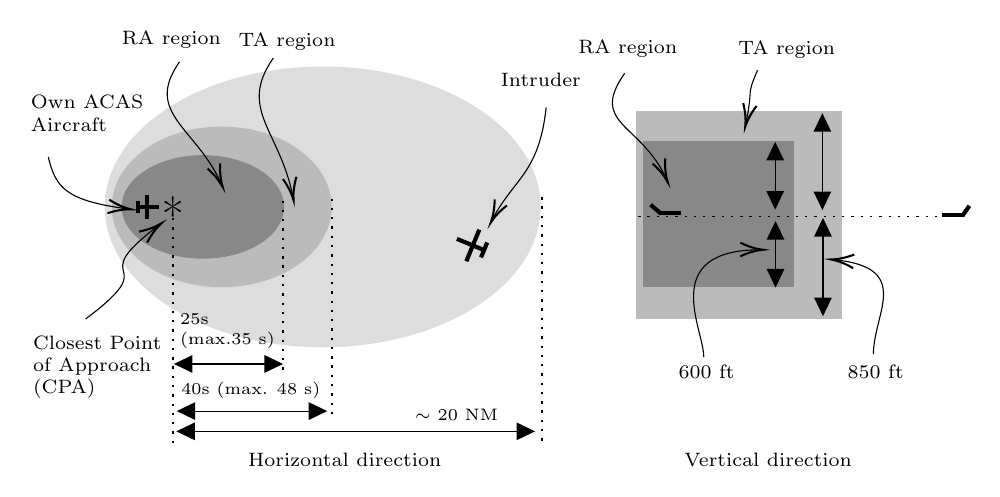
\begin{tikzpicture}[x=0.75pt,y=0.75pt,yscale=-1,xscale=1]
%uncomment if require: \path (0,300); %set diagram left start at 0, and has height of 300

%Shape: Rectangle [id:dp540037046483179] 
\draw  [draw opacity=0][fill={rgb, 255:red, 187; green, 187; blue, 187 }  ,fill opacity=1 ] (306.97,69.51) -- (406.37,69.51) -- (406.37,169.43) -- (306.97,169.43) -- cycle ;
%Shape: Ellipse [id:dp4377400846575308] 
\draw  [draw opacity=0][fill={rgb, 255:red, 221; green, 221; blue, 221 }  ,fill opacity=1 ] (51,115.63) .. controls (51,78.28) and (98.01,48) .. (156,48) .. controls (213.99,48) and (261,78.28) .. (261,115.63) .. controls (261,152.97) and (213.99,183.25) .. (156,183.25) .. controls (98.01,183.25) and (51,152.97) .. (51,115.63) -- cycle ;
%Shape: Ellipse [id:dp13502883869152638] 
\draw  [draw opacity=0][fill={rgb, 255:red, 187; green, 187; blue, 187 }  ,fill opacity=1 ] (54.37,115.63) .. controls (54.37,94.25) and (78.09,76.92) .. (107.35,76.92) .. controls (136.61,76.92) and (160.33,94.25) .. (160.33,115.63) .. controls (160.33,137) and (136.61,154.33) .. (107.35,154.33) .. controls (78.09,154.33) and (54.37,137) .. (54.37,115.63) -- cycle ;
%Shape: Ellipse [id:dp7716523443232073] 
\draw  [draw opacity=0][fill={rgb, 255:red, 136; green, 136; blue, 136 }  ,fill opacity=1 ] (59.13,115.63) .. controls (59.13,101.85) and (76.65,90.68) .. (98.27,90.68) .. controls (119.88,90.68) and (137.4,101.85) .. (137.4,115.63) .. controls (137.4,129.4) and (119.88,140.57) .. (98.27,140.57) .. controls (76.65,140.57) and (59.13,129.4) .. (59.13,115.63) -- cycle ;
%Straight Lines [id:da6234084719762716] 
\draw [line width=0.75]  [dash pattern={on 0.84pt off 2.51pt}]  (83.8,121.03) -- (83.8,231.25) ;
%Straight Lines [id:da986581977231834] 
\draw [line width=0.75]  [dash pattern={on 0.84pt off 2.51pt}]  (137,112.57) -- (137,194.25) ;
%Straight Lines [id:da017080809888795345] 
\draw [line width=0.75]  [dash pattern={on 0.84pt off 2.51pt}]  (160.33,111.63) -- (160.33,216.75) ;
%Straight Lines [id:da9044293647497716] 
\draw [line width=0.75]  [dash pattern={on 0.84pt off 2.51pt}]  (261.5,110.96) -- (261.5,230.25) ;
%Straight Lines [id:da8901469455802469] 
\draw    (87.33,191.29) -- (133.88,191.29) ;
\draw [shift={(136.88,191.29)}, rotate = 180] [fill={rgb, 255:red, 0; green, 0; blue, 0 }  ][line width=0.08]  [draw opacity=0] (8.93,-4.29) -- (0,0) -- (8.93,4.29) -- cycle    ;
\draw [shift={(84.33,191.29)}, rotate = 0] [fill={rgb, 255:red, 0; green, 0; blue, 0 }  ][line width=0.08]  [draw opacity=0] (8.93,-4.29) -- (0,0) -- (8.93,4.29) -- cycle    ;
%Straight Lines [id:da17855104123419885] 
\draw    (88.66,214) -- (155.2,214) ;
\draw [shift={(158.2,214)}, rotate = 180] [fill={rgb, 255:red, 0; green, 0; blue, 0 }  ][line width=0.08]  [draw opacity=0] (8.93,-4.29) -- (0,0) -- (8.93,4.29) -- cycle    ;
\draw [shift={(85.66,214)}, rotate = 0] [fill={rgb, 255:red, 0; green, 0; blue, 0 }  ][line width=0.08]  [draw opacity=0] (8.93,-4.29) -- (0,0) -- (8.93,4.29) -- cycle    ;
%Straight Lines [id:da48115516720549056] 
\draw    (88.48,223.76) -- (255.33,223.76) ;
\draw [shift={(258.33,223.76)}, rotate = 180] [fill={rgb, 255:red, 0; green, 0; blue, 0 }  ][line width=0.08]  [draw opacity=0] (8.93,-4.29) -- (0,0) -- (8.93,4.29) -- cycle    ;
\draw [shift={(85.48,223.76)}, rotate = 0] [fill={rgb, 255:red, 0; green, 0; blue, 0 }  ][line width=0.08]  [draw opacity=0] (8.93,-4.29) -- (0,0) -- (8.93,4.29) -- cycle    ;
%Curve Lines [id:da018523465484951096] 
\draw    (263.67,67.67) .. controls (260.16,99.65) and (248.28,101.59) .. (237.74,121.68) ;
\draw [shift={(236.93,123.27)}, rotate = 296.42] [color={rgb, 255:red, 0; green, 0; blue, 0 }  ][line width=0.75]    (10.93,-3.29) .. controls (6.95,-1.4) and (3.31,-0.3) .. (0,0) .. controls (3.31,0.3) and (6.95,1.4) .. (10.93,3.29)   ;
%Curve Lines [id:da6845841341175849] 
\draw    (132.24,43.9) .. controls (114.79,68.67) and (135.6,78.88) .. (141.68,110.96) ;
\draw [shift={(141.95,112.44)}, rotate = 260.25] [color={rgb, 255:red, 0; green, 0; blue, 0 }  ][line width=0.75]    (10.93,-3.29) .. controls (6.95,-1.4) and (3.31,-0.3) .. (0,0) .. controls (3.31,0.3) and (6.95,1.4) .. (10.93,3.29)   ;
%Curve Lines [id:da9696521875385951] 
\draw    (87,45.75) .. controls (69.64,70.39) and (94.85,77.27) .. (107.07,104.32) ;
\draw [shift={(107.8,106)}, rotate = 247.3] [color={rgb, 255:red, 0; green, 0; blue, 0 }  ][line width=0.75]    (10.93,-3.29) .. controls (6.95,-1.4) and (3.31,-0.3) .. (0,0) .. controls (3.31,0.3) and (6.95,1.4) .. (10.93,3.29)   ;
%Curve Lines [id:da6095777107453137] 
\draw    (41.8,169.6) .. controls (81.4,139.9) and (39.06,153.32) .. (77.02,124.49) ;
\draw [shift={(78.2,123.6)}, rotate = 503.13] [color={rgb, 255:red, 0; green, 0; blue, 0 }  ][line width=0.75]    (10.93,-3.29) .. controls (6.95,-1.4) and (3.31,-0.3) .. (0,0) .. controls (3.31,0.3) and (6.95,1.4) .. (10.93,3.29)   ;
%Curve Lines [id:da5170352565441036] 
\draw    (23.8,91.6) .. controls (27.33,106.5) and (32.39,112.56) .. (61.77,116.56) ;
\draw [shift={(63.6,116.8)}, rotate = 187.35] [color={rgb, 255:red, 0; green, 0; blue, 0 }  ][line width=0.75]    (10.93,-3.29) .. controls (6.95,-1.4) and (3.31,-0.3) .. (0,0) .. controls (3.31,0.3) and (6.95,1.4) .. (10.93,3.29)   ;
%Shape: Rectangle [id:dp533002490009195] 
\draw  [draw opacity=0][fill={rgb, 255:red, 136; green, 136; blue, 136 }  ,fill opacity=1 ] (310.19,83.79) -- (383,83.79) -- (383,154.3) -- (310.19,154.3) -- cycle ;
%Straight Lines [id:da8531155029939488] 
\draw  [dash pattern={on 0.84pt off 2.51pt}]  (308,120.2) -- (455.8,120.2) ;
%Straight Lines [id:da21045740389571743] 
\draw    (396.74,73.46) -- (396.74,114.14) ;
\draw [shift={(396.74,117.14)}, rotate = 270] [fill={rgb, 255:red, 0; green, 0; blue, 0 }  ][line width=0.08]  [draw opacity=0] (8.93,-4.29) -- (0,0) -- (8.93,4.29) -- cycle    ;
\draw [shift={(396.74,70.46)}, rotate = 90] [fill={rgb, 255:red, 0; green, 0; blue, 0 }  ][line width=0.08]  [draw opacity=0] (8.93,-4.29) -- (0,0) -- (8.93,4.29) -- cycle    ;
%Straight Lines [id:da39726982970462643] 
\draw    (397.03,123.97) -- (397.03,165.29) ;
\draw [shift={(397.03,168.29)}, rotate = 270] [fill={rgb, 255:red, 0; green, 0; blue, 0 }  ][line width=0.08]  [draw opacity=0] (8.93,-4.29) -- (0,0) -- (8.93,4.29) -- cycle    ;
\draw [shift={(397.03,120.97)}, rotate = 90] [fill={rgb, 255:red, 0; green, 0; blue, 0 }  ][line width=0.08]  [draw opacity=0] (8.93,-4.29) -- (0,0) -- (8.93,4.29) -- cycle    ;
%Straight Lines [id:da7836831316943322] 
\draw    (374,87.29) -- (374,113.91) ;
\draw [shift={(374,116.91)}, rotate = 270] [fill={rgb, 255:red, 0; green, 0; blue, 0 }  ][line width=0.08]  [draw opacity=0] (8.93,-4.29) -- (0,0) -- (8.93,4.29) -- cycle    ;
\draw [shift={(374,84.29)}, rotate = 90] [fill={rgb, 255:red, 0; green, 0; blue, 0 }  ][line width=0.08]  [draw opacity=0] (8.93,-4.29) -- (0,0) -- (8.93,4.29) -- cycle    ;
%Straight Lines [id:da8366254239434643] 
\draw    (374.17,125.46) -- (374.17,151.46) ;
\draw [shift={(374.17,154.46)}, rotate = 270] [fill={rgb, 255:red, 0; green, 0; blue, 0 }  ][line width=0.08]  [draw opacity=0] (8.93,-4.29) -- (0,0) -- (8.93,4.29) -- cycle    ;
\draw [shift={(374.17,122.46)}, rotate = 90] [fill={rgb, 255:red, 0; green, 0; blue, 0 }  ][line width=0.08]  [draw opacity=0] (8.93,-4.29) -- (0,0) -- (8.93,4.29) -- cycle    ;
%Straight Lines [id:da5952844140181097] 
\draw [line width=1.5]    (317.8,118.4) -- (328.4,118.4) ;
%Straight Lines [id:da8295175050930979] 
\draw [line width=1.5]    (314,114.6) -- (319,118.9) ;

%Straight Lines [id:da04092572822853335] 
\draw [line width=1.5]    (454.6,119.4) -- (465.2,119.4) ;
%Straight Lines [id:da5699307237098779] 
\draw [line width=1.5]    (467.6,115.1) -- (464.2,119.9) ;

%Straight Lines [id:da21934003742303032] 
\draw [line width=1.5]    (66.78,115.67) -- (77.12,115.67) ;
%Straight Lines [id:da0093763820452204] 
\draw [line width=1.5]    (66.99,112.91) -- (66.99,118.5) ;
%Straight Lines [id:da2881776632398887] 
\draw [line width=1.5]    (71.18,109.78) -- (71.18,121.56) ;

%Straight Lines [id:da1381529616415611] 
\draw [line width=1.5]    (234.02,136.54) -- (220.65,131.03) ;
%Straight Lines [id:da8623314816948788] 
\draw [line width=1.5]    (232.27,139.99) -- (235.25,132.76) ;
%Straight Lines [id:da20993063325707295] 
\draw [line width=1.5]    (225.19,141.8) -- (231.46,126.59) ;

%Curve Lines [id:da02921148242050675] 
\draw    (339.57,188) .. controls (339.97,175.33) and (317.18,136.5) .. (366.61,136.26) ;
\draw [shift={(368.13,136.27)}, rotate = 180.62] [color={rgb, 255:red, 0; green, 0; blue, 0 }  ][line width=0.75]    (10.93,-3.29) .. controls (6.95,-1.4) and (3.31,-0.3) .. (0,0) .. controls (3.31,0.3) and (6.95,1.4) .. (10.93,3.29)   ;
%Curve Lines [id:da26674369247427876] 
\draw    (421.33,186.5) .. controls (421.39,166.69) and (440.42,144.95) .. (402.7,141.11) ;
\draw [shift={(400.93,140.95)}, rotate = 364.76] [color={rgb, 255:red, 0; green, 0; blue, 0 }  ][line width=0.75]    (10.93,-3.29) .. controls (6.95,-1.4) and (3.31,-0.3) .. (0,0) .. controls (3.31,0.3) and (6.95,1.4) .. (10.93,3.29)   ;
%Curve Lines [id:da6549261187856048] 
\draw    (301.5,51.25) .. controls (284.14,75.89) and (309.25,75.18) .. (321.47,101.93) ;
\draw [shift={(322.2,103.6)}, rotate = 247.3] [color={rgb, 255:red, 0; green, 0; blue, 0 }  ][line width=0.75]    (10.93,-3.29) .. controls (6.95,-1.4) and (3.31,-0.3) .. (0,0) .. controls (3.31,0.3) and (6.95,1.4) .. (10.93,3.29)   ;
%Curve Lines [id:da058237463472115] 
\draw    (365.5,49.75) .. controls (359.82,62.9) and (363.61,57.09) .. (359.93,75.25) ;
\draw [shift={(359.57,77)}, rotate = 281.93] [color={rgb, 255:red, 0; green, 0; blue, 0 }  ][line width=0.75]    (10.93,-3.29) .. controls (6.95,-1.4) and (3.31,-0.3) .. (0,0) .. controls (3.31,0.3) and (6.95,1.4) .. (10.93,3.29)   ;

% Text Node
\draw (240.6,49.8) node [anchor=north west][inner sep=0.75pt]  [font=\scriptsize] [align=left] {Intruder};
% Text Node
\draw (110.13,185) node [anchor=south] [inner sep=0.75pt]  [font=\fontsize{0.6em}{0.72em}\selectfont] [align=left] {25s\\(max.35 s)};
% Text Node
\draw (121.35,209.34) node [anchor=south] [inner sep=0.75pt]  [font=\fontsize{0.6em}{0.72em}\selectfont] [align=left] {40s (max. 48 s)};
% Text Node
\draw (220.41,219.74) node [anchor=south] [inner sep=0.75pt]  [font=\fontsize{0.6em}{0.72em}\selectfont] [align=left] {$\displaystyle \sim $ 20 NM};
% Text Node
\draw (114.23,30.54) node [anchor=north west][inner sep=0.75pt]  [font=\scriptsize] [align=left] {TA region};
% Text Node
\draw (57.99,29.54) node [anchor=north west][inner sep=0.75pt]  [font=\scriptsize] [align=left] {RA region};
% Text Node
\draw (15.19,176.41) node [anchor=north west][inner sep=0.75pt]  [font=\scriptsize] [align=left] {Closest Point \\of Approach\\(CPA)};
% Text Node
\draw (14.12,60.79) node [anchor=north west][inner sep=0.75pt]  [font=\scriptsize] [align=left] {Own ACAS\\Aircraft};
% Text Node
\draw (326.17,190.48) node [anchor=north west][inner sep=0.75pt]  [font=\scriptsize] [align=left] {600 ft};
% Text Node
\draw (407.66,190.45) node [anchor=north west][inner sep=0.75pt]  [font=\scriptsize] [align=left] {850 ft};
% Text Node
\draw (329,233) node [anchor=north west][inner sep=0.75pt]  [font=\scriptsize] [align=left] {Vertical direction};
% Text Node
\draw (83.8,119.43) node  [font=\LARGE] [align=left] {*};
% Text Node
\draw (277.89,34.04) node [anchor=north west][inner sep=0.75pt]  [font=\scriptsize] [align=left] {RA region};
% Text Node
\draw (354.96,34.54) node [anchor=north west][inner sep=0.75pt]  [font=\scriptsize] [align=left] {TA region};
% Text Node
\draw (118.8,233) node [anchor=north west][inner sep=0.75pt]  [font=\scriptsize] [align=left] {Horizontal direction};


\end{tikzpicture}

  \caption{Example of an ACAS protection volume in horizontal and vertical directions (between FL50 and FL100)}
  \label{fig:acas_regions}
\end{figure}




\section{ACAS with Mode~C transponders}

ACAS system uses Mod C only all-call interrogation (see Figure \ref{fig:mode_s_inter_mode} in chapter \ref{chap:intro}) to detect aircraft that are only equipped with Mode~A/C transponders. In this case, the ACAS system initiates a sequence of interrogations with increasing power.

The interrogation pulse is slightly different from a Mode~A/C-only all-call interrogation. A special $S_1$ pulse (also known as "whisper-shout") is designed to reduce interference. The $S_1$ pulse is inserted 2 $\mu s$ ($\pm 0.15 \mu s$) before the $P_1$ pulse.

The reply should be sent with the following rules:

\begin{itemize}
  \item With both $S_1$ and $P_1$ above the minimum triggering level (MTL), no reply will be generated.
  \item With both $S_1$ and $P_1$ at MTL, the transponder will respond to 10\% of the interrogations.
  \item With $P_1$ at MTL and $S_1$ at MTL - 3 dB, the transponder will respond to 70\% of the interrogations.
  \item With $P_1$ at MTL and $S_1$ at MTL - 6 dB, the transponder will respond to 90\% of the interrogations.
\end{itemize}

\section{ACAS with Mode~S transponders}

For Mode~S transponders, ACAS system employs a three-phase process, which includes the phases of \emph{detection}, \emph{surveillance}, and \emph{coordination}.

For the detection phase, ACAS passively listens to Mode~S only all-call replies (DF=11). These all-call replies are usually generated as a result of ground SSR interrogations or as spontaneous replies. In this process, aircraft with Mode~S transponders in the vicinity are discovered. ACAS may also listen to extended squitter messages (Downlink Format 17, ADS-B) to detect other aircraft.

Once an aircraft is determined to be within the ACAS surveillance range, and within 10,000 ft of the own ACAS aircraft, ACAS will initiate a short air-air interrogation (UF=11) to acquire the range. The interrogation rate is defined as:

\begin{itemize}
  \item Once every five cycles: when the target aircraft maintains in the surveillance range.
  \item Once every cycle: when the target aircraft is within 3 NM or with time to closest approach less than 60 s.
\end{itemize}


The surveillance interrogation is stopped when all the following conditions are met:

\begin{itemize}
  \item A reply (DF=11) is received
  \item Both aircraft are below 18,000 ft.
  \item Target aircraft is more than 3 NM and 60 s away from the closest point of approach.
\end{itemize}


In Table \ref{tb:acas_uf_df_0}, fields for ACAS surveillance interrogation and reply messages are listed.

\begin{table}[ht]
\caption{ACAS surveillance uplink and downlink messages}
\label{tb:acas_uf_df_0}

\begin{subtable}[t]{0.7\linewidth}
  \centering
  \caption{Interrogation (uplink), UF=0}
  \begin{tabular}[t]{|l|l|l|l|}
  \hline
  \textbf{FIELD} & \textbf{} & \textbf{MSG} & \textbf{BITS} \\ \hline
  Uplink Format & UF & 1-5 & 5 \\ \hline
  Reserved &  & 6-8 & 3 \\ \hline
  Reply length & RL & 9 & 1 \\ \hline
  Reserved &  & 10-13 & 4 \\ \hline
  Acquisition & AQ & 14 & 1 \\ \hline
  Data selector & DS & 15-22 & 8 \\ \hline
  Reserved &  & 23-32 & 10 \\ \hline
  Address parity & AP & 33-56 & 24 \\ \hline
  \end{tabular}
\end{subtable}%

\vspace{0.5cm}

\begin{subtable}[t]{0.7\linewidth}
  \centering
  \caption{Reply (downlink), DF=0}
  \begin{tabular}[t]{|l|l|l|l|}
  \hline
  \textbf{FIELD} & \textbf{} & \textbf{MSG} & \textbf{BITS} \\ \hline
  Downlink Format & DF & 1-5 & 5 \\ \hline
  Vertical status & VS & 6 & 1 \\ \hline
  Cross-link capability & CC & 7 & 1 \\ \hline
  Reserved &  & 8 & 1 \\ \hline
  Sensitivity level & SL & 9-11 & 3 \\ \hline
  Reserved &  & 12-13 & 2 \\ \hline
  Reply information & RI & 14-17 & 4 \\ \hline
  Reserved &  & 18-19 & 2 \\ \hline
  Altitude code & AC & 20-32 & 13 \\ \hline
  Address parity & AP & 33-56 & 24 \\ \hline
  \end{tabular}
\end{subtable}

\end{table}


Once the target aircraft is within the RA region (a threat), ACAS initiates the coordination interrogation (UF=16). In this step, resolution information are transmitted and received through coordination replies (DF=16). Information that is included in both coordination messages is shown in Table \ref{tb:acas_uf_df_16}.


\begin{table}[ht]

\caption{ACAS coordination messages}
\label{tb:acas_uf_df_16}
\begin{subtable}[t]{0.7\linewidth}
  \centering
  \caption{Interrogation (UF=16)}
  \begin{tabular}[t]{|l|l|l|l|}
  \hline
  \textbf{FIELD} & \textbf{} & \textbf{MSG} & \textbf{BITS} \\ \hline
  Uplink Format & UF & 1-5 & 5 \\ \hline
  Reserved &  & 6-8 & 3 \\ \hline
  Reply length & RL & 9 & 1 \\ \hline
  Reserved &  & 10-13 & 4 \\ \hline
  Acquisition & AQ & 14 & 1 \\ \hline
  Reserved &  & 15-32 & 18 \\ \hline
  Message, U & MU & 33-88 & 56 \\ \hline
  Address parity & AP & 33-56 & 24 \\ \hline
  \end{tabular}
\end{subtable}%

\vspace{0.5cm}

\begin{subtable}[t]{0.7\linewidth}
  \centering
  \caption{Reply (DF=16)}
  \begin{tabular}[t]{|l|l|l|l|}
  \hline
  \textbf{FIELD} & \textbf{} & \textbf{MSG} & \textbf{BITS} \\ \hline
  Downlink Format & DF & 1-5 & 5 \\ \hline
  Vertical status & VS & 6 & 1 \\ \hline
  Reserved &  & 7-8 & 2 \\ \hline
  Sensitivity level & SL & 9-11 & 3 \\ \hline
  Reserved &  & 12-13 & 2 \\ \hline
  Reply information & RI & 14-17 & 4 \\ \hline
  Reserved &  & 18-19 & 2 \\ \hline
  Altitude code & AC & 20-32 & 13 \\ \hline
  Message, V & MV & 33-88 & 56 \\ \hline
  Address parity & AP & 89-112 & 24 \\ \hline
  \end{tabular}
\end{subtable}
\end{table}


Specific fields in above messages are defined as follows:

\begin{itemize}
  \item \emph{Reply length (RL)}: 1 bit, defines the required reply format: \0 requires a reply with DF=0, while \1 requires reply with DF=16.

  \item \emph{Acquisition (AQ)}: 1 bit, contains code that controls the content of RI field in the reply.

  \item \emph{Data selector (DS)}: 8 bits, indicates the BDS code of the MV content in reply with DF=16.

  \item \emph{Vertical status (VS)}: 1 bit, indicates whether the aircraft is airborne (\0) or on the ground (\1).

  \item \emph{Cross-link capability (CC)}: 1 bit, refers to the capability of reply DF=16 upon request of UF=0. When this 1-bit field is set to \1, the cross-link is supported. Otherwise, the field is set to \0.

  \item \emph{Sensitivity level (SL)}: 3 bits, represents the sensitivity level of the ACAS system. \0 indicates the ACAS is inoperative. Other values indicate the sensitivity level.

  \item \emph{Reply information (RI)}: 4 bits, indicates the type of reply to interrogating aircraft. For ACAS message, valid values are 0 and from 2 to 4. Other values are not part of the ACAS:

  \begin{quote}
    \texttt{0000}: No operating ACAS \\
    \texttt{0010}: ACAS with resolution capability inhibited \\
    \texttt{0011}: ACAS with vertical-only resolution capability \\
    \texttt{0111}: ACAS with vertical and horizontal resolution capability
  \end{quote}

  \item \emph{Altitude Code (AC)}: 13 bits, encodes the altitude of the aircraft. It can be decoded according to section \ref{sec:alt_code}.

\end{itemize}



\section{Message fields of ACAS coordination messages}


Message U-definition (MU) and Message V-definition (MV) are transmitted in ACAS coordination interrogation and reply messages, respectively. MU is used to transit resolution, ACAS broadcast, and RA broadcast. MV is used for reply purposes.

\subsection{MU (U-definition)}

\subsubsection{MU of ACAS resolution message}

When ACAS resolution information is transmitted in the UF=16 message, the first 8 bits of MU, U-definition subfields (UDS), is set to \texttt{0011 0000} (UDS=3,0). The corresponding fields are indicated in Table \ref{tb:acas_mu_uds30}.

\begin{table}[ht]
\caption{UF=16, MU for ACAS resolution messages, UDS=3,0}
\label{tb:acas_mu_uds30}
\begin{tabular}{|l|l|l|l|l|}
\hline
\textbf{FIELD} & \textbf{} & \textbf{MSG} & \textbf{MU} & \textbf{BITS} \\ \hline
U-definition subfield 1 [0011] & UDS1 & 33-36 & 1-4 & 4 \\ \hline
U-definition subfield 2 [0000] & UDS2 & 37-40 & 5-8 & 4 \\ \hline
Reserved &  & 41 & 9 & 1 \\ \hline
Multiple threat bit & MTB & 42 & 10 & 1 \\ \hline
Cancel vertical RAC & CVC & 43-44 & 11-12 & 2 \\ \hline
Vertical RAC & VRC & 45-46 & 13-14 & 2 \\ \hline
Cancel Horizontal RAC & CHC & 47-49 & 15-17 & 3 \\ \hline
Horizontal RAC & HRC & 50-52 & 18-20 & 3 \\ \hline
Reserved &  & 53-55 & 21-23 & 3 \\ \hline
Horizontal sense bits & HSB & 56-60 & 24-28 & 5 \\ \hline
Vertical sense bits & VSB & 61-64 & 29-32 & 4 \\ \hline
Aircraft address & MID & 65-88 & 33-56 & 24 \\ \hline
\end{tabular}
\end{table}

The significance of fields are listed as follows:

\begin{itemize}
  \item \emph{Multiple threat bit (MTB)}: 1 bit, indicates whether multiple threats are present.

  \item \emph{Vertical RAC \footnote{RAC: Resolution Advisory Complement} (VRC)}: 2 bits, contains vertical resolution advisory complement information:
  \begin{quote}
    \small
    \texttt{00}: No vertical RAC information \\
    \texttt{01}: Do not pass below \\
    \texttt{10}: Do not pass above \\
    \texttt{11}: Not assigned
  \end{quote}

  \item \emph{Cancel vertical RAC (CVC)}: 2 bits, cancels previously sent VRC:
  \begin{quote}
    \small
    \texttt{00}: No cancellation information \\
    \texttt{01}: Cancel "Do not pass below" \\
    \texttt{10}: Cancel "Do not pass above" \\
    \texttt{11}: Not assigned
  \end{quote}

  \item \emph{Horizontal RAC (HRC)}: 3 bits, contains horizontal resolution advisory complementary information:
  \begin{quote}
    \small
    \texttt{000}: No information\\
    \texttt{001}: Other ACAS sense is turn left; do not turn left \\
    \texttt{010}: Other ACAS sense is turn left; do not turn right \\
    \texttt{101}: Other ACAS sense is turn right; do not turn left \\
    \texttt{110}: Other ACAS sense is turn right; do not turn right \\
    \texttt{other}: Not assigned
  \end{quote}

  \item \emph{Cancel horizontal RAC (CHC)}: 3 bits, cancels previously sent HRC:
  \begin{quote}
    \small
    \texttt{000}: No cancellation information \\
    \texttt{001}: Cancel "Do not turn left" \\
    \texttt{010}: Cancel "Do not turn right" \\
    \texttt{other}: Not assigned
  \end{quote}

  \item \emph{Horizontal sense bits (HSB)}: 5 bits, uses Hamming code with an extra parity bit to detect errors (up to 3 bits) in CHC and HRC fields.

  \item \emph{Vertical sense bits (VSB)}: 4 bits, uses Hamming code with an extra parity bit to detect errors (up to 3 bits) in CVC and VRC fields.

  \item \emph{Aircraft address (MID)}: 24 bits, contains the 24-bits aircraft transponder address of the interrogating ACAS aircraft.

\end{itemize}



\subsubsection{MU of RA broadcast message} \label{sec:acas_ra}

When UF=16 is used for RA broadcast, UDS is set to \texttt{0011 0001} (UDS=3,1). The corresponding fields are indicated in Table \ref{tb:acas_mu_uds31}.

\begin{table}[ht]
\caption{UF=16, MU for RA broadcast, UDS=3,1}
\label{tb:acas_mu_uds31}
\begin{tabular}{|l|l|l|l|l|}
\hline
\textbf{FIELD} & \textbf{} & \textbf{MSG} & \textbf{MU} & \textbf{BITS} \\ \hline
U-definition subfield 1 [0011] & UDS1 & 33-36 & 1-4 & 4 \\ \hline
U-definition subfield 2 [0001] & UDS2 & 37-40 & 5-8 & 4 \\ \hline
Active RAs & ARA & 41-54 & 9-22 & 14 \\ \hline
RAC's record & RAC & 55-58 & 23-26 & 4 \\ \hline
RA terminated indicator & RAT & 59 & 27 & 1 \\ \hline
Multiple threat encounter & MTE & 60 & 28 & 1 \\ \hline
Reserved &  & 61-62 & 29-30 & 2 \\ \hline
Mode~A identity code & AID & 63-75 & 31-43 & 13 \\ \hline
Mode~C altitude code & CAC & 76-88 & 44-56 & 13 \\ \hline
\end{tabular}
\end{table}

The significance of fields are listed as follows:

\begin{itemize}
  \item \emph{Active RA (ARA)}: 14 bits, indicates the resolution advisory characteristics. It has to be interpreted together with the MTB field.

    \begin{itemize}
      \item When ARA first bit (MSG bit 41) is \1 and MTE is either \0 or \1:

      \begin{quote}
        \small
        Bit 42: RA is corrective (\1) or preventive (\0) \\
        Bit 43: RA is downward sense (\1) or upward sense (\0) \\
        Bit 44: RA is increased rate (\1) or not (\0) \\
        Bit 45: RA is a sense reversal (\1) or not (\0) \\
        Bit 46: RA is altitude crossing (\1) or not (\0) \\
        Bit 47: RA is positive (\1) or vertical speed limit (\0) \\
        Bit 48-54: Reserved for ACAS III
      \end{quote}

      \item When ARA first bit (MSG bit 41) is \0 and MTE is \1:

      \begin{quote}
        \small
        Bit 42: RA requires a correction in the upward sense (\1) or not (\0) \\
        Bit 43: RA requires a positive climb (\1) or not (\0) \\
        Bit 44: RA requires a correction in the downward sense (\1) or not (\0) \\
        Bit 45: RA requires a positive descent (\1) or not (\0) \\
        Bit 46: RA requires a crossing (\1) or not (\0) \\
        Bit 47: RA is a sense reversal (\1) or not (\0) \\
        Bit 48-54: Reserved for ACAS III
      \end{quote}

      \item When ARA first bit (MSG bit 41) is \0 and MTE is \0, no vertical RA is generated.
    \end{itemize}


  \item \emph{RAC's record (RAC)}: 4 bits, contains current active RACs that are received from other ACAS aircraft (if any). Each of the four bits in this field indicates the following RAC when set to \1. When a bit is set to \0, the corresponding RAC is inactive.

  \begin{quote}
    \small
    Bit 55: Do not pass below \\
    Bit 56: Do not pass above \\
    Bit 57: Do not pass left \\
    Bit 58: Do not pass right
  \end{quote}


  \item \emph{RA terminated indicator (RAT)}: 1 bit, indicates whether ACAS is currently generating RA in the ARA field or RA in the ARA field has been terminated.\footnote{The Mode~S transponder is still required to report RA 18 seconds after it is terminated by ACAS. Hence, the RAT field is used.}


  \item \emph{Multiple threat encounter (MTE)}: 1 bit, indicates whether multiple threats are currently being processed by the ACAS resolution. When MTE is set to \0, either one threat is being processed (ARA bit 41 sets to \1) or no threat is being processed (ARA bit 41 sets to \0). When MTE is set to \1, multiple threats are being processed.

  \item \emph{Mode~A identity code (AID)}: 13 bits, contains the Mode~A identity code (sqwake code) of the reporting aircraft. It can be decoded according to section \ref{sec:id_code}.

  \item \emph{Mode~C altitude code (CAC)}: 13 bits, contains the Mode~C altitude code reporting aircraft. It can be decoded according to section \ref{sec:alt_code}.


\end{itemize}



\subsubsection{MU of ACAS broadcast message}

When UF=16 is used for ACAS broadcast, UDS is set to \texttt{0011 0010} (UDS=3,2). The corresponding fields are indicated in Table \ref{tb:acas_mu_uds32}.

\begin{table}[ht]
\caption{UF=16, MU for ACAS broadcast, UDS=3,1}
\label{tb:acas_mu_uds32}
\begin{tabular}{|l|l|l|l|l|}
\hline
\textbf{FIELD} & \textbf{} & \textbf{MSG} & \textbf{MU} & \textbf{BITS} \\ \hline
U-definition subfield 1 [0011] & UDS1 & 33-36 & 1-4 & 4 \\ \hline
U-definition subfield 2 [0010] & UDS2 & 37-40 & 5-8 & 4 \\ \hline
Reserved &  & 41-64 & 9-32 & 24 \\ \hline
Aircraft address & MID & 65-8 & 33-56 & 24 \\ \hline
\end{tabular}
\end{table}

The only information that is broadcast in the MU of this message is the 24-bit transponder address of the interrogating aircraft.


\subsection{MV (V-definition)}

Similar to MU in the UF=16 message, MV in the DF=16 message contains a few common fields. The corresponding fields are indicated in Table \ref{tb:acas_mv_vds30}.

\begin{table}[ht]
\caption{DF=16, MV for coordinated reply, VDS=3,0}
\label{tb:acas_mv_vds30}
\begin{tabular}{|l|l|l|l|l|}
\hline
\textbf{FIELD} & \textbf{} & \textbf{MSG} & \textbf{MU} & \textbf{BITS} \\ \hline
V-definition subfield 1 [0011] & VDS1 & 33-36 & 1-4 & 4 \\ \hline
V-definition subfield 2 [0001] & VDS2 & 37-40 & 5-8 & 4 \\ \hline
Active RAs & ARA & 41-54 & 9-22 & 14 \\ \hline
RAC's record & RAC & 55-58 & 23-26 & 4 \\ \hline
RA terminated indicator & RAT & 59 & 27 & 1 \\ \hline
Multiple threat encounter & MTE & 60 & 28 & 1 \\ \hline
Reserved &  & 61-88 & 29-56 & 28 \\ \hline
\end{tabular}
\end{table}

We can see that the structure of the MV fields is similar to MU fields of RA broadcast (UDS=3,1) from Table \ref{tb:acas_mu_uds31}. The interpretations of these fields are also the same as in section \ref{sec:acas_ra}.

\chapter{Comm-B} \label{chap:comm-b}

Comm-B messages count for a large portion of the Mode~S selective interrogation responses. The message can have a downlink format of either 20 or 21, depending on whether the aircraft identity code or altitude code is included in the message.

Comm-B protocol supports many different types of messages (up to 255). Several important surveillance services utilize some of the Comm-B message types (see Figure \ref{fig:mode_s_services} from Chapter \ref{chap:intro}). In this book, we are mainly interested in three types of services, which are Mode~S Elementary Surveillance (ELS), Mode~S Enhanced Surveillance (EHS), and Meteorological information. By decoding these messages, we can discover some additional information of an aircraft.


\section{Structure}

Comm-B messages have similar structures as surveillance replies (DF=4/5). The structures are shown in the Tables \ref{tb:df_20_structure} and \ref{tb:df_21_structure}.

\begin{table}[!ht]
  \centering
  \caption{Comm-B, altitude reply (DF=20)}
  \label{tb:df_20_structure}
  \begin{tabular}[t]{|l|l|l|l|}
  \hline
  \textbf{FIELD} & \textbf{} & \textbf{MSG} & \textbf{BITS} \\ \hline
  Downlink format         & DF & 1--5    & 5   \\ \hline
  Flight status           & FS & 6--8    & 3   \\ \hline
  Downlink request        & DR & 9--13   & 5   \\ \hline
  Utility message         & UM & 14--19  & 6   \\ \hline
  Altitude code           & AC & 20--32  & 13  \\ \hline
  Message, Comm-B         & MB & 33--88  & 56  \\ \hline
  Parity  &  & 89--112  & 24  \\ \hline
  \end{tabular}
\end{table}


\begin{table}[ht]
  \centering
  \caption{Comm-B, identity reply (DF=21)}
  \label{tb:df_21_structure}
  \begin{tabular}[t]{|l|l|l|l|}
  \hline
  \textbf{FIELD} & \textbf{} & \textbf{MSG} & \textbf{BITS} \\ \hline
  Downlink format         & DF & 1--5    & 5   \\ \hline
  Flight status           & FS & 6--8    & 3   \\ \hline
  Downlink request        & DR & 9--13   & 5   \\ \hline
  Utility message         & UM & 14--19  & 6   \\ \hline
  Identity code           & ID & 20--32  & 13  \\ \hline
  Message, Comm-B         & MB & 33--88  & 56  \\ \hline
  Parity  &  & 89--112  & 24  \\ \hline
  \end{tabular}
\end{table}

The definitions of these common fields are the same as surveillance replies in Chapter \ref{chap:surv_reply}. In addition, depending on the request in the uplink, either address parity or data parity (see Chapter \ref{chap:mode_s_basics}) can be included in the downlink message.


\section{BDS}

Comm-B Data Selector (BDS) is an 8-bit code that determines which information to be included in the MB fields. It is often shown as a 2-digit hexadecimal, for example, \texttt{4,0} or \texttt{0,A}. We can make a comparison between the BDS code and Type Code used in ADS-B. They both help to identify which structure shall be used to decode the message, except that the BDS code is only included in the uplink (Comm-A). For Comm-B messages, BDS codes are not always included.

Without knowing the BDS code of the downlink message, the information contained in the MB field cannot be decoded. Fortunately, there are methods available that can be used to infer the BDS code for most of the messages and decode them. In later Chapter \ref{chap:bds_infer}, the inference process will be explained.

The following is the list of BDS codes for messages that will be discussed in detail in the different chapters.

\begin{itemize}
  \item BDS 1,0 - Data link capability report
  \item BDS 1,7 - Common usage GICB capability report
  \item BDS 2,0 - Aircraft identification
  \item BDS 3,0 - ACAS active resolution advisory
  \item BDS 4,0 - Selected vertical intention
  \item BDS 5,0 - Track and turn report
  \item BDS 6,0 - Heading and speed report
  \item BDS 4,4 - Meteorological routine air report
  \item BDS 4,5 - Meteorological hazard report
\end{itemize}

Here, the first four BDS codes (\texttt{1,0}, \texttt{1,7}, \texttt{2,0}, \texttt{3,0}) belong to the ELS service, the next three ones (\texttt{4,0}, \texttt{5,0}, \texttt{6,0}) belong to the EHS services, and the last two codes (\texttt{4,4}, \texttt{4,5}) report meteorological information. All ELS, EHS and meteorological services are discussed in the following chapters.

It is also worth noting that even ADS-B messages belong to Mode~S extended squitter, they are still assigned with BDS codes. The list of BDS codes for these ADS-B messages are:

\begin{itemize}
  \item BDS 0,5 - Extended squitter airborne position
  \item BDS 0,6 - Extended squitter surface position
  \item BDS 0,7 - Extended squitter status
  \item BDS 0,8 - Extended squitter identification and category
  \item BDS 0,9 - Extended squitter airborne velocity information
\end{itemize}
\chapter{Mode~S elementary surveillance}

Mode~S Elementary Surveillance (ELS) provides a set of basic functionalities that are supported by the Mode~S transponders. These basic functionalities include the reporting  of aircraft identity, altitude, transponder capability, and flight status. The set of BDS codes included in ELS are \texttt{1,0}, \texttt{1,7}, \texttt{2,0}, and \texttt{3,0}.

\section{Data link capability report (BDS 1,0)}

This message is designed to report the data link capability of the installed Mode~S transponder. Table \ref{tb:bds10} shows all fields in this message.

\begin{table}[ht]
\centering
\caption{Data link capability report (BDS 1,0), MB field}
\label{tb:bds10}
\begin{tabular}{|l|l|l|l|}
\hline
\textbf{FIELD} & \textbf{MSG} & \textbf{MB} & \textbf{BITS} \\ \hline
BDS Code {[}0001 0000{]} & 33--40 & 1--8 & 8 \\ \hline
Configuration flag & 41 & 9 & 1 \\ \hline
Reserved {[}00000{]} & 42--46 & 10--14 & 6 \\ \hline
Overlay Command Capability (OCC) & 47 & 15 & 1 \\ \hline
Reserved for ACAS & 48 & 16 & 1 \\ \hline
Mode~S subnetwork version number & 49--55 & 17--23 & 7 \\ \hline
Transponder enhanced protocol indicator & 56 & 24 & 1 \\ \hline
Mode~S specific services capability & 57 & 25 & 1 \\ \hline
Uplink ELM average throughput capacity & 58--60 & 26--28 & 3 \\ \hline
Downlink ELM throughput & 61--64 & 29--32 & 4 \\ \hline
Aircraft identification capability & 65 & 33 & 1 \\ \hline
Squitter capability subfield (SCS) & 66 & 34 & 1 \\ \hline
Surveillance identifier code (SIC) & 67 & 35 & 1 \\ \hline
Common usage GICB capability report & 68 & 36 & 1 \\ \hline
Reserved for ACAS & 69--72 & 37--40 & 4 \\ \hline
Data terminal equipment (DTE) status & 73--80 & 41--56 & 16 \\ \hline
\end{tabular}
\end{table}


In the data link capability report, the first eight bits indicate the BDS number, which is \texttt{1,0}, or \texttt{0001 0000} in binary format. 

The definitions of the other fields are explained as follows:

1) ACAS related bits can be decoded as:

\begin{verbatim}
MSG     MB      Coding
--------------------------------------------------------------
48      16      0: ACAS failed or on standby
                1: ACAS operating
--------------------------------------------------------------
69      37      0: Hybrid surveillance not operational
                1: Hybrid surveillance fitted and operational
--------------------------------------------------------------
70      38      0: ACAS generating TAs only
                1: ACAS generating TAs and RAs
--------------------------------------------------------------
72|71   40|39   0|0: RTCA/DO-185 (pre-ACAS)
                0|1: RTCA/DO-185A
                1|0: RTCA/DO-185B or EUROCAE ED 143
                1|1: Reserved for future versions
\end{verbatim}

2) Valid values for \emph{Mode~S subnetwork version number} are from 0 to 5, corresponds to the compliance to a different version of ICAO documentations. Numbers 6 to 127 are currently unassigned. Numbers 0 to 5 can be interpreted as:

\begin{verbatim}
0:  Subnetwork not available
1:  ICAO Doc 9688 (1996)
2:  ICAO Doc 9688 (1998)
3:  ICAO Annex 10, Vol III, Amdt 77
4:  ICAO Doc 9871 (Ed 1), RTCA DO-181D, EUROCAE ED-73C
5:  ICAO Doc 9871 (Ed 2), RTCA DO-181E, EUROCAE ED-73E
>5: Reserved for future use
\end{verbatim}

3) \emph{Overlay Command Capability} indicates whether the transponder supports BDS overlay (Data Parity).

4) When \emph{Transponder enhanced protocol indicator} bit is set to \texttt{1}, the transponder is a Level 5 transponder. Value \texttt{0} indicates a Level 2 to 4 transponder.

5) When \emph{Mode~S specific services capability} bit is set to \texttt{1}, at least one Mode~S specific service is supported.\footnote{The additional specific services are BDS codes other than \texttt{0,2}, \texttt{0,3}, \texttt{1,0}, \texttt{1,7}-\texttt{1,C}, \texttt{2,0}, and \texttt{3,0}}.

6) \emph{Aircraft identification capability} indicates availability of identification (Callsign).

7) When \emph{Squitter capability subfield} bit is set to \texttt{1}, both BDS 0,5 and \texttt{0,6} registers have been updated in the past 9 to 11 seconds.

8) \emph{Surveillance identifier code} determines whether the transponder has the surveillance identification code capability.

9) \emph{Common usage GICB capability report} is set to \texttt{1} every time the GICB capacity report (BDS 1,7) is changed. Register \texttt{1,7} is sampled every minute to check for changes.

\section{Common usage GICB capability report (BDS 1,7)}

This message is designed to report Common Usage Ground-initiated Comm-B (GICB) capabilities. The fields in this report are shown in Table \ref{tb:bds17}. In this table, each bit indicates whether the corresponding service is available from the transponder. 

A bit is set to \texttt{1} when the corresponding register has a valid input that has been updated at the required rate. This means that the same aircraft would respond with different GICB reports due to the availability of the relevant data.

\begin{table}[ht]
\footnotesize
\centering
\caption{Common usage GICB capability report (BDS 1,0), MB field}
\label{tb:bds17}
\begin{tabular}{|l|l|l|l|}
\hline
\textbf{FIELD} & \textbf{MSG} & \textbf{MB} & \textbf{BITS} \\ \hline
0,5 Extended squitter airborne position & 33 & 1 & 1 \\ \hline
0,6 Extended squitter surface position & 34 & 2 & 1 \\ \hline
0,7 Extended squitter status & 35 & 3 & 1 \\ \hline
0,8 Extended squitter identification and category & 36 & 4 & 1 \\ \hline
0,9 Extended squitter airborne velocity information & 37 & 5 & 1 \\ \hline
0,A Extended squitter event-driven information & 38 & 6 & 1 \\ \hline
2,0 Aircraft identification & 39 & 7 & 1 \\ \hline
2,1 Aircraft registration number & 40 & 8 & 1 \\ \hline
4,0 Selected vertical intention & 41 & 9 & 1 \\ \hline
4,1 Next waypoint identifier & 42 & 10 & 1 \\ \hline
4,2 Next waypoint position & 43 & 11 & 1 \\ \hline
4,3 Next waypoint information & 44 & 12 & 1 \\ \hline
4,4 Meteorological routine report & 45 & 13 & 1 \\ \hline
4,5 Meteorological hazard report & 46 & 14 & 1 \\ \hline
4.8 VHF channel report & 47 & 15 & 1 \\ \hline
5,0 Track and turn report & 48 & 16 & 1 \\ \hline
5,1 Position coarse & 49 & 17 & 1 \\ \hline
5,2 Position fine & 50 & 18 & 1 \\ \hline
5,3 Air-referenced state vector & 51 & 19 & 1 \\ \hline
5,4 Waypoint 1 & 52 & 20 & 1 \\ \hline
5,5 Waypoint 2 & 53 & 21 & 1 \\ \hline
5,6 Waypoint 3 & 54 & 22 & 1 \\ \hline
5,F Quasi-static parameter monitoring & 55 & 23 & 1 \\ \hline
6,0 Heading and speed report & 56 & 24 & 1 \\ \hline
Reserved for aircraft capability & 57 & 25 & 1 \\ \hline
Reserved for aircraft capability & 58 & 26 & 1 \\ \hline
E,1 Reserved for Mode~S BITE (Built In Test Equipment) & 59 & 27 & 1 \\ \hline
E,2 Reserved for Mode~S BITE (Built In Test Equipment) & 60 & 28 & 1 \\ \hline
F,1 Military applications & 61 & 29 & 1 \\ \hline
Reserved & 62--80 & 30--56 & 17 \\ \hline
\end{tabular}
\end{table}

We can use the following message as an example:

\begin{verbatim}
MSG:      A0000638FA81C10000000081A92F
MB:               FA81C100000000
MB BIN:   11111010100000011100000100000000000000000000000000000000
\end{verbatim}

From the MB field, we can identify that following bits are set to \texttt{1}:

\begin{verbatim}
Bit: 1, 2, 3, 4, 5, 7, 9, 16, 17, 18, 24
\end{verbatim}

Hence, BDS codes supported by the transponder are: 
\begin{verbatim}
BDS05 BDS06 BDS07 BDS08 BDS09     < ADSB
BDS20                             < ELS
BDS40 BDS50 BDS51 and BDS60       < EHS
\end{verbatim}
  
\begin{notebox}{Try it out}
Using pyModeS, we can decode the GICB information as: 

\begin{verbatim}
import pyModeS as pms

msg = "A0000638FA81C10000000081A92F"
capabilities = pms.commb.cap17(msg)
\end{verbatim}

A list of supporting BDS code will be returned:

\begin{verbatim}
BDS05, BDS06, BDS07, BDS08, BDS09, BDS20, 
BDS40, BDS50, BDS51, BDS52, BDS60
\end{verbatim}

\end{notebox}

\clearpage

\section{Aircraft identification (BDS 2,0)}

Similar to an ADS-B aircraft identification message, the callsign of an aircraft can be decoded from BDS 2,0 messages. The structure of the MB field is defined in Table \ref{tb:bds30}.

\begin{table}[ht]
\centering
\caption{Aircraft identification (BDS 2,0), MB field}
\label{tb:bds30}
\begin{tabular}{|l|l|l|l|}
\hline
\textbf{FIELD} & \textbf{MSG} & \textbf{MB} & \textbf{BITS} \\ \hline
BDS Code {[}0010 0000{]} & 33--40 & 1--8 & 8 \\ \hline
Character 1 & 41--46 & 9--14 & 6 \\ \hline
Character 2 & 47--52 & 15--20 & 6 \\ \hline
Character 3 & 53--58 & 21--26 & 6 \\ \hline
Character 4 & 59--64 & 27--32 & 6 \\ \hline
Character 5 & 65--70 & 33--38 & 6 \\ \hline
Character 6 & 71--76 & 39--44 & 6 \\ \hline
Character 7 & 77--82 & 45--50 & 6 \\ \hline
Character 8 & 83--88 & 51--56 & 6 \\ \hline
\end{tabular}
\end{table}


The first eight bits indicates the BDS code \texttt{0010 0000} (\texttt{2,0} in hexadecimal). Each of the callsign characters is represented by six bits. We first need to convert the binary numbers to decimals. Each decimal value corresponds to the index of the letter in the following character map:

\begin{verbatim}
#ABCDEFGHIJKLMNOPQRSTUVWXYZ##### ###############0123456789######
\end{verbatim}

It is worth noting that this character mapping is the same as the one used for ADS-B identification, which also corresponds to a part of the ASCII code map.

The following is an example on how to decode the callsign from a sample BDS 2,0 message:

\begin{verbatim}
MSG:  A000083E202CC371C31DE0AA1CCF
MB:           202CC371C31DE0
-----------------------------------------------------------------------------
MB BIN:  0010 0000 001011 001100 001101 110001 110000 110001 110111 100000
HEX:        2    0
DEC:                 11     12     13     49     48     49     55     32
CHR:                 K      L      M      1      0      1      7     [SPACE]
-----------------------------------------------------------------------------
ID:   KLM1017
\end{verbatim}

\begin{notebox}{Try it out}
Using pyModeS, we can decode the callsign in this message as: 

\begin{verbatim}
import pyModeS as pms

msg = "A000083E202CC371C31DE0AA1CCF"
callsign = pms.commb.cs20(msg)
\end{verbatim}

Callsign \texttt{KLM1017\_} will be returned by the previous function. The space character is replace by \texttt{\_} in pyModeS.
\end{notebox}


\clearpage

\section{ACAS active resolution advisory (BDS 3,0)}

The BDS 3,0 message is used to report resolution advisories (RA) generated by ACAS equipment. The structure of the MB field is defined in Table \ref{tb:bds20}.\footnote{The decoding is also subject to the version of aircraft's TCAS version. For example, TCAS Version 7.0 does not comply with this interpretations.}

\begin{table}[ht]
\centering
\caption{ACAS active resolution advisory (BDS 3,0), MB field}
\label{tb:bds20}
\begin{tabular}{|l|l|l|l|}
\hline
\textbf{FIELD} & \textbf{MSG} & \textbf{MB} & \textbf{BITS} \\ \hline
BDS Code {[}0011 0000{]} & 33--40 & 1--8 & 8 \\ \hline
Active resolution advisories & 41--54 & 9--22 & 14 \\ \hline
Resolution advisory complements record & 55--58 & 23--26 & 4 \\ \hline
RA terminated & 59 & 27 & 1 \\ \hline
Multiple threat encounter & 60 & 28 & 1 \\ \hline
Threat type indicator & 61--62 & 29--30 & 2 \\ \hline
Threat identity data & 63--88 & 31--56 & 26 \\ \hline
\end{tabular}
\end{table}


1) The first 8 bits show the BDS code of \texttt{3,0} or \texttt{0011 0000} in binary format.

2) The 14-bit active resolution advisories (ARA) indicate the characteristics of the RA generated by the ACAS associated with the transponder. To decode the information, we need to decode MB bit 9 (MSG bit 41) and MB bit 28 (MSG bit 60). Table \ref{tb:bds30_mb9_mb28} shows how to interpret these two bits.

\begin{table}[ht]
\centering
\caption{BDS 3,0 MB bits 9 and 28}
\label{tb:bds30_mb9_mb28}
\begin{tabular}{|l|l|p{7cm}|}
\hline
\textbf{MB:9} & \textbf{MB:28} & \textbf{} \\ \hline
0 & 0 & No RA has been generated \\ \hline
0 & 1 & Multiple threats, RA is intended to provide vertical separation below some threats and above some other threats \\ \hline
1 & 0 & Only one threat \\ \hline
0 & 1 & Multiple threats, RA is intended to provide vertical separation in the same direction \\ \hline
\end{tabular}
\end{table}

MB bits 16--22 are reserved for ACAS III. When \texttt{MB:9=1}, the meanings of MB bits from 10 to 15 are shown in Table \ref{tb:bds30_mb10-22_1}.

\begin{table}[]
\centering
\caption{BDS 3,0 MB bits 10 to 15 (MB:9=1)}
\label{tb:bds30_mb10-22_1}
\begin{tabular}{|l|l|l|}
\hline
\textbf{MB} & \textbf{Value} & \textbf{} \\ \hline
10 & 0 & RA is preventive \\ \hline
 & 1 & RA is corrective \\ \hline
11 & 0 & Upward sense RA has been generated \\ \hline
 & 1 & Downward sense RA has been generated \\ \hline
12 & 0 & RA is not increased rate \\ \hline
 & 1 & RA is increased rate \\ \hline
13 & 0 & RA is not a sense reversal \\ \hline
 & 1 & RA is a sense reversal \\ \hline
14 & 0 & RA is not altitude crossing \\ \hline
 & 1 & RA is altitude crossing \\ \hline
15 & 0 & RA is vertical speed limit \\ \hline
 & 1 & RA is positive \\ \hline
\end{tabular}
\end{table}

When \texttt{MB:9=0} and \texttt{MB:28=1}, the meanings of MB bits from 10 to 15 are shown in Table \ref{tb:bds30_mb10-22_2}.

\begin{table}[]
\centering
\caption{BDS 3,0 MB bits 10 to 15 (MB:9=0 MB:28=1)}
\label{tb:bds30_mb10-22_2}
\begin{tabular}{|l|l|l|}
\hline
\textbf{MB} & \textbf{Value} & \textbf{} \\ \hline
10 & 0 & RA does not require a correction in the upward sense \\ \hline
 & 1 & RA requires a correction in the upward sense \\ \hline
11 & 0 & RA does not require a positive climb \\ \hline
 & 1 & RA requires a positive climb \\ \hline
12 & 0 & RA does not require a correction in the downward sense \\ \hline
 & 1 & RA requires a correction in the downward sense \\ \hline
13 & 0 & RA does not require a positive descend \\ \hline
 & 1 & RA requires a positive descend \\ \hline
14 & 0 & RA does not require a crossing \\ \hline
 & 1 & RA requires a crossing \\ \hline
15 & 0 & RA is not a sense reversal \\ \hline
 & 1 & RA is a sense reversal \\ \hline
\end{tabular}
\end{table}

\newpage 
2) The resolution advisory complements (RAC) record consists of four bits, and each bit has the following meaning:

\begin{verbatim}
MB:23=1   Do not pass below
MB:24=1   Do not pass above
MB:25=1   Do not turn left
MB:26=1   Do not turn right
\end{verbatim}


3) An RA terminated bit indicates whether previously generated RA has been terminated.


4) The threat type indicator contains two bits with the following meaning:

\begin{verbatim}
00    No identity data in threat identity data
01    Threat identity data contains a Mode~S transponder address
10    Threat identity data contains altitude, range, and bearing
11    Not assigned
\end{verbatim}

When the threat type indicator is \texttt{01}, MB bits 31--54 contain the 24-bit Mode~S transponder address and the last two bits are set to zero.

When the threat type indicator is \texttt{10}, MB bits 31--56 is divided into three different segments.

\begin{itemize}
  \item MB bits 31--43 contain the 13-bit threat altitude code. It is the same structure as the altitude code from section \ref{sec:alt_code}.
  \item MB bits 44--50 contain the most recent threat range from ACAS. When it is 0, no range estimation is available. When it is 127, the range is greater than 12.55 nautical miles. For other values, the range is calculated as $(n-1) / 10 \pm 0.05$ nautical miles.
  \item MB bits 51--56 contain the most recent estimated bearing of the threat aircraft, relative to their own heading. When it is 0, no estimation is available. Values larger than 60 are not assigned. For other values (from 1 to 60), the bearing range is calculated as $[6(n-1), 6n]$ in degrees.
\end{itemize}

\chapter{Mode~S enhanced surveillance}

Mode~S Enhanced Surveillance (EHS) provides a set of advanced functionalities for the Mode~S transponders. Three different types of reports are included in EHS. They are designed to report vertical intent, turning performance, and airspeeds. This chapter explaines structures and decoding processes of these reports.

\section{Selected vertical intention (BDS 4,0)}

The selected vertical intention message is designed for air traffic control to obtain an aircraft's current vertical intentions. For example, an aircraft controller can use this information to check whether an aircraft is complying with an altitude command. 

Table \ref{tb:bds40} shows the structure of the message.

\begin{table}[ht]
\renewcommand{\arraystretch}{1.1}
\centering
\caption{Selected intention (BDS 4,0), MB field}
\label{tb:bds40}
\begin{tabular}{|l|l|l|l|}
\hline
\textbf{FIELD} & \textbf{MSG} & \textbf{MB} & \textbf{BITS} \\ \hline
Status (for MCP/FCU selected altitude) & 33 & 1 & 1 \\ \cdashline{1-4}
MCP/FCU selected altitude & 34--45 & 2--13 & 12 \\
~~Range: {[}0, 65520{]} ft &&& \\
~~LSB: 16 ft &&& \\ \hline
Status (for FMS selected altitude) & 46 & 14 & 1 \\ \cdashline{1-4}
FMS selected altitude & 47--58 & 15--26 & 12 \\
~~Range: {[}0, 65520{]} ft &&&\\
~~LSB: 16 ft &&& \\ \hline
Status (for barometric press setting) & 59 & 27 & 1 \\ \cdashline{1-4}
Barometric pressure setting  & 60--71 & 28--39 & 12 \\
~~Note: actual value minus 800 mb &&& \\
~~Range: {[}0, 410{]} mb &&& \\
~~LSB: 0.1 mb &&& \\ \hline
Reserved (all zeros) & 72--79 & 40--47 & 8 \\ \hline
Status of MCP/FCU mode & 80 & 48 & 1 \\ \cdashline{1-4}
VNAV mode & 81 & 49 & 1 \\ \cdashline{1-4}
Alt hold mode & 82 & 50 & 1 \\ \cdashline{1-4}
Approach mode & 83 & 51 & 1 \\ \hline
Reserved (all zeros) & 84--85 & 52--53 & 2 \\ \hline
Status of target altitude source & 86 & 54 & 1 \\ \cdashline{1-4}
Target altitude source & 87--88 & 55--56 & 2 \\ \hline
\end{tabular}
\end{table}

Two different types of selected altitude fields are included in the message. Values in the \emph{MCP/FCU selected altitude} field are from the mode control panel or flight control unit. These are often inputs from the pilot. Values in \emph{FMS selected altitude} field are derived from the flight management system controlling the vertical profile, which often does not come from manual input. In practice, FMS selected altitude values are often empty or unusable. When it is presented, the value is most the same as MCP/FCU selected altitude.

The \emph{barometric pressure setting} value is the actual pressure in millibars (mb) subtracted by a constant of 800. If the actual value is below 800 mb (or above 1209 mb), the corresponding status bit (MB:27) is set to \0.

The last two bits in the MB field show the source of the target altitude. They have the following meaning:

\begin{verbatim}
  00: Unknown source
  01: Aircraft altitude
  10: FCU/MCP selected altitude
  11: FMS selected altitude
\end{verbatim}


Figure \ref{fig:bds40_example} illustrates an example of how to decode a BDS 4,0 message.

\begin{figure}[ht]
  \centering
  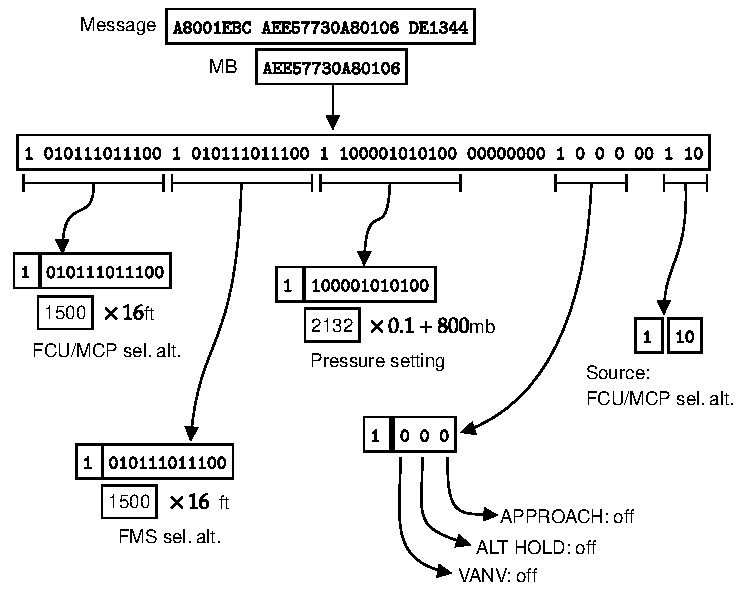
\includegraphics[scale=0.9]{figures/mode_s/bds40_example.pdf}
  \caption{BDS 4,0 decoding example}
  \label{fig:bds40_example}
\end{figure}

\begin{notebox}{Try it out}
Using pyModeS, we can decode information of BDS 4,0 messages as: 

\begin{verbatim}
import pyModeS as pms

msg = "A8001EBCAEE57730A80106DE1344"

pms.commb.selalt40fms(msg)
# 24000, FMS selected altitude (ft)

pms.commb.selalt40mcp(msg)
# 24000, MCP selected altitude (ft)

pms.commb.p40baro(msg)
# 1013.2, pressure (mb)
\end{verbatim}

\end{notebox}


\clearpage

\section{Track and turn report (BDS 5,0)}

The track and turn report is designed to provide parameters to describe aircraft turns. In this type of message, roll angle, track angle, and track rate are provided. It also includes the ground speed and true airspeed (TAS) of the aircraft.

Table \ref{tb:bds50} shows the structure of the message.

\begin{table}[ht]
\renewcommand{\arraystretch}{1.1}
\centering
\caption{Track and turn report (BDS 5,0), MB field}
\label{tb:bds50}
\begin{tabular}{|l|l|l|l|}
\hline
\textbf{FIELD} & \textbf{MSG} & \textbf{MB} & \textbf{BITS} \\ \hline
Status (for roll angle) & 33 & 1 & 1 \\ \cdashline{1-4}
Sign & 34 & 2 & 1 \\ \cdashline{1-4}
Roll angle & 35--43 & 3--11 & 9\\
~~Range: {[}-90, +90{]} degrees &&& \\
~~LSB: 45/256 degrees &&& \\ \hline
Status (for track angle) & 44 & 12 & 1 \\ \cdashline{1-4}
Sign & 45 & 13 & 1 \\ \cdashline{1-4}
True track angle & 46--55 & 14--23 & 10 \\
~~Range: {[}-180, 180{]} degrees &&& \\
~~LSB: 90/512 degrees &&& \\ \hline
Status (for ground speed) & 56 & 24 & 1 \\ \cdashline{1-4}
Ground speed & 57--66 & 25--34 & 10\\
~~Range: {[}0, 2046{]} kt &&& \\
~~LSB: 2 kt &&& \\ \hline
Status (for track angle rate) & 67 & 35 & 1 \\ \cdashline{1-4}
Sign & 68 & 36 & 1 \\ \cdashline{1-4}
Track angle rate & 69--77 & 37--45 & 9 \\
~~Range: {[}-16, 16{]} degrees/second &&& \\
~~LSB: 8/256 degrees/second &&& \\ \hline
Status (for true airspeed) & 78 & 46 & 1 \\ \cdashline{1-4}
True airspeed & 79--88 & 47--56 & 10 \\
~~Range: {[}0, 2046{]} kt &&& \\
~~LSB: 2 kt &&& \\ \hline
\end{tabular}
\end{table}

In this message, we can see three signed values, which are roll angle, track angle, and track angle rate. Two's complement coding (see section \ref{sec:two_complement}) should be used to calculate these values. 

The following Figure \ref{fig:bds50_example} shows an example of decoding a BDS 5,0 message.

\begin{figure}[ht]
  \centering
  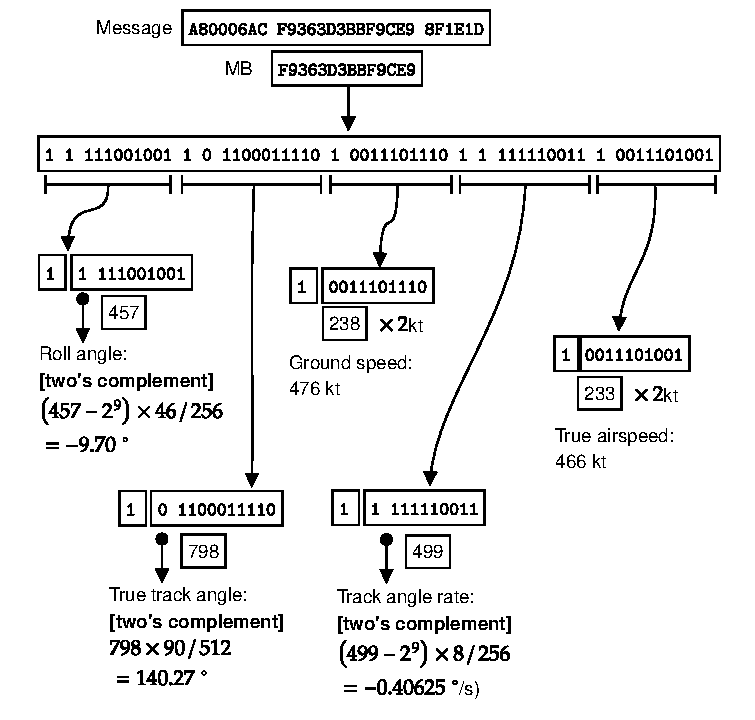
\includegraphics[scale=0.9]{figures/mode_s/bds50_example.pdf}
  \caption{BDS 5,0 decoding example}
  \label{fig:bds50_example}
\end{figure}

\begin{notebox}{Try it out}
Using pyModeS, we can decode information of BDS 5,0 messages as: 

\begin{verbatim}
import pyModeS as pms

msg = "A80006ACF9363D3BBF9CE98F1E1D"

pms.commb.roll50(msg)   # -9.7, roll angle (deg)
pms.commb.trk50(msg)    # 140.273, track angle (deg)
pms.commb.rtrk50(msg)   # -0.406, track angle rate (deg/s)
pms.commb.gs50(msg)     # 476, ground speed (kt)
pms.commb.tas50(msg)    # 466, TAS (kt)

\end{verbatim}

\end{notebox}


\clearpage

\section{Heading and speed report (BDS 6,0)}

The heading and speed report is designed to downlink various airspeed and vertical rate to air traffic controllers. In this type of message, indicated airspeed (IAS), Mach number, barometric altitude rate, inertial vertical velocity, and the magnetic heading of the aircraft are provided.

Table \ref{tb:bds60} shows the structure of the message.


\begin{table}[ht]
\renewcommand{\arraystretch}{1.1}
\centering
\caption{Heading and speed report (BDS 6,0), MB field}
\label{tb:bds60}
\begin{tabular}{|l|l|l|l|}
\hline
\textbf{FIELD} & \textbf{MSG} & \textbf{MB} & \textbf{BITS} \\ \hline
Status (for magnetic heading) & 33 & 1 & 1 \\ \cdashline{1-4}
Sign & 34 & 2 & 1 \\ \cdashline{1-4}
Magnetic heading & 35--44 & 3--12 & 10\\
Range: {[}-180, +180{]} degrees &&& \\
LSB: 90/512 degrees &&& \\ \hline
Status (for indicated airspeed) & 45 & 13 & 1 \\ \cdashline{1-4}
Indicated airspeed  & 46--55 & 14--23 & 10\\
Range: {[}0, 1023{]} kt &&& \\
LSB: 1 kt &&& \\ \hline
Status (for Mach number) & 56 & 24 & 1 \\ \cdashline{1-4}
Mach number & 57--66 & 25--34 & 10\\
Range: {[}0, 4.092{]} &&&\\
LSB: 0.004 &&& \\ \hline
Status (for barometric altitude rate) & 67 & 35 & 1 \\ \cdashline{1-4}
Sign & 68 & 36 & 1 \\ \cdashline{1-4}
Barometric altitude rate  & 69--77 & 37--45 & 9 \\
Range: {[}-16384, +16352{]} ft/min &&& \\
LSB: 32 ft/min &&& \\ \hline
Status (for inertial vertical velocity) & 78 & 46 & 1 \\ \cdashline{1-4}
Sign & 79 & 47 & 1 \\ \cdashline{1-4}
Inertial vertical velocity & 80--88 & 48--56 & 9\\
Range: {[}-16384, +16352{]} ft/min &&& \\
LSB: 32 ft/min &&& \\ \hline
\end{tabular}
\end{table}

In this message, we can see a few signed values, such as heading and two vertical rates. Two's complement coding (see section \ref{sec:two_complement}) should be used to calculate these values.

The magnetic heading is the aircraft's heading with respect to the magnetic North, which can be different from the true north (for example, used for the track angle from ADS-B and BDS 5,0). Often an aircraft obtains the magnetic heading by adding its true North heading with the magnetic declination from a world magnetic model, such as \cite{chulliat2015}. It is worth noting that the true North heading is not necessarily the same as the track angle due to the influence of wind.

In the heading and speed report, two different kinds of vertical rates are reported. Barometric altitude rates are only derived from barometer measurements. Since the source data from air data system is not filtered, significant noise is contained in these values. In contrast, inertial vertical velocities are values provided by navigational equipment from different sources including the flight management computer. According to \cite{icao9688}, data sources with different levels of priorities are defined for these two values, which are listed in Table \ref{tb:vertical_rate_source}.

\begin{table}[ht]
\footnotesize
\centering
\caption{Data sources for two vertical rates in heading and speed report}
\label{tb:vertical_rate_source}
\begin{tabular}{|l|l|}
\hline
\textbf{Parameter} & \textbf{Input Data Source Priorities} \\ \hline
Barometric altitude rate & 1. Air Data System\\ 
& 2. Inertial Reference System/Flight Management System \\ \hline
Inertial vertical velocity & 1. Flight Management Computer / GNSS integrated\\ 
& 2. Flight Management Computer (General)\\
& 3. Inertial Reference System/Flight Management System \\ \hline
\end{tabular}
\end{table}


Figure \ref{fig:bds60_example} illustrates an example on how to decode a BDS 6,0 message.

\begin{figure}[ht]
  \centering
  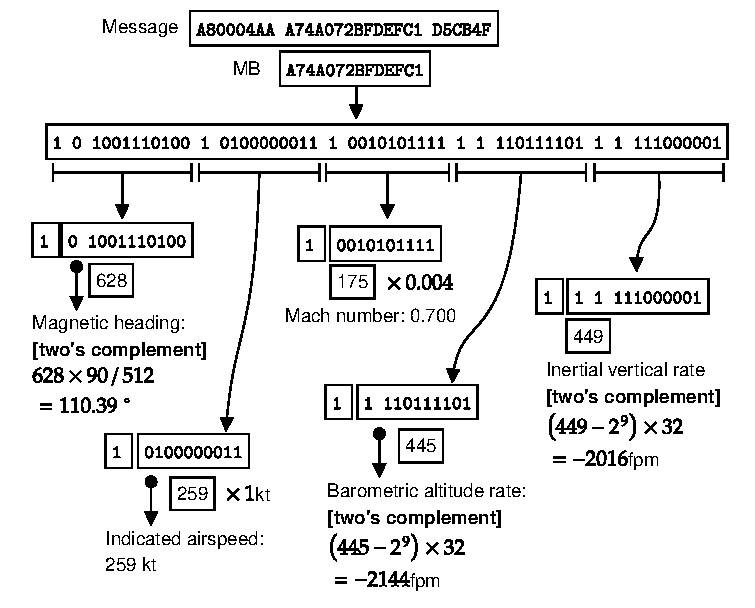
\includegraphics[scale=0.9]{figures/mode_s/bds60_example.pdf}
  \caption{BDS 6,0 decoding example}
  \label{fig:bds60_example}
\end{figure}

\begin{notebox}{Try it out}
Using pyModeS, we can decode information of BDS 6,0 messages as: 

\begin{verbatim}
import pyModeS as pms

msg = "A80004AAA74A072BFDEFC1D5CB4F"

pms.commb.hdg60(msg)      # 110.391, heading (deg)
pms.commb.ias60(msg)      # 259, ISA (kt)
pms.commb.mach60(msg)     # 0.7, Mach (-)
pms.commb.vr60baro(msg)   # -2144, baro vertical rate (ft/min)
pms.commb.vr60ins(msg)    # -2016, INS vertical rate (ft/min)
\end{verbatim}

\end{notebox}

\chapter{Mode~S meteorological services}

In the current Mode~S design, two message formats are used for aircraft to communicate meteorological conditions. These messages are meteorological routine air report (MRAR) and meteorological hazard report (MHR). In this chapter, we focus on explaining the information contained in these two types of messages.

\section{Meteorological routine air report (BDS 4,4)}

In MRAR messages, information on wind, air temperature, pressure, and humidity is transmitted. The structure of the message is shown in Table \ref{tb:bds44}.


\begin{table}[ht]
\renewcommand{\arraystretch}{1.1}
\centering
\caption{Meteorological routine air report (BDS 4,4), MB field}
\label{tb:bds44}
\begin{tabular}{|l|l|l|l|}
\hline
\textbf{FIELD} & \textbf{MSG} & \textbf{MB} & \textbf{BITS} \\ \hline
Figure of merit / source & 33-36 & 1-4 & 4 \\ \hline
Status (for wind) & 37 & 5 & 1 \\ \cdashline{1-1}
\begin{tabular}[c]{@{}l@{}}Wind speed\\ ~~\footnotesize Range: {[}0, 511{]} knots\\ ~~\footnotesize LSB: 1 knots\end{tabular} & 38-46 & 6-14 & 9 \\ \cdashline{1-1}
\begin{tabular}[c]{@{}l@{}}Wind direction\\ ~~\footnotesize Range: {[}0, 360{]} degrees\\ ~~\footnotesize LSB: 180/256 degrees\end{tabular} & 47-55 & 15-23 & 9 \\ \hline
Sign (for temperature) & 56 & 24 & 1 \\ \cdashline{1-1}
\begin{tabular}[c]{@{}l@{}}Static air temperature\\ ~~\footnotesize Range: {[}-128, +128{]} $^\circ$C\\ ~~\footnotesize LSB: 0.25 $^\circ$C \end{tabular} & 57-66 & 25-34 & 10 \\ \hline
Status (for pressure) & 67 & 35 & 1 \\ \cdashline{1-1}
\begin{tabular}[c]{@{}l@{}}Average static pressure\\ ~~\footnotesize Range: {[}0, 2048{]} hPa\\ ~~\footnotesize LSB: 1 hPa\end{tabular} & 68-78 & 36-46 & 11 \\ \hline
Status (for turbulence) & 79 & 47 & 1 \\ \cdashline{1-1}
Turbulence & 80-81 & 48-49 & 2 \\ \hline
Status (for humidity) & 82 & 50 & 1 \\ \cdashline{1-1}
\begin{tabular}[c]{@{}l@{}}Humidity\\ ~~\footnotesize Range: {[}0\%, 100\%{]} \\ ~~\footnotesize LSB: 100/64 \%\end{tabular} & 83-88 & 51-56 & 6 \\ \hline
\end{tabular}
\end{table}

The first field of the message defined the figure of merit (FOM) / source of the information. The values indicate the following:
\begin{itemize}
    \item 0: Invalid
    \item 1: Intertial system (INS)
    \item 2: Global Navigation Satellite System (GNSS)
    \item 3: Distance measuring equipment-based navigation (DME/DME)
    \item 4: Very High Frequency omnidirectional range / distance measuring equipment-based navigation (VOR/DME)
    \item 5-15: Reserved
\end{itemize}

For static air temperature, the encoded value can be negative. Hence, two's complement coding (see section \ref{sec:two_complement}) is used for decoding. The actual maximum range of temperature is from -80 $^\circ$C to +60 $^\circ$C.

It is also worth pointing out a discrepancy in the design. The temperature is encoded using 10 bits, where the least significant bit value should have been 0.125$^\circ$. However, according to the official document \cite{icao9871v1}, the LSB value is 0.25$^\circ$. ICAO has planned to update this to 0.125$^\circ$ in the future. Most current implementations still use 0.25$^\circ$. 

In Figure \ref{fig:bds44_example}, the decoding of an MRAR example message is shown.

\begin{figure}[ht]
    \centering
    

\tikzset{every picture/.style={line width=0.75pt}} %set default line width to 0.75pt        

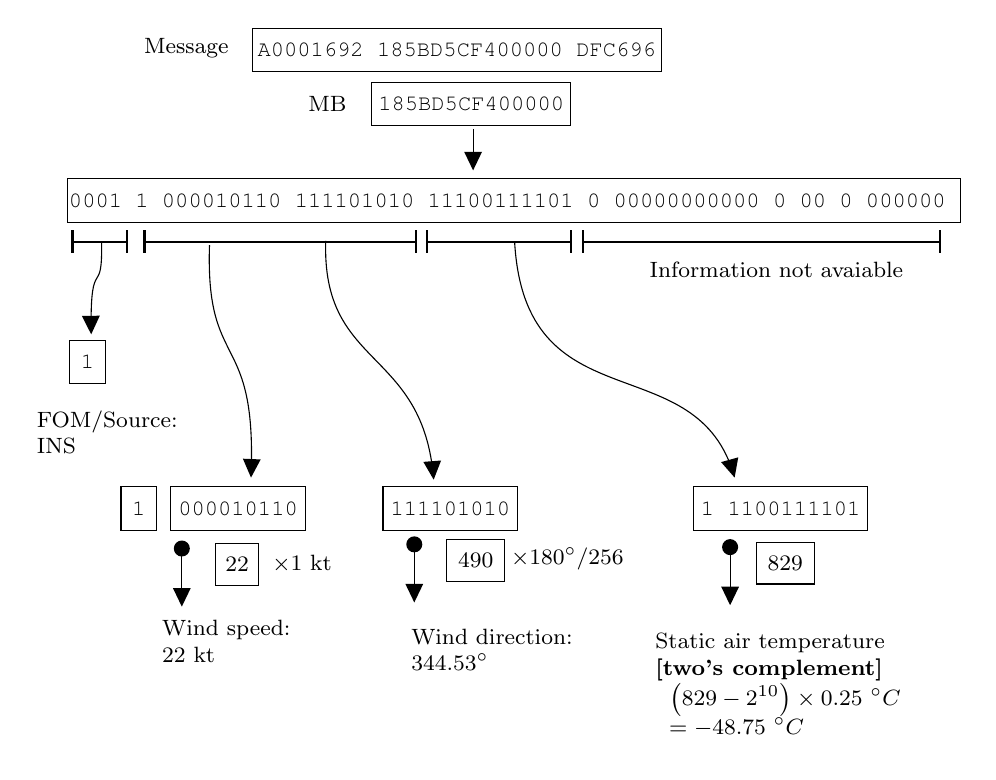
\begin{tikzpicture}[x=0.75pt,y=0.75pt,yscale=-1,xscale=1]
%uncomment if require: \path (0,402); %set diagram left start at 0, and has height of 402

%Curve Lines [id:da4469785122246488] 
\draw    (53,117.33) .. controls (53.57,145.77) and (47.64,122.56) .. (47.96,159.07) ;
\draw [shift={(48,162)}, rotate = 269.06] [fill={rgb, 255:red, 0; green, 0; blue, 0 }  ][line width=0.08]  [draw opacity=0] (8.93,-4.29) -- (0,0) -- (8.93,4.29) -- cycle    ;
%Curve Lines [id:da048475740519535515] 
\draw    (105,119) .. controls (103.02,180.38) and (127.5,159.43) .. (125.08,228.87) ;
\draw [shift={(125,231)}, rotate = 272.39] [fill={rgb, 255:red, 0; green, 0; blue, 0 }  ][line width=0.08]  [draw opacity=0] (8.93,-4.29) -- (0,0) -- (8.93,4.29) -- cycle    ;
%Straight Lines [id:da5412152919437994] 
\draw [line width=0.75]    (209.67,117.33) -- (279,117.33) ;
\draw [shift={(279,117.33)}, rotate = 180] [color={rgb, 255:red, 0; green, 0; blue, 0 }  ][line width=0.75]    (0,5.59) -- (0,-5.59)   ;
\draw [shift={(209.67,117.33)}, rotate = 180] [color={rgb, 255:red, 0; green, 0; blue, 0 }  ][line width=0.75]    (0,5.59) -- (0,-5.59)   ;
%Straight Lines [id:da12370443285273769] 
\draw [line width=0.75]    (73.67,117.33) -- (204.67,117.33) ;
\draw [shift={(204.67,117.33)}, rotate = 180] [color={rgb, 255:red, 0; green, 0; blue, 0 }  ][line width=0.75]    (0,5.59) -- (0,-5.59)   ;
\draw [shift={(73.67,117.33)}, rotate = 180] [color={rgb, 255:red, 0; green, 0; blue, 0 }  ][line width=0.75]    (0,5.59) -- (0,-5.59)   ;
%Straight Lines [id:da4904702793159954] 
\draw [line width=0.75]    (39,117.33) -- (65.33,117.33) ;
\draw [shift={(65.33,117.33)}, rotate = 180] [color={rgb, 255:red, 0; green, 0; blue, 0 }  ][line width=0.75]    (0,5.59) -- (0,-5.59)   ;
\draw [shift={(39,117.33)}, rotate = 180] [color={rgb, 255:red, 0; green, 0; blue, 0 }  ][line width=0.75]    (0,5.59) -- (0,-5.59)   ;
%Straight Lines [id:da3760076772420655] 
\draw [line width=0.75]    (285,117.33) -- (457,117.33) ;
\draw [shift={(457,117.33)}, rotate = 180] [color={rgb, 255:red, 0; green, 0; blue, 0 }  ][line width=0.75]    (0,5.59) -- (0,-5.59)   ;
\draw [shift={(285,117.33)}, rotate = 180] [color={rgb, 255:red, 0; green, 0; blue, 0 }  ][line width=0.75]    (0,5.59) -- (0,-5.59)   ;
%Curve Lines [id:da970561260907983] 
\draw    (252,117.33) .. controls (256.93,205.66) and (337.53,167.2) .. (357.15,228.15) ;
\draw [shift={(358,231)}, rotate = 254.51999999999998] [fill={rgb, 255:red, 0; green, 0; blue, 0 }  ][line width=0.08]  [draw opacity=0] (8.93,-4.29) -- (0,0) -- (8.93,4.29) -- cycle    ;
%Straight Lines [id:da1281375538700964] 
\draw    (232,63) -- (232,80) ;
\draw [shift={(232,83)}, rotate = 270] [fill={rgb, 255:red, 0; green, 0; blue, 0 }  ][line width=0.08]  [draw opacity=0] (8.93,-4.29) -- (0,0) -- (8.93,4.29) -- cycle    ;
%Straight Lines [id:da869507612596206] 
\draw    (91.67,265.17) -- (91.67,290.17) ;
\draw [shift={(91.67,293.17)}, rotate = 270] [fill={rgb, 255:red, 0; green, 0; blue, 0 }  ][line width=0.08]  [draw opacity=0] (8.93,-4.29) -- (0,0) -- (8.93,4.29) -- cycle    ;
\draw [shift={(91.67,265.17)}, rotate = 90] [color={rgb, 255:red, 0; green, 0; blue, 0 }  ][fill={rgb, 255:red, 0; green, 0; blue, 0 }  ][line width=0.75]      (0, 0) circle [x radius= 3.35, y radius= 3.35]   ;
%Straight Lines [id:da8277360726929222] 
\draw    (355.83,264.5) -- (355.83,289.5) ;
\draw [shift={(355.83,292.5)}, rotate = 270] [fill={rgb, 255:red, 0; green, 0; blue, 0 }  ][line width=0.08]  [draw opacity=0] (8.93,-4.29) -- (0,0) -- (8.93,4.29) -- cycle    ;
\draw [shift={(355.83,264.5)}, rotate = 90] [color={rgb, 255:red, 0; green, 0; blue, 0 }  ][fill={rgb, 255:red, 0; green, 0; blue, 0 }  ][line width=0.75]      (0, 0) circle [x radius= 3.35, y radius= 3.35]   ;
%Curve Lines [id:da2502337031348296] 
\draw    (161,117) .. controls (159.03,178.07) and (206.54,168.31) .. (212.75,229.17) ;
\draw [shift={(213,232)}, rotate = 265.53] [fill={rgb, 255:red, 0; green, 0; blue, 0 }  ][line width=0.08]  [draw opacity=0] (8.93,-4.29) -- (0,0) -- (8.93,4.29) -- cycle    ;
%Straight Lines [id:da9802254187880033] 
\draw    (203.67,263.17) -- (203.67,288.17) ;
\draw [shift={(203.67,291.17)}, rotate = 270] [fill={rgb, 255:red, 0; green, 0; blue, 0 }  ][line width=0.08]  [draw opacity=0] (8.93,-4.29) -- (0,0) -- (8.93,4.29) -- cycle    ;
\draw [shift={(203.67,263.17)}, rotate = 90] [color={rgb, 255:red, 0; green, 0; blue, 0 }  ][fill={rgb, 255:red, 0; green, 0; blue, 0 }  ][line width=0.75]      (0, 0) circle [x radius= 3.35, y radius= 3.35]   ;

% Text Node
\draw    (125.63,14.5) -- (322.63,14.5) -- (322.63,35.5) -- (125.63,35.5) -- cycle  ;
\draw (224.13,25) node  [font=\footnotesize] [align=left] {{\fontfamily{pcr}\selectfont A0001692 185BD5CF400000 DFC696}};
% Text Node
\draw (161.88,51) node  [font=\footnotesize] [align=left] {MB};
% Text Node
\draw    (36.7,87) -- (466.7,87) -- (466.7,108) -- (36.7,108) -- cycle  ;
\draw (251.7,97.5) node  [font=\footnotesize] [align=left] {{\fontfamily{pcr}\selectfont 0001 1 000010110 111101010 11100111101 0 00000000000 0 00 0 000000 }};
% Text Node
\draw    (183.13,40.5) -- (279.13,40.5) -- (279.13,61.5) -- (183.13,61.5) -- cycle  ;
\draw (231.13,51) node  [font=\footnotesize] [align=left] {{\fontfamily{pcr}\selectfont 185BD5CF400000}};
% Text Node
\draw    (37.76,164.75) -- (54.76,164.75) -- (54.76,185.75) -- (37.76,185.75) -- cycle  ;
\draw (46.26,175.25) node  [font=\footnotesize] [align=left] {{\fontfamily{pcr}\selectfont 1}};
% Text Node
\draw    (62.38,235.33) -- (79.38,235.33) -- (79.38,256.33) -- (62.38,256.33) -- cycle  ;
\draw (70.88,245.83) node  [font=\footnotesize] [align=left] {{\fontfamily{pcr}\selectfont 1}};
% Text Node
\draw    (86.26,235.33) -- (151.26,235.33) -- (151.26,256.33) -- (86.26,256.33) -- cycle  ;
\draw (118.76,245.83) node  [font=\footnotesize] [align=left] {{\fontfamily{pcr}\selectfont 000010110}};
% Text Node
\draw    (107.76,262.92) -- (128.76,262.92) -- (128.76,282.92) -- (107.76,282.92) -- cycle  ;
\draw (118.26,272.92) node  [font=\footnotesize] [align=left] {22};
% Text Node
\draw (93.82,24) node  [font=\footnotesize] [align=left] {Message};
% Text Node
\draw    (338.2,235.33) -- (422.2,235.33) -- (422.2,256.33) -- (338.2,256.33) -- cycle  ;
\draw (380.2,245.83) node  [font=\footnotesize] [align=left] {{\fontfamily{pcr}\selectfont 1 1100111101}};
% Text Node
\draw (55.76,209.17) node  [font=\footnotesize] [align=left] {FOM/Source:\\INS};
% Text Node
\draw (113.09,309.83) node  [font=\footnotesize] [align=left] {Wind speed:\\22 kt};
% Text Node
\draw    (368.42,262.25) -- (396.42,262.25) -- (396.42,282.25) -- (368.42,282.25) -- cycle  ;
\draw (382.42,272.25) node  [font=\footnotesize] [align=left] {829};
% Text Node
\draw (382.26,332.5) node  [font=\footnotesize] [align=left] {Static air temperature\\\textbf{[two's complement]}\\$\displaystyle  \begin{array}{{>{\displaystyle}l}}
\left( 829-2^{10}\right) \times 0.25\ ^{\circ } C\\
=-48.75\ ^{\circ } C
\end{array}$};
% Text Node
\draw (134,272.75) node [anchor=west] [inner sep=0.75pt]  [font=\footnotesize] [align=left] {$\displaystyle \times 1$ kt};
% Text Node
\draw    (188.59,235.33) -- (253.59,235.33) -- (253.59,256.33) -- (188.59,256.33) -- cycle  ;
\draw (221.09,245.83) node  [font=\footnotesize] [align=left] {{\fontfamily{pcr}\selectfont 111101010}};
% Text Node
\draw    (219.26,260.92) -- (247.26,260.92) -- (247.26,280.92) -- (219.26,280.92) -- cycle  ;
\draw (233.26,270.92) node  [font=\footnotesize] [align=left] {490};
% Text Node
\draw (241.09,313.83) node  [font=\footnotesize] [align=left] {Wind direction:\\344.53$\displaystyle ^{\circ }$};
% Text Node
\draw (249,270.08) node [anchor=west] [inner sep=0.75pt]  [font=\footnotesize] [align=left] {$\displaystyle \times 180^{\circ } /256${\fontfamily{pcr}\selectfont  }};
% Text Node
\draw (378.09,130.83) node  [font=\footnotesize] [align=left] {Information not avaiable};


\end{tikzpicture}
    \caption{Meteorological routine air report (BDS 4,4) decoding example}
    \label{fig:bds44_example}
  \end{figure}
  
\begin{notebox}{Try it out}
Using \texttt{pyModeS}, we can decode information of BDS 4,4 messages as: 

\begin{verbatim}
import pyModeS as pms

msg = "A0001692185BD5CF400000DFC696"

wind = pms.commb.wind44(msg)
temperature = pms.commb.temp44(msg)
pressure = pms.commb.p44(msg)
humidity = pms.commb.hum44(msg)
\end{verbatim}

\end{notebox}

\clearpage
\section{Meteorological hazard report (BDS 4,5)}

In MHR messages, different hazard condition levels are reported, such as turbulence, wind shear, microburst, icing, and wake vortex. It also includes temperature, pressure, and radio height. In Table \ref{tb:bds45}, the structure of the MHR message is shown.

It is worth noting that during real flights, MHR messages are much rarer than MARA messages. Whenever they are available, most of the messages only contain temperature information.

\begin{table}[ht]
\renewcommand{\arraystretch}{1.1}
\centering
\caption{Meteorological harzard report (BDS 4,5), MB field}
\label{tb:bds45}
\begin{tabular}{|l|l|l|l|}
\hline
\textbf{FIELD} & \textbf{MSG} & \textbf{MB} & \textbf{BITS} \\ \hline
Status (for turbulence) & 33 & 1 & 1 \\ \cdashline{1-1}
Turbulence & 34-35 & 2-3 & 2 \\ \hline
Status (for wind shear) & 36 & 4 & 1 \\ \cdashline{1-1}
Wind shear & 37-38 & 5-6 & 2 \\ \hline
Status (for microburst) & 39 & 7 & 1 \\ \cdashline{1-1}
Microburst & 40-41 & 8-9 & 2 \\ \hline
Status (for icing) & 42 & 10 & 1 \\ \cdashline{1-1}
Icing & 43-44 & 11-12 & 2 \\ \hline
Status (for wake vortex) & 45 & 13 & 1 \\ \cdashline{1-1}
Wake vortex & 46-47 & 14-15 & 2 \\ \hline
Status (for temperature) & 48 & 16 & 1 \\ \cdashline{1-1}
Sign (for temperature) & 49 & 17 & 1 \\ \cdashline{1-1}
\begin{tabular}[c]{@{}l@{}} Static air temperature\\ ~~\footnotesize Range: {[}-128, +128{]} $^\circ$C\\ ~~\footnotesize LSB: 0.25 $^\circ$C\end{tabular} & 50-58 & 18-26 & 9 \\ \hline
Status (for pressure) & 59 & 27 & 1 \\ \cdashline{1-1}
\begin{tabular}[c]{@{}l@{}}Average static pressure\\ ~~\footnotesize Range: {[}0, 2048{]} hPa\\ ~~\footnotesize LSB: 1 hPa\end{tabular} & 60-70 & 28-38 & 11 \\ \hline
Status (for height) & 71 & 39 & 1 \\ \cdashline{1-1}
\begin{tabular}[c]{@{}l@{}}Radio height\\ ~~\footnotesize Range: {[}0, 65 528{]} ft\\ ~~\footnotesize LSB: 16 ft\end{tabular} & 72-83 & 40-51 & 12 \\ \hline
Reserved & 84-88 & 52-56 & 5 \\ \hline
\end{tabular}
\end{table}

The levels for turbulence, wind shear, microburst, icing, and wake vortex are encoded as follows:
\begin{itemize}
  \item \texttt{00}: NIL
  \item \texttt{01}: LIGHT
  \item \texttt{10}: MODERATE
  \item \texttt{11}: SEVERE
\end{itemize}

As is the case for MRAR messages, the actual range of the temperature is from -80 $^\circ$C to +60 $^\circ$C, and it is encoded using the two's complement coding.

In Figure \ref{fig:bds45_example}, the decoding of an example message is shown. Note that in this example, only the air temperature information is included. None of the hazard conditions is reported.

\begin{figure}[ht]
  \centering
  

\tikzset{every picture/.style={line width=0.75pt}} %set default line width to 0.75pt        

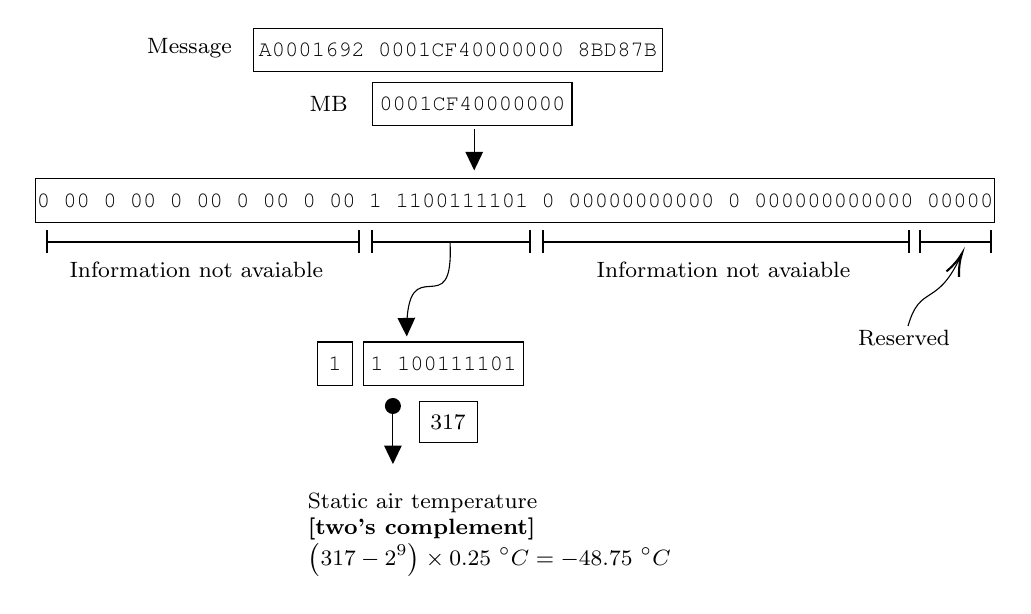
\begin{tikzpicture}[x=0.75pt,y=0.75pt,yscale=-1,xscale=1]
%uncomment if require: \path (0,368); %set diagram left start at 0, and has height of 368

%Straight Lines [id:da4065588661974868] 
\draw [line width=0.75]    (182.67,117.33) -- (259,117.33) ;
\draw [shift={(259,117.33)}, rotate = 180] [color={rgb, 255:red, 0; green, 0; blue, 0 }  ][line width=0.75]    (0,5.59) -- (0,-5.59)   ;
\draw [shift={(182.67,117.33)}, rotate = 180] [color={rgb, 255:red, 0; green, 0; blue, 0 }  ][line width=0.75]    (0,5.59) -- (0,-5.59)   ;
%Straight Lines [id:da8606101743392234] 
\draw [line width=0.75]    (265,117.33) -- (441.5,117.33) ;
\draw [shift={(441.5,117.33)}, rotate = 180] [color={rgb, 255:red, 0; green, 0; blue, 0 }  ][line width=0.75]    (0,5.59) -- (0,-5.59)   ;
\draw [shift={(265,117.33)}, rotate = 180] [color={rgb, 255:red, 0; green, 0; blue, 0 }  ][line width=0.75]    (0,5.59) -- (0,-5.59)   ;
%Curve Lines [id:da10322788127976112] 
\draw    (220.33,117.33) .. controls (222.46,159.15) and (199.45,118.69) .. (199.47,160.35) ;
\draw [shift={(199.5,163)}, rotate = 268.75] [fill={rgb, 255:red, 0; green, 0; blue, 0 }  ][line width=0.08]  [draw opacity=0] (8.93,-4.29) -- (0,0) -- (8.93,4.29) -- cycle    ;
%Straight Lines [id:da8466832782097071] 
\draw    (232,63) -- (232,80) ;
\draw [shift={(232,83)}, rotate = 270] [fill={rgb, 255:red, 0; green, 0; blue, 0 }  ][line width=0.08]  [draw opacity=0] (8.93,-4.29) -- (0,0) -- (8.93,4.29) -- cycle    ;
%Straight Lines [id:da4977418628626593] 
\draw    (192.83,196.5) -- (192.83,221.5) ;
\draw [shift={(192.83,224.5)}, rotate = 270] [fill={rgb, 255:red, 0; green, 0; blue, 0 }  ][line width=0.08]  [draw opacity=0] (8.93,-4.29) -- (0,0) -- (8.93,4.29) -- cycle    ;
\draw [shift={(192.83,196.5)}, rotate = 90] [color={rgb, 255:red, 0; green, 0; blue, 0 }  ][fill={rgb, 255:red, 0; green, 0; blue, 0 }  ][line width=0.75]      (0, 0) circle [x radius= 3.35, y radius= 3.35]   ;
%Straight Lines [id:da5955016490623266] 
\draw [line width=0.75]    (26,117.33) -- (176.5,117.33) ;
\draw [shift={(176.5,117.33)}, rotate = 180] [color={rgb, 255:red, 0; green, 0; blue, 0 }  ][line width=0.75]    (0,5.59) -- (0,-5.59)   ;
\draw [shift={(26,117.33)}, rotate = 180] [color={rgb, 255:red, 0; green, 0; blue, 0 }  ][line width=0.75]    (0,5.59) -- (0,-5.59)   ;
%Straight Lines [id:da5052935437984565] 
\draw [line width=0.75]    (446.67,117.33) -- (481,117.33) ;
\draw [shift={(481,117.33)}, rotate = 180] [color={rgb, 255:red, 0; green, 0; blue, 0 }  ][line width=0.75]    (0,5.59) -- (0,-5.59)   ;
\draw [shift={(446.67,117.33)}, rotate = 180] [color={rgb, 255:red, 0; green, 0; blue, 0 }  ][line width=0.75]    (0,5.59) -- (0,-5.59)   ;
%Curve Lines [id:da0284439343230396] 
\draw    (441,158) .. controls (446.88,137.42) and (454.68,149.49) .. (466.28,124.57) ;
\draw [shift={(467,123)}, rotate = 473.96] [color={rgb, 255:red, 0; green, 0; blue, 0 }  ][line width=0.75]    (10.93,-3.29) .. controls (6.95,-1.4) and (3.31,-0.3) .. (0,0) .. controls (3.31,0.3) and (6.95,1.4) .. (10.93,3.29)   ;

% Text Node
\draw    (125.63,14.5) -- (322.63,14.5) -- (322.63,35.5) -- (125.63,35.5) -- cycle  ;
\draw (224.13,25) node  [font=\footnotesize] [align=left] {{\fontfamily{pcr}\selectfont A0001692 0001CF40000000 8BD87B}};
% Text Node
\draw (161.88,51) node  [font=\footnotesize] [align=left] {MB};
% Text Node
\draw    (20.7,87) -- (482.7,87) -- (482.7,108) -- (20.7,108) -- cycle  ;
\draw (251.7,97.5) node  [font=\footnotesize] [align=left] {{\fontfamily{pcr}\selectfont 0 00 0 00 0 00 0 00 0 00 1 1100111101 0 00000000000 0 000000000000 00000}};
% Text Node
\draw    (183.13,40.5) -- (279.13,40.5) -- (279.13,61.5) -- (183.13,61.5) -- cycle  ;
\draw (231.13,51) node  [font=\footnotesize] [align=left] {{\fontfamily{pcr}\selectfont 0001CF40000000}};
% Text Node
\draw (94.82,24) node  [font=\footnotesize] [align=left] {Message};
% Text Node
\draw    (156.38,165.67) -- (173.38,165.67) -- (173.38,186.67) -- (156.38,186.67) -- cycle  ;
\draw (164.88,176.17) node  [font=\footnotesize] [align=left] {{\fontfamily{pcr}\selectfont 1}};
% Text Node
\draw    (178.7,165.67) -- (255.7,165.67) -- (255.7,186.67) -- (178.7,186.67) -- cycle  ;
\draw (217.2,176.17) node  [font=\footnotesize] [align=left] {{\fontfamily{pcr}\selectfont 1 100111101}};
% Text Node
\draw    (205.42,194.25) -- (233.42,194.25) -- (233.42,214.25) -- (205.42,214.25) -- cycle  ;
\draw (219.42,204.25) node  [font=\footnotesize] [align=left] {317};
% Text Node
\draw (239.26,258.5) node  [font=\footnotesize] [align=left] {Static air temperature\\\textbf{[two's complement]}\\$\displaystyle \left( 317-2^{9}\right) \times 0.25\ ^{\circ } C=-48.75\ ^{\circ } C$};
% Text Node
\draw (352.09,130.83) node  [font=\footnotesize] [align=left] {Information not avaiable};
% Text Node
\draw (98.09,130.83) node  [font=\footnotesize] [align=left] {Information not avaiable};
% Text Node
\draw (439.09,163.83) node  [font=\footnotesize] [align=left] {Reserved};


\end{tikzpicture}

  \caption{Meteorological harzard report (BDS 4,5) decoding example}
  \label{fig:bds45_example}
\end{figure}


\begin{notebox}{Note}
The availability of BDS 4,4 messages is quite low. Very few aircraft's transponders have these capabilities enabled. BDS 4,5 message is even rarer. When a message is transmitted, it is very common that information in many fields are not available.
\end{notebox}


\chapter{Inferencing of BDS codes}

In chapter \ref{chap:comm-b}, we discussed the basic structure and protocols of Mode~S Comm-B messages. Each message type is identified by an 8-bit Comm-B Data Selector (BDS) code, which is only transmitted in the uplink message but not included in the downlink message. As third parties observing the replies to Mode~S surveillance interrogations, we must first determine the BDS code before decoding the content of any Comm-B messages. 


\section{BDS codes identification logics}

Each Mode~S message has a predefined structure and variables. For almost all common Comm-B message types, there are rules for certain bits. For example, these bits are:
\begin{itemize}
    \item Reserved bits: Those are bits in the different message types that are reserved for future use. They all have to be zeros. If any of the bits is not zero, the possibility of a certain BDS code should be ruled out.
    \item Status bits: Some fields in Comm-B messages have their corresponding status bits. When a status bit is set to zero, all bits in the field must be zero. If the field contains non zero bits, the possibility of a certain BDS code can be ruled out.
    \item Value rules: Different fields in the messages also have different physical ranges. For example, the Mach number in BDS 6,0 should not be higher than 1, and the temperature value in BDS 4,4 should be between -80$^\circ C$ and 60$^\circ C$. These constants can also be used to exclude certain BDS codes.
\end{itemize}


In Tables \ref{tb:bds_rule_els}, \ref{tb:bds_rule_ehs}, and \ref{tb:bds_rule_mrar}, the rules for identifiying different types of ELS, EHS, and meteorlogical messages are shown.


\begin{table}
\centering
\small
\caption{Heuristic indenfication logic for ELS}
\label{tb:bds_rule_els}
\begin{tabular}{|l|l|l|l|}
\hline
\textbf{BDS} & \textbf{MB bits} & \textbf{Parameter} & \textbf{Rules} \\ \hline \hline
\multirow{2}{*}{1,0} & 1-8 & BDS code & Equal to \texttt{0001 0000}  \\ \cline{2-4} 
 & 10-14 & Reserved & All zeros \\ \hline \hline
\multirow{2}{*}{1,7} & 7 & BDS 2,0 enabled & Equal to \texttt{1} \\ \cline{2-4} 
 & 29-56 & Reserved & All zeros \\ \hline \hline
\multirow{2}{*}{2,0} & 1-8 & BDS code & Equal to \texttt{0010 0000} \\ \cline{2-4} 
 & 9-56 & Callsign & Only contains 0-9, A-Z, or space \\ \hline \hline
\multirow{3}{*}{3,0} & 1-8 & BDS code & Equal to \texttt{0011 0000} \\ \cline{2-4} 
 & 29-30 & Threat type & Not equal to \texttt{11} \\ \cline{2-4} 
 & 16-22 & ACAS &  less than 48 \\ \hline

\end{tabular}
\end{table}



\begin{table}
\footnotesize
\centering
\small
\caption{Heuristic indenfication logic for EHS}
\label{tb:bds_rule_ehs}
\begin{tabular}{|l|l|l|l|}
\hline
\textbf{BDS} & \textbf{MB bits} & \textbf{Parameter} & \textbf{Rules} \\ \hline \hline
\multirow{5}{*}{4,0} & 1 : 2-13 & MCP/FCU selected altitude & Status consistant \\ \cline{2-4} 
& 14 : 15-26 & FMS selected altitude & Status consistant \\ \cline{2-4} 
& 27 : 28-39 & Barometric pressure & Status consistant \\ \cline{2-4} 
& 40 - 47 & Reserved & All zeros \\ \cline{2-4} 
& 52 - 53 & Reserved & All zeros \\ \hline \hline
\multirow{5}{*}{5,0} & 1 : 2-11 & Roll angle & \makecell*{Status consistant \\ Between -50 and 50 degre} \\ \cline{2-4} 
& 12 : 13-23 & True track angle & Status consistant \\ \cline{2-4} 
& 24 : 25-34 & Ground speed & \makecell*{Status consistant \\ Between 0 and 600 kt} \\ \cline{2-4} 
& 35 : 36-45 & Track angle rate & Status consistant \\ \cline{2-4} 
& 45 : 46-56 & True airspeed & \makecell*{Status consistant \\ Between 0 and 500 kt} \\ \hline \hline
\multirow{5}{*}{6,0} & 1 : 2-12 & Magnetic heading & Status consistant \\ \cline{2-4} 
& 13 : 14-23 & Indicated airspeed & \makecell*{Status consistant \\ Between 0 and 500 kt} \\ \cline{2-4} 
& 24 : 25-34 & Mach number & \makecell*{Status consistant \\ Between 0 and 1}\\ \cline{2-4} 
& 35 : 36-45 & Barometric vertical rate & \makecell*{Status consistant \\ Between -6000 and 6000 fpm} \\ \cline{2-4} 
& 46 : 47-56 & Inertial vertical rate & \makecell*{Status consistant \\ Between -6000 and 6000 fpm} \\ \hline
\end{tabular}
\end{table}


\begin{table}
\footnotesize
\centering
\small
\caption{Heuristic indenfication logic for MRAR and MHR}
\label{tb:bds_rule_mrar}
\begin{tabular}{|l|l|l|l|}
\hline
\textbf{BDS} & \textbf{MB bits} & \textbf{Parameter} & \textbf{Rules} \\ \hline \hline
\multirow{3}{*}{4,4} & 1-4 & FOM & Less than 5 \\ \cline{2-4} 
& 5 : 6-23 & Wind speed / direction & \makecell*{Status consistant \\ speed less than 250 kt} \\ \cline{2-4} 
& 24-34 & Static air temperature & Between -80 and 60$^\circ$C \\ \hline \hline
\multirow{9}{*}{4,5} & 1 : 2-3 & Turbulence & Status consistant \\ \cline{2-4} 
& 4 : 5-6 & Wind shear & Status consistant \\ \cline{2-4} 
& 7 : 8-9 & Microburst & Status consistant \\ \cline{2-4} 
& 10 : 11-12 & Icing & Status consistant \\ \cline{2-4} 
& 13 : 14-15 & Wake vortex & Status consistant \\ \cline{2-4} 
& 16 : 17-26 & Static air temperature & \makecell*{Status consistant \\ Between -80 and 60$^\circ$C} \\ \cline{2-4} 
& 27 : 28-28 & Static pressure & Status consistant \\ \cline{2-4} 
& 39 : 40-51 & Radio height & Status consistant \\ \cline{2-4} 
& 52-56 & Reserved & All zeros \\ \hline
\end{tabular}
\end{table}




\section{Identification of BSD 5,0 and 6,0}

Of all the previously mentioned message types, BDS 5,0 and BDS 6,0 are the two message types that share the most similar structures. From Table \ref{tb:bds_rule_ehs}, we can see the differences are present in bit 12/13 and bit 45/46 of BDS 5,0 and BDS 6,0. This similarity can cause a number of messages to be identified as both BDS 5,0 and 6,0 messages.

In order to distinguish between these two messages, we need to utilize the information contained in the messages. BDS 5,0 and BDS 6,0 both contain aircraft speed information. We can design the additional check using the following logic:

\begin{itemize}
    \item Assuming the message is BDS 5,0, compare the difference between the ground speed and true airspeed. The difference should not be too large. Empirically, this threshold can be set at approximately 200 kt to include possible wind speed. 
    \item Assuming the message is BDS 6,0, convert the Mach number to calibrated airspeed based on altitude code under ISA condition \cite{young2017}. The difference between calibrated airspeed and indicated airspeed should not be too large.
\end{itemize}

If the previous logic does not eliminate one of the two possibilities, we need to make use of the information collected in ADS-B (if available) to verify the information. ADS-B data from the same aircraft can be used as a reference, to check whether the speed from the assumed message type agrees with the groud speed from ADS-B. The details of this process is described in \cite{sun2019pymodes}. Wind information can also be taken into consideration to make the identification more accurate.


\section{Examples}

The basic BDS code identification logic is relatively simple. It checks all criteria from all message types and decides whether all but one BDS code can be eliminated. In this example section, we are only going to show how a message with both possibilities of BDS 5,0 and BDS 6,0 can be identified.


In Figure \ref{fig:bds_bds_infer_example_1}, the identification of a DF=20 message is shown. 

\begin{figure}[ht]
\centering



\tikzset{every picture/.style={line width=0.75pt}} %set default line width to 0.75pt        

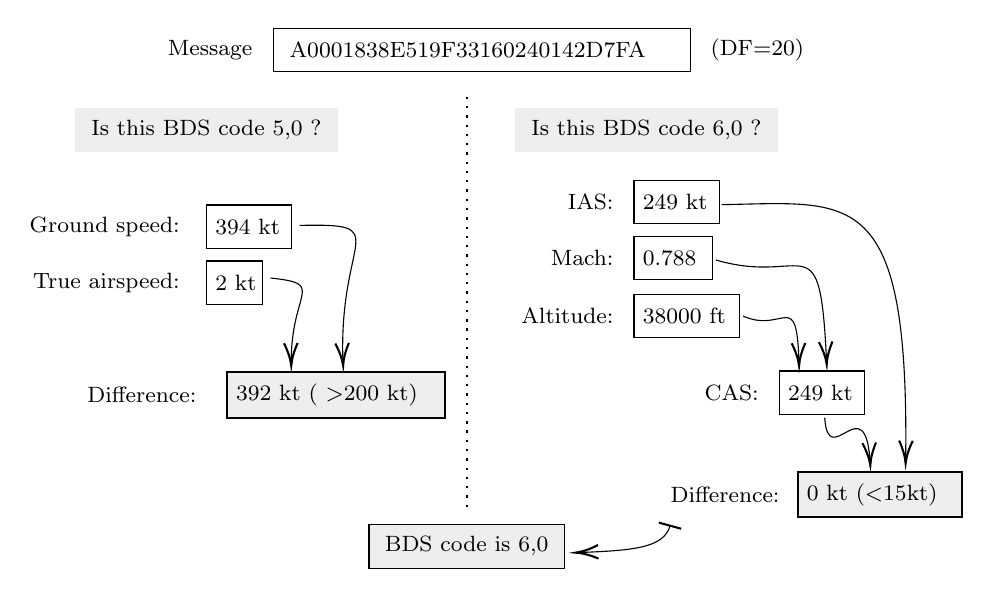
\begin{tikzpicture}[x=0.75pt,y=0.75pt,yscale=-1,xscale=1]
%uncomment if require: \path (0,348); %set diagram left start at 0, and has height of 348

%Curve Lines [id:da6430793918846669] 
\draw    (355.67,127) .. controls (399.45,139.94) and (405.61,106.34) .. (408.95,176.27) ;
\draw [shift={(409,177.33)}, rotate = 267.32] [color={rgb, 255:red, 0; green, 0; blue, 0 }  ][line width=0.75]    (10.93,-3.29) .. controls (6.95,-1.4) and (3.31,-0.3) .. (0,0) .. controls (3.31,0.3) and (6.95,1.4) .. (10.93,3.29)   ;
%Curve Lines [id:da32235700877254647] 
\draw    (368.67,154) .. controls (388.37,162.87) and (394.48,139.71) .. (395.62,176.29) ;
\draw [shift={(395.67,178)}, rotate = 268.53] [color={rgb, 255:red, 0; green, 0; blue, 0 }  ][line width=0.75]    (10.93,-3.29) .. controls (6.95,-1.4) and (3.31,-0.3) .. (0,0) .. controls (3.31,0.3) and (6.95,1.4) .. (10.93,3.29)   ;
%Curve Lines [id:da8301342497366322] 
\draw    (408,203) .. controls (409.97,229.6) and (427.46,187.3) .. (429.9,224.26) ;
\draw [shift={(430,226)}, rotate = 267.14] [color={rgb, 255:red, 0; green, 0; blue, 0 }  ][line width=0.75]    (10.93,-3.29) .. controls (6.95,-1.4) and (3.31,-0.3) .. (0,0) .. controls (3.31,0.3) and (6.95,1.4) .. (10.93,3.29)   ;
%Curve Lines [id:da14303571391445913] 
\draw    (358.33,100.33) .. controls (421.33,99.33) and (449,90) .. (447,225) ;
\draw [shift={(447,225)}, rotate = 270.85] [color={rgb, 255:red, 0; green, 0; blue, 0 }  ][line width=0.75]    (10.93,-3.29) .. controls (6.95,-1.4) and (3.31,-0.3) .. (0,0) .. controls (3.31,0.3) and (6.95,1.4) .. (10.93,3.29)   ;
%Curve Lines [id:da7746471843860618] 
\draw    (141,135.67) .. controls (168.25,138.62) and (150.87,141.25) .. (150.98,176.37) ;
\draw [shift={(151,178)}, rotate = 268.96] [color={rgb, 255:red, 0; green, 0; blue, 0 }  ][line width=0.75]    (10.93,-3.29) .. controls (6.95,-1.4) and (3.31,-0.3) .. (0,0) .. controls (3.31,0.3) and (6.95,1.4) .. (10.93,3.29)   ;
%Curve Lines [id:da5542954001907279] 
\draw    (155,110.33) .. controls (201.53,109.34) and (173.57,114.89) .. (175.92,176.13) ;
\draw [shift={(176,178)}, rotate = 267.27] [color={rgb, 255:red, 0; green, 0; blue, 0 }  ][line width=0.75]    (10.93,-3.29) .. controls (6.95,-1.4) and (3.31,-0.3) .. (0,0) .. controls (3.31,0.3) and (6.95,1.4) .. (10.93,3.29)   ;
%Straight Lines [id:da3827685237283216] 
\draw  [dash pattern={on 0.84pt off 2.51pt}]  (235.67,48.33) -- (235.67,249) ;
%Curve Lines [id:da8658759276112653] 
\draw    (333.5,255) .. controls (330.56,265.78) and (315.62,266.96) .. (289.61,267.94) ;
\draw [shift={(288,268)}, rotate = 357.88] [color={rgb, 255:red, 0; green, 0; blue, 0 }  ][line width=0.75]    (10.93,-3.29) .. controls (6.95,-1.4) and (3.31,-0.3) .. (0,0) .. controls (3.31,0.3) and (6.95,1.4) .. (10.93,3.29)   ;
\draw [shift={(333.5,255)}, rotate = 285.26] [color={rgb, 255:red, 0; green, 0; blue, 0 }  ][line width=0.75]    (0,5.59) -- (0,-5.59)   ;

% Text Node
\draw    (142.26,15.33) -- (343.26,15.33) -- (343.26,36.33) -- (142.26,36.33) -- cycle  ;
\draw (145.26,25.83) node [anchor=west] [inner sep=0.75pt]  [font=\footnotesize] [align=left] {\begin{minipage}[lt]{134.18644pt}\setlength\topsep{0pt}
\begin{center}
A0001838E519F33160240142D7FA
\end{center}

\end{minipage}};
% Text Node
\draw (133.51,25.83) node [anchor=east] [inner sep=0.75pt]  [font=\footnotesize] [align=left] {Message};
% Text Node
\draw    (110.12,100.5) -- (151.12,100.5) -- (151.12,121.5) -- (110.12,121.5) -- cycle  ;
\draw (113.12,111) node [anchor=west] [inner sep=0.75pt]  [font=\footnotesize] [align=left] {394 kt};
% Text Node
\draw (98.52,111) node [anchor=east] [inner sep=0.75pt]  [font=\footnotesize] [align=left] {Ground speed:};
% Text Node
\draw    (110.12,127.5) -- (137.12,127.5) -- (137.12,148.5) -- (110.12,148.5) -- cycle  ;
\draw (113.12,138) node [anchor=west] [inner sep=0.75pt]  [font=\footnotesize] [align=left] {2 kt};
% Text Node
\draw (98.52,138) node [anchor=east] [inner sep=0.75pt]  [font=\footnotesize] [align=left] {True airspeed:};
% Text Node
\draw    (316.12,88.5) -- (357.12,88.5) -- (357.12,109.5) -- (316.12,109.5) -- cycle  ;
\draw (319.12,99) node [anchor=west] [inner sep=0.75pt]  [font=\footnotesize] [align=left] {249 kt};
% Text Node
\draw (307.52,99) node [anchor=east] [inner sep=0.75pt]  [font=\footnotesize] [align=left] {IAS:};
% Text Node
\draw    (316.12,115.5) -- (354.12,115.5) -- (354.12,136.5) -- (316.12,136.5) -- cycle  ;
\draw (319.12,126) node [anchor=west] [inner sep=0.75pt]  [font=\footnotesize] [align=left] {0.788};
% Text Node
\draw (307.52,126) node [anchor=east] [inner sep=0.75pt]  [font=\footnotesize] [align=left] {Mach:};
% Text Node
\draw    (386.12,180.5) -- (427.12,180.5) -- (427.12,201.5) -- (386.12,201.5) -- cycle  ;
\draw (389.12,191) node [anchor=west] [inner sep=0.75pt]  [font=\footnotesize] [align=left] {249 kt};
% Text Node
\draw (377.52,191) node [anchor=east] [inner sep=0.75pt]  [font=\footnotesize] [align=left] {CAS:};
% Text Node
\draw    (316.12,143.5) -- (367.12,143.5) -- (367.12,164.5) -- (316.12,164.5) -- cycle  ;
\draw (319.12,154) node [anchor=west] [inner sep=0.75pt]  [font=\footnotesize] [align=left] {38000 ft};
% Text Node
\draw (307.52,154) node [anchor=east] [inner sep=0.75pt]  [font=\footnotesize] [align=left] {Altitude:};
% Text Node
\draw  [fill={rgb, 255:red, 238; green, 238; blue, 238 }  ,fill opacity=1 ][line width=0.75]   (120.12,181) -- (225.12,181) -- (225.12,203) -- (120.12,203) -- cycle  ;
\draw (123.12,192) node [anchor=west] [inner sep=0.75pt]  [font=\footnotesize] [align=left] {392 kt ( $\displaystyle  >$200 kt)};
% Text Node
\draw (106.52,192) node [anchor=east] [inner sep=0.75pt]  [font=\footnotesize] [align=left] {Difference:};
% Text Node
\draw  [fill={rgb, 255:red, 238; green, 238; blue, 238 }  ,fill opacity=1 ][line width=0.75]   (395.12,229) -- (474.12,229) -- (474.12,251) -- (395.12,251) -- cycle  ;
\draw (398.12,240) node [anchor=west] [inner sep=0.75pt]  [font=\footnotesize] [align=left] {0 kt ($\displaystyle < $15kt)};
% Text Node
\draw (387.52,240) node [anchor=east] [inner sep=0.75pt]  [font=\footnotesize] [align=left] {Difference:};
% Text Node
\draw  [draw opacity=0][fill={rgb, 255:red, 238; green, 238; blue, 238 }  ,fill opacity=1 ]  (46.65,53.83) -- (173.65,53.83) -- (173.65,74.83) -- (46.65,74.83) -- cycle  ;
\draw (110.15,64.33) node  [font=\footnotesize] [align=left] {Is this BDS code 5,0 ?};
% Text Node
\draw  [draw opacity=0][fill={rgb, 255:red, 238; green, 238; blue, 238 }  ,fill opacity=1 ]  (258.65,53.83) -- (385.65,53.83) -- (385.65,74.83) -- (258.65,74.83) -- cycle  ;
\draw (322.15,64.33) node  [font=\footnotesize] [align=left] {Is this BDS code 6,0 ?};
% Text Node
\draw  [color={rgb, 255:red, 0; green, 0; blue, 0 }  ,draw opacity=1 ][fill={rgb, 255:red, 238; green, 238; blue, 238 }  ,fill opacity=1 ]  (188.48,254.5) -- (282.48,254.5) -- (282.48,275.5) -- (188.48,275.5) -- cycle  ;
\draw (235.48,265) node  [font=\footnotesize] [align=left] {BDS code is 6,0};
% Text Node
\draw (351.8,25.83) node [anchor=west] [inner sep=0.75pt]  [font=\footnotesize] [align=left] {(DF=20)};


\end{tikzpicture}

\caption{Indenfication of BDS code, DF=20}
\label{fig:bds_bds_infer_example_1}
\end{figure}

We see that BDS 6,0 is identified since the difference between the ground speed and airspeed is too high in the BDS 5,0 assumption.

In Figure \ref{fig:bds_bds_infer_example_2}, the identification of a DF=21 message is shown. In DF=21 messages, the altitude code is not included. Thus, we have to reply to other information, such as speed and track angle from ADS-B to validate the BDS code. The assumption from BDS 5,0 conforms to the ADS-B information.

\begin{figure}[ht]
\centering



\tikzset{every picture/.style={line width=0.75pt}} %set default line width to 0.75pt        

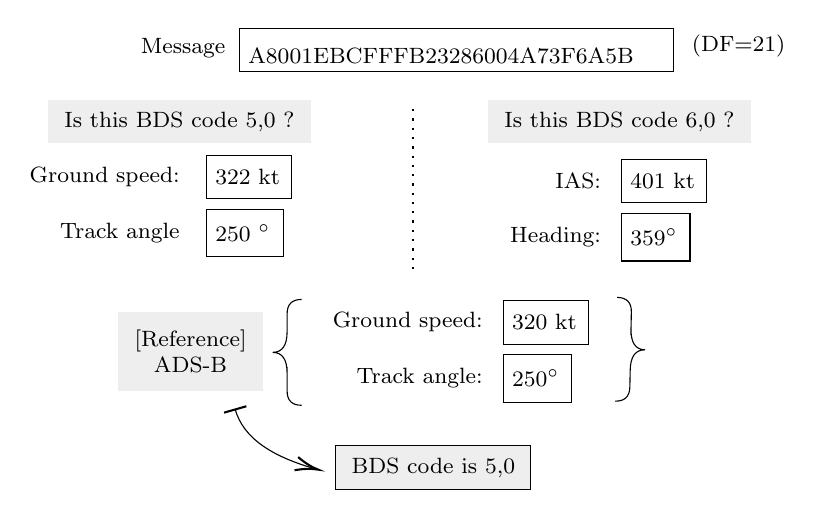
\begin{tikzpicture}[x=0.75pt,y=0.75pt,yscale=-1,xscale=1]
%uncomment if require: \path (0,348); %set diagram left start at 0, and has height of 348

%Straight Lines [id:da35241177696500303] 
\draw  [dash pattern={on 0.84pt off 2.51pt}]  (222.67,55.33) -- (222.67,133) ;
%Shape: Brace [id:dp1530573936144315] 
\draw   (169,147) .. controls (164.33,147) and (162,149.33) .. (162,154) -- (162,162.5) .. controls (162,169.17) and (159.67,172.5) .. (155,172.5) .. controls (159.67,172.5) and (162,175.83) .. (162,182.5)(162,179.5) -- (162,191) .. controls (162,195.67) and (164.33,198) .. (169,198) ;
%Shape: Brace [id:dp6255606362271318] 
\draw   (320,196) .. controls (324.67,196.09) and (327.05,193.81) .. (327.14,189.14) -- (327.3,181.14) .. controls (327.43,174.47) and (329.83,171.19) .. (334.5,171.28) .. controls (329.83,171.19) and (327.57,167.81) .. (327.7,161.14)(327.64,164.14) -- (327.86,153.14) .. controls (327.95,148.47) and (325.67,146.09) .. (321,146) ;
%Curve Lines [id:da4952815160936861] 
\draw    (137,200) .. controls (140.9,213.65) and (154.31,222.55) .. (175.37,228.54) ;
\draw [shift={(177,229)}, rotate = 195.26] [color={rgb, 255:red, 0; green, 0; blue, 0 }  ][line width=0.75]    (10.93,-3.29) .. controls (6.95,-1.4) and (3.31,-0.3) .. (0,0) .. controls (3.31,0.3) and (6.95,1.4) .. (10.93,3.29)   ;
\draw [shift={(137,200)}, rotate = 254.05] [color={rgb, 255:red, 0; green, 0; blue, 0 }  ][line width=0.75]    (0,5.59) -- (0,-5.59)   ;

% Text Node
\draw    (139.07,16.33) -- (348.07,16.33) -- (348.07,37.33) -- (139.07,37.33) -- cycle  ;
\draw (142.07,26.83) node [anchor=west] [inner sep=0.75pt]  [font=\footnotesize] [align=left] {\begin{minipage}[lt]{139.17356pt}\setlength\topsep{0pt}
\begin{center}
A8001EBCFFFB23286004A73F6A5B
\end{center}

\end{minipage}};
% Text Node
\draw (133.51,25.83) node [anchor=east] [inner sep=0.75pt]  [font=\footnotesize] [align=left] {Message};
% Text Node
\draw    (123.12,77.5) -- (164.12,77.5) -- (164.12,98.5) -- (123.12,98.5) -- cycle  ;
\draw (126.12,88) node [anchor=west] [inner sep=0.75pt]  [font=\footnotesize] [align=left] {322 kt};
% Text Node
\draw (111.52,88) node [anchor=east] [inner sep=0.75pt]  [font=\footnotesize] [align=left] {Ground speed:};
% Text Node
\draw    (123.12,103.5) -- (160.12,103.5) -- (160.12,126.5) -- (123.12,126.5) -- cycle  ;
\draw (126.12,115) node [anchor=west] [inner sep=0.75pt]  [font=\footnotesize] [align=left] {250 $\displaystyle ^{\circ }$};
% Text Node
\draw (111.52,115) node [anchor=east] [inner sep=0.75pt]  [font=\footnotesize] [align=left] {Track angle};
% Text Node
\draw    (323.12,79.5) -- (364.12,79.5) -- (364.12,100.5) -- (323.12,100.5) -- cycle  ;
\draw (326.12,90) node [anchor=west] [inner sep=0.75pt]  [font=\footnotesize] [align=left] {401 kt};
% Text Node
\draw (314.52,90) node [anchor=east] [inner sep=0.75pt]  [font=\footnotesize] [align=left] {IAS:};
% Text Node
\draw    (323.12,105.5) -- (356.12,105.5) -- (356.12,128.5) -- (323.12,128.5) -- cycle  ;
\draw (326.12,117) node [anchor=west] [inner sep=0.75pt]  [font=\footnotesize] [align=left] {359$\displaystyle ^{\circ }$};
% Text Node
\draw (314.52,117) node [anchor=east] [inner sep=0.75pt]  [font=\footnotesize] [align=left] {Heading:};
% Text Node
\draw  [draw opacity=0][fill={rgb, 255:red, 238; green, 238; blue, 238 }  ,fill opacity=1 ]  (46.65,50.83) -- (173.65,50.83) -- (173.65,71.83) -- (46.65,71.83) -- cycle  ;
\draw (110.15,61.33) node  [font=\footnotesize] [align=left] {Is this BDS code 5,0 ?};
% Text Node
\draw  [draw opacity=0][fill={rgb, 255:red, 238; green, 238; blue, 238 }  ,fill opacity=1 ]  (258.65,50.83) -- (385.65,50.83) -- (385.65,71.83) -- (258.65,71.83) -- cycle  ;
\draw (322.15,61.33) node  [font=\footnotesize] [align=left] {Is this BDS code 6,0 ?};
% Text Node
\draw  [color={rgb, 255:red, 0; green, 0; blue, 0 }  ,draw opacity=1 ][fill={rgb, 255:red, 238; green, 238; blue, 238 }  ,fill opacity=1 ]  (185.48,217.5) -- (279.48,217.5) -- (279.48,238.5) -- (185.48,238.5) -- cycle  ;
\draw (232.48,228) node  [font=\footnotesize] [align=left] {BDS code is 5,0};
% Text Node
\draw (355.8,24.83) node [anchor=west] [inner sep=0.75pt]  [font=\footnotesize] [align=left] {(DF=21)};
% Text Node
\draw    (266.12,147.5) -- (307.12,147.5) -- (307.12,168.5) -- (266.12,168.5) -- cycle  ;
\draw (269.12,158) node [anchor=west] [inner sep=0.75pt]  [font=\footnotesize] [align=left] {320 kt};
% Text Node
\draw (257.52,158) node [anchor=east] [inner sep=0.75pt]  [font=\footnotesize] [align=left] {Ground speed:};
% Text Node
\draw    (266.12,173.5) -- (299.12,173.5) -- (299.12,196.5) -- (266.12,196.5) -- cycle  ;
\draw (269.12,185) node [anchor=west] [inner sep=0.75pt]  [font=\footnotesize] [align=left] {250$\displaystyle ^{\circ }$};
% Text Node
\draw (257.52,185) node [anchor=east] [inner sep=0.75pt]  [font=\footnotesize] [align=left] {Track angle:};
% Text Node
\draw  [draw opacity=0][fill={rgb, 255:red, 238; green, 238; blue, 238 }  ,fill opacity=1 ]  (80.48,153) -- (150.48,153) -- (150.48,191) -- (80.48,191) -- cycle  ;
\draw (115.48,172) node  [font=\footnotesize] [align=left] {\begin{minipage}[lt]{44.88pt}\setlength\topsep{0pt}
\begin{center}
[Reference]\\ADS-B
\end{center}

\end{minipage}};


\end{tikzpicture}

\caption{Indenfication of BDS code, DF=21}
\label{fig:bds_bds_infer_example_2}
\end{figure}

\begin{notebox}{Try it out}
Using \texttt{pyModeS}, we can infer the BDS code of a message as: 

\begin{verbatim}
import pyModeS as pms

msg1 = "A0001838E519F33160240142D7FA"
bds1 = pms.bds.infer(msg1)

msg2 = "A8001EBCFFFB23286004A73F6A5B"
bds2 = pms.bds.infer(msg2)
\end{verbatim}

This first BDS code should be \texttt{BDS60} and the secodn one should be \texttt{BDS50}.

\end{notebox}


\part{Conclusions}
% \chapter{The use of Mode S data}
% \section{Trajectory construction}
% \section{Application of surveillance data}
% \section{Congestion}
% \section{Crowd-sourced networks}
% \section{Conclusion}

\chapter{Conclusion}

Finally, we have come to the end of this book. We started with the fundamental 


\chapter*{References}
\addcontentsline{toc}{chapter}{References}
\printbibliography[heading=none]

\chapter*{Acknowledgements}

{
\setstretch{1.0}
I could not have completed this book without the support of my wife, Marie. She proofread every word in this book and gave valuable inputs on its content. I want to thank my parents for their encouragement of my curiosity and scientific endeavors since childhood. My sons, William and Vincent, make my life and research more joyful; for example, I always feel happy to see they are curious and enthusiastic to see me testing antennas, receivers, and hardware.

Navigating through the mountain of information in different ICAO documents is complicated. I am grateful to have met Huy V\^u and supervised his master thesis project. He was able to find almost any needed information regarding Mode~S, which was a great help for this book and the pyModeS library. He is now a data analyst at \emph{LVNL}, the Dutch air traffic control, and we still work together on interesting research topics. 

In the summer of 2017, I received an email from a researcher from \emph{ONERA}, the French aerospace research institute, who wanted to meet me for a coffee to discuss Mode S. That coffee discussion with Xavier Olive has turned into a fruitful collaboration. I want to say thanks to Xavier for his inputs on Mode S, ADS-B, and all other related and unrelated discussions.

Before even the notion of this book existed, I was a new PhD student at the CNS/ATM research group. I would like to thank Jacco Hoekstra and Joost Ellerbroek, who were my promotors and provided me with great support for all my PhD research topics. I am also extremely grateful to be able to continue working with them as a colleague since 2019. I would also like to extend my thanks to the Dean of our faculty, Henri Werij, for his consistent support and for offering me the opportunity to continue my research at the faculty. 

My research often relies on Mode S and ADS-B data from regions beyond the coverage of our antenna in Delft. This is only possible with the help of crowd-sourced networks. I want to thank Martin Strohmeier from \emph{OpenSky network}, Sean Atkinson from \emph{FlightRadar24}, and James Stanford from \emph{ADS-B Exchange} for sharing their data with me for different research projects over the past years.

The manual was an open-access book from the beginning. I heartily appreciate all the GitHub contributors who made suggestions and edits for this book and pyModeS library.\footnote{The most up-to-date list of contributors can be found at: \\https://github.com/junzis/the-1090mhz-riddle/graphs/contributors \\https://github.com/junzis/pyModeS/graphs/contributors} Since I decided to publish this book with TU Delft OPEN Publishing, our publishing officer, Frederique Belliard, has been extremely helpful in making this book a reality. Finally, I would also like to thank Petr Jonas, Xavier Olive, Enrico Spinielli, and Huy V\^u for their comprehensive peer-review that led to the successful completion of this book.
}
\chapter*{About the Author}

Junzi Sun is an assistant professor at TU Delft, currently working in the CNS/ATM chair, Control and Simulation group, at the Aerospace Engineering Faculty. He is passionate about open-source, open science, and making air transportation more sustainable.

He was born in China and completed his bachelor’s degree in telecommunication at Beijing University of Posts and Telecommunications. Then, He moved to Europe and obtained his master’s degree in aerospace at Polytechnic University of Catalonia. After that, he worked in Spain and France for a few years before continuing his doctoral research in the Netherlands, where he obtained his Ph.D. degree and currently work and live.


% \clearpage
% \addcontentsline{toc}{chapter}{Index}
% \printindex

\end{document}
